\documentclass{article}

\author{Alexandry Augustin}
\title{A Parametric Approach To Bayesian Drift Estimation of Discretely Observed Price Diffusion Processes}

%\usepackage{breqn}

%\begin{equation}\label{t:est}
%\end{equation}
%\ref{t:est}
%\eqref{t:est}

%\usepackage{subeqn}

\usepackage{mathrsfs}
\usepackage{amsmath} % align*
\usepackage{graphicx}
\graphicspath{{./res/}}
\usepackage{amssymb} % \therefore
\usepackage[justification=centering]{caption} %line break in figures captions

\usepackage{listings} %for source code
\lstset{numbers=left, stepnumber=1, language=Matlab, basicstyle=\footnotesize, numberstyle=\footnotesize} %frame=single

\usepackage{nonfloat}
%-------
% Layout
%-------
%\addtolength{\oddsidemargin}{-.875in}
%\addtolength{\evensidemargin}{-.875in}
%\addtolength{\textwidth}{1.75in}

%\addtolength{\topmargin}{-.875in}
%\addtolength{\textheight}{1.75in}

%----------------
% Thm environment
%----------------
\usepackage{amsthm} %Theorems

\newtheorem{axiom}{Axiom}
\newtheorem{thm}{Theorem}[section]
\newtheorem{prop}[thm]{Proposition}
\newtheorem{lem}[thm]{Lemma}
\newtheorem{cor}[thm]{Corollary}

\theoremstyle{definition}
\newtheorem{definition}[thm]{Definition}
\newtheorem{example}[thm]{Example}

\theoremstyle{remark}

\newtheorem{remark}[thm]{Remark}

%-----------
% newcommand
%-----------
\newcommand{\filtration}[1]{\ensuremath{\mathscr{F}_{#1}}}
\newcommand{\filtrationObs}[1]{\ensuremath{\mathscr{Y}_{#1}}}
\newcommand{\market}{\ensuremath{\mathscr{M}}}
\newcommand{\measure}[1]{\ensuremath{\mathbb{#1}}}
\newcommand{\m}[1]{\ensuremath{\mathbf{#1}}}
\newcommand{\Ito}{It\^{o} }

\newcommand{\ep}[1]{\ensuremath{E^{\mathbb{P}}[#1]}}
\newcommand{\eq}[1]{\ensuremath{E^{\mathbb{Q}}[#1]}}
\newcommand{\girsanov}[3]{\ensuremath{
	\measure{#1}(E)=\int_E e^{#2} d\measure{#3}
	}}
\newcommand{\girsanovBis}[3]{\ensuremath{
	\measure{#1}^i(E)=\int_E {#2} d\measure{#3}
	}}
\newcommand{\strategy}{\ensuremath{(\phi, \psi)}}
\newcommand{\gain}{\ensuremath{\int_0^t \phi_sdS_s+\int_0^t\psi_sdB_s}}
\newcommand{\I}[1]{\ensuremath{I_{\{#1\}}}}
\newcommand{\stdnormal}{\ensuremath{\frac{1}{\sqrt{2\pi}}e^{-\frac{1}{2}x^2}}}
\newcommand{\stdcumnormal}[1]{\ensuremath{\frac{1}{\sqrt{2\pi}}\int_{-\infty}^{#1}e^{-\frac{1}{2}u^2}du}}
\newcommand{\cumnormal}{\ensuremath{\frac{1}{\sqrt{2\pi}\sigma}\int_{-\infty}^xe^{-\frac{1}{2}\left( \frac{u-\mu}{\sigma}\right)^2}du}}
\newcommand{\normal}{\ensuremath{\frac{1}{\sigma\sqrt{2\pi}}e^{-\frac{1}{2}\left(\frac{x-\mu}{\sigma}\right)^2}}}
\newcommand{\CumNormalGeneric}[3]{\ensuremath{\frac{1}{\sqrt{2\pi}#3}\int_{-\infty}^{#1}e^{-\frac{1}{2}\left( \frac{u-#2}{#3}\right)^2}du}}
\newcommand{\CumNormalGenericNoMu}[3]{\ensuremath{\frac{1}{\sqrt{2\pi}#2}\int_{-\infty}^{#1}e^{-\frac{1}{2}\left( \frac{#3}{#2}\right)^2}du}}

\newcommand{\call}[1]{\ensuremath{C_#1(#1, S_#1)}}
\newcommand{\discall}[1]{\ensuremath{\tilde{C_#1}(#1, S_#1)}}

\newcommand{\done}{\ensuremath{\frac{ln\left( \frac{F_t}{K}\right)+\frac{\sigma^2}{2}(T-t)}{\sigma\sqrt{T-t}}}}
\newcommand{\donebis}{\ensuremath{\frac{ln\left( \frac{S_0}{K}\right)+\left( r-q+\frac{\sigma^2}{2}\right)T}{\sigma\sqrt{T}}}}
\newcommand{\dtwo}{\ensuremath{\frac{ln\left( \frac{S_0}{K}\right)+\left( r-q-\frac{\sigma^2}{2}\right)T}{\sigma\sqrt{T}}}}

\newcommand{\process}[1]{\ensuremath{(#1_t)_{t>0}}}
\newcommand{\processD}[1]{\ensuremath{(#1_k)_{k>0}}}

\begin{document}

\begin{center}
\begin{center}
%Parametric Recursive Bayesian Estimation for the Drift from Discretely Observed Diffusion Price Processes
{\large \bfseries A Parametric Approach To Bayesian Drift Estimation of Discretely Observed Price Diffusion Processes\footnote{I would like to cordially thank Dr. Chris Barnett for his advice and help in the production of this work.}}
\end{center}
\bigskip
Alexandry AUGUSTIN \\
\bigskip
September 19, 2011\\
\bigskip\bigskip
Department of Mathematics\\
Imperial College of Science, Technology and Medicine\\
London SW7 2BZ\\

%\smallskip
\bigskip\bigskip\bigskip
Project report submitted in partial fulfilment of the degree of MSc in
Mathematics and Finance at Imperial College London.
\bigskip\bigskip\bigskip

%Summer project
\end{center}
\begin{abstract}
%\section*{Abstract}
The present report suggests an approach to parametric estimation of the drift function $\mu(t)$ in a one-dimensional \Ito stochastic differential equation representing a stock price with a variable diffusion parameter $\sigma$ such that $dS_t=\mu(t)S_tdt+\sigma S_tdW_t$ from a portfolio consisting of the stock, a call option and a forward contract. The parametric charactrisation of $\mu(t)$ will be derived from non-arbitrage arguments used to price derivatives  - Black-Scholes (1970). The stock price process will be expressed in terms of discretely observed derivative prices and the unobservable discrete \emph{market risk premium}, the later modeled using the Ornstein--Uhlenbeck process. To address the time variation of volatility $\sigma$, the \emph{Black-Scholes implied volatility} of the option will be used. The resulting system of prices and market risk premium dynamics will then be cast into the \emph{state space} framework from which the time varying conditional distribution of the market risk premium can be estimated using the \emph{Kalman filter} - Kalman (1960). Numerical analysis will be carried out using simulated market prices.
\\
\\
%We will show that we can estimate the dynamic drift $\mu(t)=r-q+\sigma \lambda(t)$ of the stock index price for a portfolio consisting of the stocks, a call option and a forward contract under the real market measure \measure{P} in the no-arbitrage framework through the market price of risk $\lambda(t)$. 
\textit{Keywords}: \Ito Diffusion, Market price of risk, Risk-neutral valuation, Euler-Maruyama scheme, Linear recursive Baysian estimation, Kalman filter, Stochastic filtering.
\end{abstract}



\newpage
\tableofcontents
\setcounter{tocdepth}{10}
% add abstract+appendix

%\newpage
%\section*{Notations}
%$N(x)=\stdcumnormal{x}$          Standard cumulative normal distribution\\
%$\measure{P}$\\
%$\measure{Q}$\\
%\filtration{t}\\
%$E^\measure{Q}_t[.]=E^\measure{Q}[.|\filtration{t}]$\\

\newpage
\section{Introduction}

%On the other hand, it is an arbitrage-free and complete model. 
%Th�orie de la sp�culation

The recovery of information from measurements corrupted by uncertainty has long been a struggle endured by many investors. Typical to financial asset prices, the volatility is usually very large compare to the drift resulting in difficult accurate estimation. \\
\\
\emph{Stochastic processes} are a natural choice to model the time evolution of financial assets subject to random influences. Historically, Louis Bachelier is credited with being the first to model stock prices with stochastic processes (using a Brownian motion), which was part of his PhD thesis \emph{The Theory of Speculation} (1900). However, price in his model could assume negative values and therefore couldn't reflect the reality of the market. Subsequently, Black-Scholes developed in \emph{The Pricing of Options and Corporate Liabilities} (1973) where the stock price follows a geometric brownian motion with drift (see appendix A). While derivative valuation models presuppose knowledge of the parameters that underlie diffusion processes, in practice these parameters are unknown and must be estimated (commonly referred as \emph{model calibration}).\\
\\%\emph{signal} or \emph{information}
The development of \emph{stochastic filtering} theory in the early 1940s pioneered by Wiener (1942) and Kolmogorov (1941) provides us with the necessary tools to make reasonable inferences about the unknown diffusion parameters. In particular, \emph{Bayesian filtering} is aimed to apply Bayes statistics to stochastic filtering problems. It culminated with the publication of \emph{A new approach to linear fitering and prediction problem} by Kalman (1960) where the classic \emph{Kalman filter} was introduced \footnote{Bucy (1961) derived the continuous time counterpart independently in what is now called the \emph{Kalman-Bucy filter}.}.\\
\\% and appendix ? for an example from classical mechanics
The first full implementation of the Kalman filter was in 1960 at the \emph{Ames Research Center} (NASA) where it was used for the trajectory estimation and control problem of the Apollo project. In particular, the Apollo 11 lunar module that landed to the moon was guided by a Kalman filter. The filter performed inference on the module position based on multiple embeded sensors which was then compared to earth-based estimates. If they had disagreed too much the mission would have had to be aborted - see Mohinder and Angus (2001) for historical accounts and appendix \ref{sec:meca} for an example from classical mecanics. Nowadays, Kalman filters have been applied in various scientific areas, including communications, machine learning, finance, economics, etc. It has been said that the Kalman filter is the greater discoveries in the history of statistical estimation theory.\\
\\
The point of view taken here is that scientific inferences made about financial phenomena are not fundamentally different from inference made about phenomena in other areas of science (namely \emph{engineering}). Thinking aside leads to a richer variety of ideas from which combinations can be formed.\\
\\
\textit{"The unity of all science consists alone in its method, not in its material."} - Karl Pearson (1892), The Grammar of Science.
\\

%"Indeed, it is ovious that invention or discovery, be it in mathematics or anywhere else, takes place by combining ideas."- Jacques Hadamard, The Psychology of Invention in the Mathematical Field,  1945.
%These combinations are formed in both the conscious and unconscious minds and it is the task of the researcher to avoid choosing useless combinations and to select only thos that are useful. Thinking aside leads to a richer variety of ideas from which combinations can be formed. "Sudden inspirations never happen except after some days of voluntary effort which has appeared absolutely fruitless and whence nothing good seems to have come, where the way taken seems totally astray.". The preparatory work period is accompanied and followd by an incubation period and finally by illumination. 
%"An Introduction to Bayesian Inference in Econometrics", Zellner

%The development of the linear filtering theory using the state space approach was carried out by Kalman.

Although many methods currently exist to estimate diffusion processes, the method proposed in this report is applicable to a large class of discretly observed diffusion processes, including those for which observations are irregularly spaced, those in which the data are observed with error due to factors such as market microstructure. \\
\\
% and frequent recapitulations were added
The report is organized as follows. Chapter 1 provide the fundation for the parametric system based on the risk-neutral valuation framework. Chapter 2 is a self contained derivation of the Kalman filtering equations from a Bayesian filtering standpoint. Chapter 3 addresses the estimation problem of the diffusion parameter $\mu_k$ identified in Chapter 1. In each Chapters particular areas have been addressed where the views clearly advanced the general objective. Otherwise, detailed proofs and further more-detailes have been relegated to the appendix section so as not to interupt the flow of reading.
%The select bibliography is very select. 
The select bibliography is intended mainly to give references to specific secondary literature cited in the text, although other influential works have been included as well. 

%We will not consider the problem of data and will take the data as given.







\newpage
\section{Market Price of Risk in the Risk-Neutral Valuation Framework}\label{sec:riskn}
In this section will be described the risk-neutral relationship between the prices of the traded derivatives and their underlying assets.

%\begin{definition}
\begin{tabbing}\\
Let \= $(\Omega, \filtration{t}, P)$ be a complete filtered probability space where the filtration \\$\filtration{t}$  satisfies the \emph{usual conditions}:\\
\>(i) non-decreasing: $\filtration{s} \subseteq \filtration{t} \subset \filtration{}$ for $s \leq t$,\\
\>(ii) right continuity: $\filtration{t}=\filtration{t^{+}}=\cap_{u>t} \filtration{u}$,\\
\>(iii) completness: \filtration{0} contains all P-null sets of \filtration{}.
\end{tabbing}
Such a complete filtered probability space satisfying the usual conditions is called a \emph{stochastic basis}.\\
%\end{definition}
\\
On this stochastic basis, the filtration $\filtration{t}$ is the sigma-field generated by a standard one-dimensional Brownian motion \process{W} such that 
\begin{equation*}
\filtration{t}=\sigma\{W_t\}.
\end{equation*}

We model the stock index price as a one-dimensional time-inhomogeneous \Ito diffusion process 
%\begin{equation}
%S_t=S_0e^{\int_0^t(\mu(t)-\frac{\sigma^2}{2})ds+\sigma dW_t}
%\end{equation}
\begin{equation}\label{eq:stockDyn}
%dS_t=\mu(S_t, t)dt+\sigma(S_t, t)dW_t
dS_t=\mu(t)S_tdt+\sigma S_tdW_t.
\end{equation}
We denote $\mu(t)$ the unknown time--dependent \textit{drift function} and $\sigma^2$ the \emph{variance}.  \\
\\
We recall that the dynamic of a riskless bond is given by 
\begin{equation}\label{eq:bondDyn}
dB_t=B_tr(t)dt.
\end{equation}
We assume the existance of a \emph{forward contract} on \process{S} such that
\begin{equation}
dF_t=\mu_f(t) F_tdt + \sigma_f F_tdW_t. 
\end{equation}

Suppose that there is a \emph{call option} on \process{F} and its price process is \process{C}. We assume \process{F} is adapted to the filtration \filtration{t}, and in particular that \process{C} is fully characterised by an \filtration{T}-measurable terminal value $C_T=(F_t-K)^+$. We can write under $P$, 
\begin{equation}
dC_t = \mu_c(t)C_t dt + \sigma_c C_t dW_t
\end{equation}
for the price dynamics of the option. \\
\\
In summary, we are left with the following price dynamics to estimate $\mu(t)$
\begin{equation}\label{eq:sys1}
\boxed{
\left\{ \begin{array}{lcrcr}
          dS_t & = & \mu(t)S_t dt & + & \sigma S_t dW_t \\ 
          dF_t & = & \mu_f(t) F_tdt & + & \sigma_f F_tdW_t \\ 
          dC_t & = & \mu_c(t)C_tdt & + & \sigma_c C_tdW_t.
        \end{array} \right. 
}
\end{equation}
\\
Before proceeding further, we give the following definitions.





\subsection{Preliminary Definitions}
\begin{definition}
A \textit{portfolio process} \process{V} in the market $\market =(S_t, F_t, C_t, B_t)$ is a stochastic linear combination of $S_t$, $F_t$, $C_t$, $B_t$ such that
\begin{equation}
V_t=\phi_tS_t+\varphi_t F_t + \psi_t C_t + \xi_t B_t
\end{equation}
where $\phi_t$, $\varphi_t$, $\psi_t$, $\xi_t$ are progressively measurable adapted processes indicating the number of respective assets held at time $t$. We suppose that the assets are infinitely divisible and can be borrowed ("shorted") so that it is possible to hold any positive or negative quantities of either assets.
\end{definition}

\begin{definition}
The portfolio process \process{V} is \textit{self-financing} if
\begin{align}
dV_t=\phi_t dS_t+\varphi_t dF_t + \psi_t dC_t+q\phi_tS_tdt+\xi_t dB_t.
\end{align}
\end{definition}
That is, eventual incomes (selling assets, receiving dividends, ...) are exactly offset by required payments (buying additional assets, transaction costs, ...). And therefore the change in the portfolio value is only due to the trading profits and losses.\\
\\
The no-arbitrage argument is crucial for the existence of a risk-neutral measure. In fact, the condition of no-arbitrage is equivalent to the existence of a risk-neutral measure\footnote{See \emph{fundamental theorem of asset pricing}.}.
\begin{definition}
An \textit{arbitrage opportunity} is a self-financing portfolio \process{V} with the property that
$$V_0 = 0,$$
$$P(V_T \geq 0)=1,$$
$$P(V_T >0)>0.$$
\end{definition}
In other word, starting with no initial capital a $t=0$, the portfolio process \process{V} has a positive probability of gaining value at time $t=T$ with no exposure to risk.\\
\\
To avoid arbitrage opportunities, possible strategies need to be restricted to a subset whose wealth is bounded uniformly from below by a constant\footnote{See Biagini and Cerny (2011) for a complete presentation.}.
%an admissible strategy is defined as a predictable self-financing process that yields non-negative wealth at any time.
\begin{definition}
A strategy $(\phi_t,\varphi,\psi,\xi)$ is \textit{admissible} if for an integrable, non-negative and \filtration{T}-measurable random variable $X$, 
\begin{equation}
\frac{V_t}{B_t} \geq -E^P[X|\filtration{t}].
\end{equation}
\end{definition}

%\begin{definition}
%complete market
%\end{definition}






%Suppose that all the dividends are immediately reinvested in the stock, so that there is no cash position in the portfolio at any time.

\subsection{The Risk-Neutral Framework}
In this section we will derive an expression for all the parameters of the diffusion processes \eqref{eq:sys1} under the risk-neutral assumption.

\begin{prop}\label{prop:riskn1}
The conditions for the portfolio consisting of the stock index $S_t$ paying dividends at a constant rate $q$, the forward on the stock index $F_t$ and the call option on the forward $C_t$ to be risk-neutral are given by

%\begin{equation}
%\left\{ \begin{array}{lcl}
%          \mu(t) & = & (r-q)+\lambda(t) \sigma \\ 
%          \mu_f(t) & = & \lambda(t) \sigma_f \\ 
%          \mu_c(t) & = & r+\lambda(t) \sigma_c
%        \end{array} \right. 
%\end{equation}

\begin{subequations}
\begin{equation}
\mu(t) = (r-q)+\lambda(t) \sigma \label{eq:mu}
\end{equation}
\begin{equation}
\mu_f(t) = \lambda(t) \sigma_f
\end{equation}
\begin{equation}
\mu_c(t) = r+\lambda(t) \sigma_c
\end{equation}
\end{subequations}
where $\lambda(t)$ is known as the time-dependent \emph{markert price of risk}.
\end{prop}

\begin{proof}
Let the portfolio $V_t=\phi_tS_t+\varphi_t F_t + \psi_t C_t + \xi_t B_t$ consisting of a stock $S_t$ and a forward option on the stock $F_t$, a call option on the forward $C_t$ and a riskless bond $B_t$.\\
\\
It should be stressed at this point that dividend paying underlyings have divergent treatments in the literature. We will asume here that the accumulated value of the dividend stream $q\phi_tS_tdt$ is reinvested into the bond as to ensure that the portfolio is self-financing. We can write its dynamic as
\begin{align*}
dV_t=\phi_t dS_t+\varphi_t dF_t + \psi_t dC_t+q\phi_tS_tdt+\xi_t dB_t.
%&=()-\phi_t()
\end{align*}
Substituting \eqref{eq:sys1} from this expression, we get
\begin{align*}
dV_t=&\left[ \phi_t\mu(t)S_t+\varphi_t\mu_f(t)F_t+\psi_t\mu_c(t)C_t+q\phi_t S_t+\xi_tr(t)B_t \right]dt\\
&-\left[ \phi_t \sigma S_t+\varphi_t\sigma_f F_t+\psi_t\sigma_c C_t \right]dW_t.
\end{align*}
The portfolio is rendered riskless if 
\begin{equation}\label{eq:condone}
\left[ \phi_t \sigma S_t+\varphi_t\sigma_f F_t+\psi_t\sigma_c C_t \right]=0.
\end{equation}
The riskless dynamic of $V_t$ is then given by
\begin{align*}
\frac{dV_t}{V_t}&=\left(\frac{\phi_t\mu(t)S_t+\varphi_t\mu_f(t)F_t+\psi_t\mu_c(t)C_t+q\phi_t S_t+\xi_tr B_t}{\phi_tS_t+\varphi_t F_t + \psi_t C_t + \xi_t B_t}\right)dt.
\end{align*}
A riskless portfolio must earn the risk-free rate $r$, therefore
\begin{equation}\label{eq:condtwo}
\frac{\phi_t\mu(t)S_t+\varphi_t\mu_f(t)F_t+\psi_t\mu_c(t)C_t+q\phi_t S_t+\xi_tr(t)B_t}{\phi_tS_t+\varphi_t F_t + \psi_t C_t + \xi_t B_t}=r
\end{equation}
giving
\begin{align*}
(\mu(t)+q-r)\phi_tS_t+(\mu_f(t)-r)\varphi_t F_t+(\mu_c(t)-r)\psi_t C_t=0.
\end{align*}
Defining
\begin{equation*}
\left\{ \begin{array}{rc}
			X&=\phi_tS_t\neq 0\\
			Y&=\varphi_t F_t\neq 0\\
			Z&=\psi_t C_t\neq 0
        \end{array} \right. 
\end{equation*}
we can write the conditions \eqref{eq:condone} and \eqref{eq:condtwo} as
\begin{subequations}
\begin{align}
\sigma X &+& \sigma_f Y &+& \sigma_c Z & = 0 \label{eq:cond_one}\\ 
(\mu(t)+q-r)X &+& (\mu_f(t)-rY &+& (\mu_c(t)-r)Z & = 0.\label{eq:cond_two}
\end{align}
\end{subequations}
%\begin{equation}
%\left\{ \begin{array}{rcrcrc}
%          \sigma(t)X &+& \sigma_f(t)Y &+& \sigma_c(t)Z & = 0 \\ 
%          (\mu(t)+q-r(t))X &+& (\mu_f(t)-r(t))Y &+& (\mu_c(t)-r(t))Z & = 0.
%        \end{array} \right. 
%\end{equation}
Eliminating $X$ by subtracting $\sigma\times \eqref{eq:cond_two}$ from $(\mu(t)+q-r)\times \eqref{eq:cond_one}$ we get
\begin{align*}
&\left[ \sigma_f(\mu(t)+q-r)-\sigma(\mu_f(t)-r) \right]Y\\
+&\left[ \sigma_c(\mu(t)+q-r)-\sigma(\mu_c(t)-r) \right]Z=0.
\end{align*}
From the first term we get
\begin{equation*}
\frac{\mu(t)+q-r}{\sigma}=\frac{\mu_f(t)-r}{\sigma_f}
\end{equation*}
and from the second term we get
\begin{equation*}
\frac{\mu(t)+q-r}{\sigma}=\frac{\mu_c(t)-r}{\sigma_c}.
\end{equation*}
Therefore
\begin{equation*}
\frac{\mu(t)+q-r}{\sigma}=\frac{\mu_f(t)-r}{\sigma_f}=\frac{\mu_c(t)-r}{\sigma_c}=\lambda(t).
\end{equation*}
%giving
%\begin{equation}
%\left\{ \begin{array}{lcl}
%          \mu(t) & = & (r-q)+\lambda(t) \sigma \\ 
%          \mu_f(t) & = & \lambda(t) \sigma_f \\ 
%          \mu_c(t) & = & r+\lambda(t) \sigma_c
%        \end{array} \right. 
%\end{equation}
%which complete the proof.
We observe here that our result differs from the one obtained by Bhar, Chiarella and Runggaldier (2001) i.e.
\begin{equation*}
\frac{\mu(t)+q-r}{\sigma}=\frac{(\mu_f(t)+r)-r}{\sigma_f}=\frac{\mu_c(t)-r}{\sigma_c}=\lambda(t).
\end{equation*}
It seems that the traitement of dividends in the modeling of the assets is the source of the discrepancy. Further investigations needs to be done in order to complete accurately the proof (the approach taken by Musiela and Rutkowski in \emph{Martingale methods in financial modelling} seems to be of particular interest).\\
\\
Furthermore, the bond included in our portfolio (where the dividends are being re-invested) doesn't seems to be present in Bhar, Chiarella and Runggaldier (2001) derivations. We might question the importance of its inclusion in our portfolio.
\end{proof}




\begin{prop}\label{prop:riskn2}
The volatility of the Forward $\sigma_f$ is the same as it's underlying (the stock index price) $\sigma$,
\begin{equation}
	\boxed{\sigma_f = \sigma}
\end{equation}
\end{prop}
\begin{proof}
The discounted conditional expectation of the forward payoff under the risk-neutral measure is given by
\begin{align*}
f_t&=E^\measure{Q}_t[(S_T-K)e^{-r(T-t)}]\\
&=e^{-r(T-t)}(E^\measure{Q}_t[S_T]-K).
\end{align*}
The forward price process $F_t$ is the value of $K$ such that $f_t=0$. Therefore,
\begin{align*}
F_t&=E^\measure{Q}_t[S_T]\\
&=E^\measure{Q}_t[S_te^{(r-q-\frac{\sigma^2}{2})(T-t)+\sigma(W_T^\measure{Q}-W_t^\measure{Q})}]\\
&=S_te^{(r-q-\frac{\sigma^2}{2})(T-t)}E^\measure{Q}_t[e^{\sigma(W_T^\measure{Q}-W_t^\measure{Q})}].\\
\end{align*}
Identifying the expectation as the moment generating function\footnote{We recall that the moment generating function of a normally distributed random variable $X\sim N(\mu, \sigma)$ is given by $E[e^{tX}]=e^{t\mu+\frac{1}{2}t^2\sigma^2}$.} of $W_T^\measure{Q}-W_t^\measure{Q}\sim N(0, T-t)$ we get 
\begin{align}
F_t&=S_te^{(r-q-\frac{\sigma^2}{2})(T-t)}e^{\frac{\sigma^2}{2}(T-t)}\notag\\
&=S_te^{(r-q)(T-t)}.\label{eq:fwd}
\end{align}


%====================
%No arbitrage spot/futures price relationship is,
%where r is the risk-free rqte of interest, q the continous divident yield on the index qnd T is the mqturity dqte of the index futures. 
Applying the \emph{\Ito's product rule} gives 
\begin{align*}
dF_t &= S_tde^{(r-q)(T-t)}+e^{(r-q)(T-t)}dS_t+\left<S_t,e^{(r-q)(T-t)}\right>\\
\end{align*}
with 
\begin{equation*}
\frac{de^{(r-q)(T-t)}}{dt}=-(r-q)e^{(r-q)(T-t)}
\end{equation*}
and 
\begin{equation*}
\left<S_t,e^{(r-q)(T-t)}\right>=0
\end{equation*}
as $e^{(r-q)(T-t)}$ is a continuous finite variation processes. Therefore
\begin{align*}
dF_t &= -(r-q)S_te^{(r-q)(T-t)}dt+e^{(r-q)(T-t)}(\mu(t)S_tdt+\sigma S_tdW_t)\\
\end{align*}
and using \eqref{eq:fwd} we deduce that 
\begin{equation*}
dF_t = \left[ \mu(t)-(r-q) \right]F_tdt+\sigma F_tdW_t.
\end{equation*}
Consequently, by identification with \eqref{eq:sys1} we get
\begin{equation*}
\mu_f(t)=\mu(t)-(r-q)
\end{equation*}
and using \eqref{eq:mu} complete the proof.
%\begin{equation*}
%\mu_f(t)=\sigma \lambda(t).
%\end{equation*}
\end{proof}




\begin{prop}\label{prop:riskn3}
The volatility of the option $\sigma_c$ is given by
\begin{equation}\label{eq:sigma_c}
	\sigma_c = \sigma \frac{F_t}{C_t}e^{-r(T-t)}N(d_1(t,F_t))
\end{equation}
%\begin{equation}
%\left\{ \begin{array}{lcl}
%          \sigma_f & = & \sigma \\
%          \sigma_c & = & \sigma \frac{F_t}{C_t}e^{-r(T-t)}N(d_1)
%        \end{array} \right. 
%\end{equation}
with 
\begin{equation}
d_1(t,F_t)=\done
\end{equation}
and $N(.)$ the normal cumulative distribution.
\end{prop}

\begin{proof}
The index option is assumed to be a function $C(t,F_t)$ of the futures price and time where $C(t,x)$ is a $C^{1,2}$ function of the time $t$ and its spacial variable $x$. Application of \emph{\Ito's lemma} gives,
\begin{equation*}
dC(t, F_t)=\frac{\partial C(t, F_t)}{\partial t}dt+\frac{\partial C(t, F_t)}{\partial x}dF_t+\frac{1}{2}\frac{\partial^2 C(t, F_t)}{\partial x^2}(dF_t)^2
\end{equation*}
with $dF_t$ given by
\begin{equation*}
dF_t=\mu_f(t) F_tdt + \sigma F_tdW_t. 
\end{equation*}
and
\begin{equation*}
(dF_t)^2=\sigma^2F_t^2dt.
\end{equation*}
We therefore obtain,
\begin{equation*}
dC(t, F_t)=\left( \frac{\partial C(t, F_t)}{\partial t}+\mu_f(t)F_t\frac{\partial C(t, F_t)}{\partial x}+\frac{1}{2}\sigma^2F_t^2\frac{\partial^2 C(t, F_t)}{\partial x^2} \right)dt+\sigma F_t\frac{\partial C(t, F_t)}{\partial x}dW_t.
\end{equation*}
%\frac{\partial }{\partial }
Identifying the terms with 
\begin{equation*}
dC_t = \mu_c(t)C_t dt + \sigma_c C_t dW_t
\end{equation*}
we get\footnote{We observe a discrepancy with equation (35) in Bhar, Chiarella and Runggaldier (2001).},
\begin{equation*}
\mu_c(t) C_t=\frac{\partial C(t, F_t)}{\partial t}+\mu_f(t)F_t\frac{\partial C(t, F_t)}{\partial x}+\frac{1}{2}\sigma^2F_t^2\frac{\partial^2 C(t, F_t)}{\partial x^2}
\end{equation*}
and
\begin{equation*}
\sigma_cC_t=\sigma F_t\frac{\partial C(t, F_t)}{\partial x}.
\end{equation*}
Using the Black's formula,
\begin{equation*}
C(t,F_t)=e^{-r(T-t)}[F_tN(d_1(t,F_t))-KN(d_2(t,F_t))]
\end{equation*}
with
\begin{equation*}
d_1(t, F_t)=\done
\end{equation*}
and
\begin{equation}\label{eq:d2}
d_2(t, F_t)=d_1(t, F_t)-\sigma\sqrt{T-t}
\end{equation}
we deduce that
\begin{align*}
\frac{\partial C(t,F_t)}{\partial x}&=e^{-r(T-t)}\left[ \frac{\partial (F_tN(d_1(t,F_t)))}{\partial x} - K\frac{\partial N(d_2(t,F_t))}{\partial x}\right]\\
&=e^{-r(T-t)}\left[ N(d_1(t, F_t))+F_t\frac{\partial N(d_1(t, F_t))}{\partial x} - K\frac{\partial N(d_2(t, F_t))}{\partial x}\right].\\
\end{align*}

Substituting equation \eqref{eq:d2} on the last term we get
\begin{align*}
\frac{\partial N(d_2(t,F_t))}{\partial d_2(t,F_t)}&= \frac{1}{\sqrt{2\pi}}e^{-\frac{1}{2}d_2(t,F_t)^2}=\left( \frac{1}{\sqrt{2\pi}}e^{-\frac{1}{2}d_1(t,F_t)^2} \right) e^{d_1(t,F_t)\sigma\sqrt{T-t}-\frac{1}{2}\sigma^2(T-t)}\\
&=\frac{\partial N(d_1(t,F_t))}{\partial d_1(t,F_t)}exp\left\{\left[ ln\left(\frac{F_t}{K}\right)+\frac{1}{2}\sigma^2(T-t)\right]-\frac{1}{2}\sigma^2(T-t)\right\}\\
&=\frac{\partial N(d_1(t,F_t))}{\partial d_1(t,F_t)}\frac{F_t}{K}
\end{align*}
which cancels out with the second term leaving
\begin{equation*}
\frac{\partial C(t,F_t)}{\partial x}=e^{-r(T-t)}N(d_1(t,F_t)).
\end{equation*}
therefore completing the proof.
%And therefore
%\begin{equation*}
%\sigma_c=\sigma \frac{F_t}{C_t}e^{-r(T-t)}N(d_1).
%\end{equation*}

\end{proof}

Combining the drift and diffusion parameters derived in propositions \ref{prop:riskn1}, \ref{prop:riskn2} and \ref{prop:riskn3} into \eqref{eq:sys1} yields
\begin{equation}\label{eq:sys2}
\boxed{
\left\{ \begin{array}{lcrcr}
          dS_t & = & (r-q+\sigma\lambda(t))S_t dt & + & \sigma S_t dW_t \\ 
          dF_t & = & \sigma\lambda(t) F_tdt & + & \sigma F_tdW_t \\ 
          dC_t & = & (r+\sigma_c\lambda(t))C_tdt & + & \sigma_c C_tdW_t 
        \end{array} \right. 
}
\end{equation}
with $\sigma_c$ given by \eqref{eq:sigma_c}. This result is the risk-neutral evolution of the price dynamics in the risk-neutral framework.\\
\\
As will see in chapter \ref{sec:app}, it will be computationally convenient to express \eqref{eq:sys2} in its logarithm form. 
%Defining 
%\begin{equation}
%\left\{ \begin{array}{lcrcr}
%          s_t & = & ln(S_t) \\ 
%          f_t & = & ln(F_t) \\ 
%          c_t & = & ln(C_t)
%        \end{array} \right. 
%\end{equation}
Therefore using \Ito's lemma with $f(.)=ln(.)$, we obtain
\begin{equation}\label{eq:sys3}
\boxed{
\left\{ \begin{array}{lcrcr}
          ds_t & = & (r-q+\sigma\lambda(t)-\frac{\sigma^2}{2}) dt & + & \sigma dW_t \\ 
          df_t & = & (\sigma\lambda(t)-\frac{\sigma}{2}) dt & + & \sigma dW_t \\ 
          dc_t & = & (r+\sigma_c\lambda(t)-\frac{\sigma_c^2}{2})dt & + & \sigma_c dW_t 
        \end{array} \right. .
}
\end{equation}
%\begin{equation}
%\boxed{
%\left\{ \begin{array}{lcrcrcr}
%          ds_t & = & dln(S_t) & = & (r-q+\sigma\lambda(t)-\frac{\sigma^2}{2}) dt & + & \sigma dW_t \\ 
%          df_t & = & dln(F_t) & = & (\sigma\lambda(t)-\frac{\sigma}{2}) dt & + & \sigma dW_t \\ 
%          dc_t & = & dln(C_t) & = & (r+\sigma_c\lambda(t)-\frac{\sigma_c^2}{2})dt & + & \sigma_c dW_t 
%        \end{array} \right. 
%}
%\end{equation}








\subsection{Black-Scholes Implied Volatility}
%Implied volatility can be interpreted has an average future volatility over the term of the option.\\
%\\
As observed by Bhar, Chiarella and Runggaldier (2001), it is well known that the assumption of a constant volatility $\sigma$ is not valid in the light of empirical facts. As a practical solution to handling the non-constancy of $\sigma$ we will be using the implied volatility calculated from market prices using the Black-Scholes model.
\begin{definition}
Assuming that an underlying asset follows a geometric Brownian motion with constant volatility $\sigma$, the Black-Scholes formula gives the non-arbitrage price of an option on that underlying. By solving the formula for an unknown volatility parameter $\sigma$ and taking as given the price of a call option $C_t$ (all other variables being fixed), one can infer the volatility implicit in the observed market price called the \textit{Black-Scholes implied volatility} denoted as $\hat{\sigma}$ such that
\begin{equation*}
%\hat{\sigma}=f(C_t^{BS}(r, T, K, S_t, \sigma)).
%\hat{\sigma}=f(r, T, K, S_t, C_t).
C_t=f(r, T, K, S_t, \hat{\sigma}).
\end{equation*}
\end{definition}

Note that the actual value of the implied volatility of the option determined in this way depends on the choice of the model. Of the five variables necessary to specify the model (namely the interest rate $r$, maturity $T$, strike price $K$, underlying price $S_t$ and volatility $\sigma$), all are directly observable except for the underlying volatility $\sigma$. \\
\\
Unfortunately, there is no explicit solution to invert the Black-Scholes formula in order to recover $\hat{\sigma}$ from the market prices of the call option therefore one needs to make use of numerical method to solve
%\begin{equation*}
%C_t=f(\sigma).
%\end{equation*}
%$$f(\sigma)=C_t^{BS}(\sigma)-C_t=0$$
$$f(\sigma)-C_t=0.$$
%\begin{equation*}
%\lim_{\sigma\to+\infty}C_t=+\infty
%\end{equation*}

%\begin{equation*}
%\lim_{\sigma\to 0}C_t=\left( S_t-Ke^{-r(T-t)} \right)^+
%\end{equation*}
It can be shown that 
\begin{equation*}
\lim_{\sigma \rightarrow 0}{f(\sigma)}=(S_te^{-q(T-t)}-Ke^{-r(T-t)})^+
\end{equation*}
and
\begin{equation*}
\lim_{\sigma \rightarrow +\infty}{f(\sigma)}=S_te^{-q(T-t)}.
\end{equation*}
Therefore, because of the monotonicity of the Black-Scholes formula in the volatility parameter (strictly increasing over $(0,\infty)$) - called the \textit{vega} measure -
%Vega (the only greek that isn�t represented by a real Greek letter) 
%$$\frac{\partial C_t}{\partial \sigma}>0$$
it is the unique solution for a given price.

\begin{prop}
The \emph{vega} of an option is the sentitivity of the option price to a change in volatility of the underlying. The vega of a call option satisfies
\begin{equation}
f'(\sigma)=\frac{\partial f(\sigma)}{\partial \sigma}=S_te^{-q(T-t)}\sqrt{T-t}\frac{\partial N(d_1)}{\partial d_1}>0
\end{equation}
%=Ke^{-r(T-t)}\sqrt{T-t}N'(d_2) %for put?
\end{prop}

\begin{proof}
Recall from appendix \ref{appBlack} that the Black-Scholes formula is given by
\begin{equation*}
C_t=e^{-q(T-t)}S_tN(d_1)-e^{-r(T-t)}KN(d_2)
\end{equation*}
with
\begin{align*}
d_1=\frac{ln\left( \frac{S_t}{K}\right)+\left( r-q+\frac{\sigma^2}{2}\right)(T-t)}{\sigma\sqrt{T-t}}, \text{ } d_2=d_1-\sigma\sqrt{T-t}.\\
\end{align*}

Differentiating with respect to $\sigma$ gives
\begin{equation*}
\frac{\partial C_t}{\partial \sigma}=e^{-q(T-t)}S_t\frac{\partial N(d_1)}{\partial \sigma}-e^{-r(T-t)}K\frac{\partial N(d_2)}{\partial \sigma}.
%\frac{\partial C_t}{\partial \sigma}&=e^{-q(T-t)}S_t\frac{\partial N(d_1)}{\partial d_1}\frac{\partial d_1}{\partial \sigma}-e^{-r(T-t)}K\frac{\partial N(d_2)}{\partial d_2}\frac{\partial d_2}{\partial \sigma}
\end{equation*}
Using the \textit{chain rule}\footnote{For two differentiable functions \textit{f} and \textit{u}: $\frac{df(u(x))}{dx}=\frac{du(x)}{dx}\frac{df(u(x))}{du(x)}$} in both terms on the right-hand side we get
\begin{equation*}
\frac{\partial C_t}{\partial \sigma}=e^{-q(T-t)}S_t\left( \frac{\partial d_1}{\partial \sigma}\frac{\partial N(d_1)}{\partial d_1} \right)-e^{-r(T-t)}K\left( \frac{\partial d_2}{\partial \sigma}\frac{\partial N(d_2)}{\partial d_2} \right)
\end{equation*}

with
\begin{equation*}
\frac{\partial d_1}{\partial \sigma}=\frac{\partial d_2}{\partial \sigma}-\sqrt{T-t}
\end{equation*}

and
\begin{align*}
\frac{\partial N(d_2)}{\partial d_2}&= \frac{1}{\sqrt{2\pi}}e^{-\frac{1}{2}d_2^2}=\left( \frac{1}{\sqrt{2\pi}}e^{-\frac{1}{2}d_1^2} \right) e^{d_1\sigma\sqrt{T-t}-\frac{1}{2}\sigma^2(T-t)}\\
&=\frac{\partial N(d_1)}{\partial d_1}exp\left\{\left[ ln\left(\frac{S_t}{K}e^{(r-q)(T-t)}\right)+\frac{1}{2}\sigma^2(T-t)\right]-\frac{1}{2}\sigma^2(T-t)\right\}\\
&=\frac{\partial N(d_1)}{\partial d_1}\frac{S_t}{K}e^{(r-q)(T-t)}.
\end{align*}

Combining gives
\begin{align*}
\frac{\partial C_t}{\partial \sigma}&=e^{-q(T-t)}S_t\left(\frac{\partial d_2}{\partial \sigma}+\sqrt{T-t} \right)\frac{\partial N(d_1)}{\partial d_1} -e^{-r(T-t)}K \frac{\partial d_2}{\partial \sigma}\left( \frac{\partial N(d_1)}{\partial d_1}\frac{S_t}{K}e^{(r-q)(T-t)} \right)\\
&=e^{-q(T-t)}S_t\sqrt{T-t} \frac{\partial N(d_1)}{\partial d_1}.
\end{align*}
All the terms involved are strictly positive therefore $\frac{\partial C_t}{\partial \sigma}>0$ which complete the proof.
\end{proof}

%\begin{remark}
%The vega of both a call and a put is strictly positive at any time over the lifetime of the option. This means that the prices of both options always rise with the increase of the volatility $\sigma$. 
%\end{remark}

While there are many techniques for finding the root, one of the most commonly used is the \textit{Newton-Raphson algorithm} given by
%for instance to approximate the solution

\begin{equation*}
\sigma_{n+1}=\sigma_{n}-\frac{f(\sigma_n)-C_t}{f'(\sigma_n)}.
\end{equation*}
The Newton-Raphson's algorithm provides a rapid convergence but requires a vega of closed form (which is true for the Black-Scholes model but not for most practical pricing models). It should also be noted that without the correct initial value, solution that do exist can be overlooked. Manaster and Koehler (1982) gave the initial value for the first iteration to ensure convergence (see reference [14] for the proof)

\begin{equation*}
\sigma_1^2=\left| ln\left( \frac{S_te^{-q(T-t)}}{K} \right) +r(T-t)\right|\frac{2}{T-t}.
\end{equation*}








\subsection{The Market Price of Risk Dynamics}
Following Bhar, Chiarella and Runggaldier (2001), the Ornstein--Uhlenbeck process will be considered for the dynamics of the  market price of risk process \process{\lambda}.

\begin{definition}
Let $(W_t)$ be a standard Brownian motion. A stochastic process $(\lambda_t)_{t\geq 0}$ is an  \emph{Ornstein--Uhlenbeck process} if it satisfies the following stochastic differential equation
\begin{equation}
\boxed{
d\lambda_t=\kappa(\bar{\lambda}-\lambda_t)dt+\sigma_\lambda dW_t
}
\end{equation}
where $\bar{\lambda}>0$ is the \emph{mean reversion level} and $\kappa>0$ the \emph{mean reversion rate}.
\end{definition}

We will show in chapter \ref{sec:est} that in order to estimate the parameters $\kappa$, $\bar{\lambda}$ and $\sigma_\lambda$ of the Ornstein-Uhlenbeck process, we will be using the maximum likelihood estimator.\\
\\
\begin{prop}
The solution of the Ornstein--Uhlenbeck process is given by
\begin{equation*}
\lambda_t=\lambda_0e^{-\kappa t}+\bar{\lambda}(1-e^{-\kappa t})+\sigma_\lambda\int_0^t e^{\kappa (s-t)} dW_s.
\end{equation*}
\end{prop}

\begin{proof}
The solution can be obtained by using the \Ito product rule to the function $f(\lambda_t, t)=\lambda_te^{\kappa t}$
\begin{align*}
df(\lambda_t, t)&=e^{\kappa t}d\lambda_t+\lambda_tde^{\kappa t}\\
&=e^{\kappa t}\left(\kappa(\bar{\lambda}-\lambda_t)dt+\sigma_\lambda dW_t\right)+\lambda_t\kappa e^{\kappa t}dt\\
&=e^{\kappa t}\kappa\bar{\lambda}dt+\sigma_\lambda e^{\kappa t} dW_t.
\end{align*}

Integrating from $0$ to $t$ gives
\begin{align*}
\lambda_te^{\kappa t}&=\lambda_0+\kappa\bar{\lambda}\int_0^te^{\kappa s}ds+\sigma_\lambda\int_0^t e^{\kappa s} dW_s\\
&=\lambda_0+\bar{\lambda}(e^{\kappa t}-1)+\sigma_\lambda\int_0^t e^{\kappa s} dW_s\\
\end{align*}
which complete the proof.
\end{proof}

\begin{prop}
The first moment about $0$ of the Ornstein--Uhlenbeck process is given by
\begin{equation*}
E[\lambda_t]=\lambda_0e^{-\kappa t}+\bar{\lambda}(1-e^{-\kappa t}).
\end{equation*}
\end{prop}
\begin{proof}
By linearity of the expectation, it suffices to prove that
\begin{equation*}
E\left[\int_0^t e^{\kappa (s-t)} dW_s\right]=0.
\end{equation*}
Because $e^{\kappa (s-t)}$ is square-integrable over $[0, t]$ - i.e. $\int_0^t \left| e^{\kappa (s-t)} \right|^2 ds < \infty$,  the \Ito integral $\int_0^t e^{\kappa (s-t)} dW_s$ is a Martingale starting at $0$ which complete the proof.
%   correct by unnecessary
%By the \emph{Novikov's condition} 
%We will state without proof the following lemma
%\begin{lem}
%For a real valued adapted process $(X_t)_{0\leq t\leq T}$ on the probability space $(\Omega, \filtration{t}, P)$ and $(W_t)_{0\leq t\leq T}$ an adapted Brownian motion. If
%$$E\left[ e^{\frac{1}{2}\int_0^T|X_t|^2dt}\right]<\infty$$
%then the process
%$$Z_t=e^{-\int_0^TX_sdW_s-\frac{1}{2}\int_0^TX_s^2ds}$$
%is a Martingale under the probability measure $P$ and the filtration \filtration{t}.
%\end{lem}
\end{proof}

\begin{prop}
The second moment about the mean of the Ornstein--Uhlenbeck process is given by
\begin{equation*}
cov(\lambda_t, \lambda_s)=\frac{\sigma_\lambda^2}{2\kappa} e^{-\kappa(s+t)} (e^{2\kappa (s\wedge t)}-1).
\end{equation*}
\end{prop}
\begin{proof}
By definition
\begin{align*}
cov(\lambda_t, \lambda_s)&=E[(\lambda_s-E[\lambda_s])(\lambda_t-E[\lambda_t])]\\
&=\sigma_\lambda^2E\left[\int_0^s e^{\kappa (u-s)} dW_u\int_0^t e^{\kappa (v-t)} dW_v\right]\\
&=\sigma_\lambda^2e^{-\kappa(s+t)}E\left[\int_0^s e^{\kappa u} dW_u\int_0^t e^{\kappa v} dW_v\right]\\
&=\sigma_\lambda^2e^{-\kappa(s+t)}E\left[\left( \int_0^{s\wedge t} e^{\kappa u} dW_u \right)^2\right].
\end{align*}
Using the \emph{\Ito isometry} we get
\begin{align*}
cov(\lambda_t, \lambda_s)&=\sigma_\lambda^2e^{-\kappa(s+t)}E\left[\int_0^{s\wedge t} e^{2\kappa u} du \right]\\
&=\sigma_\lambda^2e^{-\kappa(s+t)} \frac{(e^{2\kappa (s\wedge t)}-1)}{2\kappa}
\end{align*}
which complete the proof.
\end{proof}

\begin{remark}
If $s<t$ then
\begin{equation*}
cov(\lambda_t, \lambda_s)=\frac{\sigma_\lambda^2}{2\kappa} (e^{-\kappa(t-s)}-e^{-\kappa(s+t)}).
\end{equation*}
\end{remark}

%\begin{remark}
%Letting $t \rightarrow \infty$ yields a limiting distribution given by
%$$\lambda_\infty \sim N(0, \frac{\sigma_\lambda^2}{2\kappa}).$$
%\end{remark}







\subsection{The Euler-Maruyama Scheme}\label{sec:EM}
So far, we have been studying the price dynamics in the continous-time context. However the information available from the market are collected at discrete time instants. Therefore, in order to make inference from the observations, we need to discretize the set of equations \eqref{eq:sys3}.\\
%real world market prices evolve in continuous time while observations are collected at discrete time instants.
\\
Consider the general \Ito process 
\begin{equation}
dX_t=f(X_t)dt+g(X_t)dW_t
\end{equation}
for $0\leq t \leq T$ and with initial value $X_{0}=x_0$.
To apply the \emph{Euler-Maruyama approximation}, we first uniformly discretize the interval [0, T] into $N$ equal subintervals of width $\Delta t=\frac{T}{N}$ such that $0=\tau_0 \leq \tau_1 \leq ... \leq \tau_k \leq ... \leq \tau_N=T$. 
\begin{remark}
For conveniance  $X_{\tau_k}$ will be denoted $X_k$. 
\end{remark}

\begin{definition}
The Euler-Maruyama approximation of the \Ito process \process{X} is the Markov chain satisfying the iterative equation,
$$X_{k+1}=X_k+f(X_k)\Delta t+g(X_k)\Delta W$$
with
\begin{equation}\label{eq:deltaW}
\Delta W =W_{\tau_{k+1}}-W_{\tau_k} \sim N(0,\Delta t).
\end{equation}
\end{definition}

%For an \Ito SDE $$dX_t=f(X_t)dt+g(X_t)dW_t$$ with initial value $X_{t_0}=x_0$ and for a given partition $t_0=\tau_0 \leq \tau_1 \leq ... \leq \tau_k \leq ... \leq \tau_N=T$ of the time interval $[t_0,T]$, the Euler-Maruyama approximation is the  Markov chain satisfying the iterative equation,
%$$Y_{k+1}=Y_k+f(\tau_k, Y_k)\Delta t+g(\tau_k, Y_k)\Delta W$$
%for $k=0,1,...,N-1$ with initial value $Y_0=x_0$.
%$$\Delta t=\tau_{k+1}-\tau_k$$
%$$\Delta W =W_{\tau_{k+\Delta t}}-W_{\tau_k} \sim N(0,\Delta t)$$

Following the Euler-Maruyama approximation scheme, the system \eqref{eq:sys3} becomes
\begin{equation}\label{eq:sys4}
\boxed{
\left\{ \begin{array}{lcrcrcr}
			\lambda_{k+1} & = & \lambda_k &+& \kappa(\bar{\lambda}-\lambda_k)\Delta t & + & \sigma_\lambda \Delta W\\
			s_{k+1} & = & s_k &+& (r-q+\sigma\lambda_k-\frac{\sigma^2}{2}) \Delta t & + & \sigma  \Delta W \\ 
			f_{k+1} & = & f_k &+& (\sigma\lambda_k-\frac{\sigma^2}{2}) \Delta t & + & \sigma  \Delta W \\ 
			c_{k+1} & = & c_k &+& (r+\sigma_c\lambda_k-\frac{\sigma_c^2}{2})\Delta t &+& \sigma_c \Delta W
        \end{array} \right. .
}
\end{equation}

%From now on, everything will be discret.
%Throughout the project, we studied the recursive estimation problem in discrete time only. Hence, the Markovian transition of the states is assumed to evolve in discrete steps and the observations are obtained at discrete time instants.











\subsection{Hidden Markov Model}
We recall that the Markov property, named after the Andrey Markov (1856-1922), refers to the memoryless characteristic of a stochastic process. 

\begin{definition}
A discrete-time stochastic process \processD{X}, has the \emph{Markov property} if it satisfies for all $k \in \measure{N}$
$$P(X_{k+1}=x_{k+1}|X_{k}=x_k,...,X_{0}=x_0)=P(X_{k+1}=x_{k+1}|X_k=x_k).$$
\end{definition}

We define a \emph{Markov process} as follow.

\begin{definition}
A \emph{Markov process} is a discrete-time stochastic process $(X_k)_{k\geq 0}$ on the uncountable state-space $\measure{G}\in \measure{R}$, for which the \emph{Markov property} holds for $x_k \in \measure{G}$.
\end{definition}

The values (or \emph{states}\footnote{We recall that a random variable $X$ is a measurable function $X: \Omega \rightarrow S$ from the sample space $\Omega$ to another measurable space $S$ called the \emph{state space}.}) taken by \processD{\lambda} are not directly observable from the market data. Therefore \processD{\lambda} follows an \emph{unobservable} Markov process, and the system \eqref{eq:sys3} follows what is called an \emph{Hidden Markov Model}. A Hidden Markov Model is a Markov model in which the Markov states are not observable. This means that the unobservable states $\lambda_k$ can only be deduced from other dependent observable stochastic processes, in our case $s_{k}$, $f_{k}$ and $c_{k}$. \\

%The Hidden Markov Model has been defined as a Markov model where the Markov states are not observable, but where each observation gives us information about the probability distribution of the hidden states. 

%the three main applications that the HMM can perform.  The methodology used in each application will tell us about the way to get information from a time series.










\subsection{Summary}

We have seen in this chapter the framework in which our modeling lies. In particular we derived the equations \eqref{eq:sys4} which gives the evolution of the price processes in the risk-neutral framework and showed that they follow a hidden Markov model.\\
\\
In the next chapter, we are going to present and derive the Kalman filter from the Bayes' theorem which will enable us to make inference about the \processD{\lambda} from the price observations in chapter \ref{sec:app}.





\newpage
\section{Discrete Bayesian Filtering and the Kalman Filter}\label{sec:kalmanFilter}

Although the Kalman filter was originally derived using the \emph{orthogonal projection} method (see Kalman (1960)), it should be stressed that the Kalman filter has several interpretations. Other derivations have been from a \emph{maximum-likelihood} standpoint - Rauch (1965), from a \emph{recursive least-squares} standpoint or from a \emph{Bayesian} standpoint - Ho and Lee (1964),  Meinhold and Singpurwalla (1983). \\
\\
Unfortunatly, much of the literature on the Kalman filter uses as engineering language, notation and style unfamiliar to most researchers outside the field. From a mathematical standpoint, it may be better understood if cast as a problem of recursive Bayesian inference.
\\
\\
\textit{"There are a number of mathematically equivalent ways of writing the Kalman filter equations. This can be confusing. You might read two different papers or books that present the Kalman filter equations, and the equations might look completely different. You may not know if one of the equations has a typographical error, or if they are mathematically equivalent. So you try to prove the equivalence of the two sets of equations only to arrive at a mathematical dead end, because it is not  always easy to prove the equivalence of two sets of equations."} - D. Simon, Optimal State Estimation, 2006.
\\
\\
It will be shown in this section that the Kalman filter is the optimal Baysian solution of linear models where the noises are normally distributed.\\







\subsection{State-Space Equations}
% filtering problem in a
\begin{definition}
The general discrete-time \emph{stochastic state-space model} is given by\footnote{In the context stochastic filtering, the system input $u_k$ generally added to the state-space equation is irrelevant. Its inclusion is only justified in \emph{stochastic control} problems.}
\begin{equation}\label{eq:genstate}
x_{n+1}=f(x_n, w_n)
\end{equation}
\begin{equation}\label{eq:genobs}
y_{n}=g(x_n, v_n)
\end{equation}
where equation \eqref{eq:genstate} is called the \emph{state equation} and equation \eqref{eq:genobs} the \emph{observation equation}. The processes $w_n$ and $v_n$ are independent \emph{white noises} with unknown density probability. 
\end{definition}

\begin{definition} A discrete-time process $\{w_k\}$ is a \emph{white noise process} if and only if 
$E[w_k]=0$, $E[w_k^2]=\sigma^2$ and $E[w_kw_{k+\tau}]=0$ (distinct $w_k$ uncorrelated, but may be dependent) for $t \neq \tau$.
\end{definition}

\begin{remark}
If $w_k \sim N(0, \sigma^2)$, the process is said to be a \emph{Gaussian white noise}.
\end{remark}
\begin{remark}
If a stronger restriction of independence is assumed, the process is said to be an \emph{independent white noise process}.
\end{remark}
\begin{remark}
For normally distributed random variables, uncorrelatedness and independence are equivalent.
\end{remark}

%The \emph{state equation} () characterizes the state transition probability $p(x_{n+1}|x_n)$, whereas the \emph{measurement equation} () describes the probability $p(y_{n}|x_n)$ which is further related to the measurement noise model. \\

\begin{definition}
When the system is linear, the equations \eqref{eq:genstate} and \eqref{eq:genobs} reduce to the following 
\begin{align}
x_{n+1}&=F_{n}x_n+G_nw_n\label{eq:linstate}\\
y_{n}&=H_nx_n+v_n.\label{eq:linobs}
\end{align}
%where $F_{n}$ is the \emph{transition matrix} and $H_n$ is the \emph{measurement matrix}. 
\end{definition}






%For non-linear system (Extended-Kalman)...

%\subsection{Statistical Estimation}
%Aristotle listed three type inference, namely, \emph{deductive} (logical proof), \emph{inductive} (learning from experience), and \emph{reductive}.

%The basic focal point of \textit{parametric statistical inference} is to make statements about unknown quantities that are not directly observable from observable random variables. These unknown quantities are viewed as parameters of a population or random process from which the observations are obtained. The basis for \emph{inference} is provided by a model of the population or process that expresses the probability of the observations conditional upon the unknown parameters.

%The first method for forming an optimal estimate from noisy data is the method of \emph{least squares} generally attributed to Carl Friedrich Gauss (1795).







\subsection{Stochastic Filtering}

%Many aspects of phenomena can not be measured directly. However models of these phenomena, together with observations allows us to make reasonable inference about the state of the systems. 
As A. Bain and D. Crisan (2009) describs it, the process of using partial observations and a stochastic model to make inference about an evolving system is known as \emph{stochastic filtering}.\\
\\
There are three classes of stochastic estimation methods each of which may contains various \emph{estimators} (Bayesian or frequentist).
\begin{definition}
Let a discrete \emph{signal} process $X=\{X_k,k\in \measure{N}\}$ and a discrete \emph{observation} process $Y=\{Y_n,n\in \measure{N}\}$. Given a realization of the sequence of observation $Y$, the discrete estimation problem consists of computing an estimate of $X_k$ based on $Y$. If $k<n$, the problem is called a discrete \emph{smoothing}\footnote{The benefit gained by waiting for more data to accumulate is that smoothing can yield a more accurate estimate than filtering.} problem. If $k=n$, it is called a discrete \emph{filtering} problem. And if $k>n$, it is called a discrete \emph{prediction} problem.
\end{definition}

The aim of solving the filtering problem is to determine the conditional distribution of the process $X$ given the observation $\sigma$-algebra \filtrationObs{k} such that

%\emph{observation filtration} =\filtration{k}^Y
\begin{equation*}
\filtrationObs{k}=\sigma\{ y_i: 0 \leq i\leq k\}.
\end{equation*}

\begin{remark}
Stochastic filtering forms an integral part of \emph{stochastic optimal control} in the case where the feedback signal in only allowed to depend on noisy observations rather than assuming that we can precisely observe the state of the system.
\end{remark}

Stochastic filtering is an inverse problem, given $Y$ and provided $f(.)$ in \eqref{eq:genstate} and $g(.)$ in \eqref{eq:genobs} are known, one needs to find the \emph{optimal} or \emph{suboptimal} estimate $\hat{x}_n$ (see section \ref{sec:opfilt}).








\subsection{The Probability Measure and its Interpretation}
% published by A.N. Kolmogorov in \emph{Grundbegriffed der }
The foundation of modern probability theory involve three basic axioms known as the \textit{Kolmogorov axiom system} (1933) based on the Lebesgue theory of measure (1902). 
\begin{axiom} Let $A$ be an event from the sample space $\Omega$. The probability function $P$ satisfies \\
1. $P(\emptyset)=0$, $P(\Omega)=1$,\\
2. Non-negativity: $P(A)\geq 0$ for all $A$,\\
3. Countable additivity: $P\left( \bigcup_{i=1}^{\infty} A_i\right) = \sum_{i=1}^\infty P(A_i)$.
\end{axiom}
We deduce that the \emph{probability function} $P$ is a \emph{measure} on the probability space $(\Omega,\filtration,P)$ satisfying $P(\Omega)=1$ (unit measure). These axioms impose rigorous restrictions on the \textit{probabilities}, but do not specify any particular meaning, nor any particular method of assigning them. Therefore many interpretations appeared in the literature. Does probability measure the real tendency of an event to occur (\emph{frequency} probability), or is it just a measure of how strongly one believes it will occur (\emph{Bayesian} probability)? \\
\\
\textit{"It is unanimously agreed that statistics depends somehow on probability. But, as to what probability is and how it is connected with statistics, there has seldom been such complete disagreement and breakdown of communication since the Tower of Babel. "} - Leonard J. Savage (1954). The Foundations of Statistics.\\
\\
The holder of frequency views assume that probabilities can only be assigned to results of experiments that can, at least in principle, be conducted repeatedly. This is in sharp contrast with the Bayesian view where the observations can be unique and non-repeatable.\\
\\
Baysian inference focuses on the modification of belief in the light of new data. The beliefs about the unknown quantities are expressed directly in terms of probabilities. The revision of beliefs held prior to obtaining the data, to those posterior to the new data, is carried out through the use of the \emph{Bayes' theorem}. The revised beliefs, expressed in terms of subjective probability, constitute the inferencial result.\\
%Different people can have di�erent probabilites for the same event, leading to different results.
%Bayes� theorem does not dictate what your beliefs should be, it only tells you how they should change.
\\
Although discussion of the interpretation of probability seems remote for our purpose, it is necessary for understanding the different aims and methods of classical and Bayesian statistics. In discussing the Bayesian filter here, we will downplay the controversy concerning its application.







\subsection{Bayesian Filtering} %Estimation in the Bayesian Framework
%As was pointed out in the previous section, Bayes' theorem follows directly from the axioms of probability and the definition of conditional probability. \\

%Bayesian statistics provides an alternative to hypothesis testing and confidence interval estimation. It takes its name from the English Thomas Bayes (1701-1761). A paper by Bayes entitled \textit{An Essay Towards Solving a Problem in the Doctrine of Chances} published after his death (1763) contains a version of an equality among several probabilities that today is known as the \textit{Bayes' Theorem}.
Bayesian statistics takes its name from the English Thomas Bayes (1701-1761) who published a paper after his death (1763) entitled \textit{An Essay Towards Solving a Problem in the Doctrine of Chances}. The paper is concerned with the problem of inductive reasoning in statistics that is, using observations to make probability statements about hypotheses giving rise to those observations.  In particular, the paper contains a version of an equality among several probabilities that today is known as the \textit{Bayes' Theorem}. \\
\\
Unfortunately, Bayesian theory did not gain attention until its modern form was discovered independently and developed much more thoroughly by Laplace in \emph{Essai philosophique sur les probabilites} (1814). Two hundred year later Bayes' theorem has taken on a new importance and now provides the foundation for \emph{Bayesian statistical inference}.

%In the discrete case, Bayes' theorem relates the conditional and marginal probabilities of an event $A$ and $B$, provided that %the probability of $B$ does not equal zero
%\begin{equation*}
%P(A|B)=\frac{P(B|A)P(A)}{P(B)}.\\
%\end{equation*}
%Similarly for two random variables $x$ and $y$
%\begin{equation}\label{eq:bayes}
%P(x|y)=\frac{P(y|x)P(x)}{P(y)}
%\end{equation}
\begin{prop}
On a probability space $(\Omega, \filtration, P)$, \emph{Bayes' theorem} relates the conditional and marginal probabilities of two random variables $x$ and $y$ such that
\begin{equation}\label{eq:bayes}
P(x|y)=\frac{P(y|x)P(x)}{P(y)}
\end{equation}
provided that the probability of $y$ does not equal zero.
\end{prop}

\begin{proof}
Bayes' theorem follows directly from the axioms of probability and the definition of conditional probability.\\
\\
From the definition of conditional probability, we have
\begin{equation*}
%P(x|y)=\frac{P(x,y)}{P(y)}, P(y|x)=\frac{P(x,y)}{P(x)}.
P(x,y)=P(x|y)P(y), \text{ and } P(x,y)=P(y|x)P(x).
\end{equation*}
Combining the two expressions complete the proof.
\end{proof}

In Bayesian inference, $x$ is called the \emph{parameter}, $y$ the \emph{observation}, $P(y|x)$ is the \emph{likelihood function}, $P(x)$ the \emph{prior density function} and $P(x|y)$ the \emph{posterior density function}. 
\\
\begin{remark}\label{rem:evidence}
Since $P(y)$ is a normalizing constant independent of $x$ (called the \emph{evidence}) that serves to ensure that $P(x|y)$ integrate to one, Bayes' theorem is often written as
\begin{equation*}
P(x|y) \propto P(y|x)P(x)
\end{equation*}
where $\propto$ indicates a proportionality relationship.
%This rather trivial remark turns out to have major consequences because it makes algebraic manipulations of priors and likelihoods far simpler and transparent to readers.
\end{remark}
{\tiny.} 
\begin{remark}\label{rem:evidence02}
Properties of the posterior density $P(x|y)$ such as its maxima and its shape remain unchanged after normalization.
\end{remark}
{\tiny.} 
%The model $P(y|x)$ that link the prior distribution to posterior distribution is determined before the observations are available. 

Bayes' theorem allows us to revise the probability $P(x)$ to $P(x|y)$ given the observation $y$. In a narrow sense, it is simply a rule for calculating conditional probabilities and by itself is not controversial. However in a broad sense it is the essence of a theory of learning from new observations involving the subjective nature of the prior probabilities.
\\
%The theorem can be easily derived from the axioms of probability theory and the definition of conditional probability, and by itself is not controversial.

%The major criticisms of Bayesian statistics is the subjective nature of the prior probabilities.

%In classical inference, the only probabilities involved are the probabilities of observations conditional upon a particular model of the population or process. These probabilities have meaning as long-run relative frequencies, however, for most problems theire is no basis for assigning frequency-based probabilities to the values of the parameters. The parameters are considered unknown, but fixed. As a consequence $P(\theta)$ has no meaning in frequency terms, and Bayes' theorem is of little use for inference. Classical inference is only the likelihood function $P(x|y)$.\\

From a Bayesian inference perspective, the posterior density $P(x|y)$ should always be regarded as the most general solution to the estimation problem, as it describes everything worth knowking after the observation. Even though the parameters are regarded as random, a single estimate is often of more practical interest than the conditional density itself. Given $P(x|y)$, what would be a reasonable choice for an estimate $\hat{x}$ ? The next section will answer this question.
%An estimate computed from the posterior density is an educated guess of the vector parameter value. 

%The posterior distribution is the full inferential solution to the problem. Thus inference from data is a revision of belief represented by $P(x)$.
% but it is a too complex answer to the inference problem. 
%The problem still remains intractable since the density is a function rather than a finite-dimensional point estimate.

%For our problem the choice prior distribution is straightforward from the model.

%Bayesian estimator:
%In other word, from the posterior density $P(x|y)$ we seek a single estimate of the value taken by $x$, namely $\hat{x}$, given the observation $y$.







\subsection{Point-Estimation and Optimal Filtering}\label{sec:opfilt}
\begin{definition}
A filter is \emph{optimal} if its average error is minimized for a given \emph{point-estimator}. 
\end{definition}

%Point estimation refers to the process of estimating parameters from a probability distribution.
Several \emph{point-estimators} can be used to derive the Kalman filter and it can be shown that the Kalman filter is \emph{optimal} for virtually any criterion. This is due to the fact that for a Gaussian distribution, the \emph{mean}, the \emph{mode}, the \emph{median} and any choice of optimal estimate coincide, so there is a unique \emph{best} estimate $\hat{x}$.

\begin{definition}
A \emph{point-estimator} of a random sample $\xi=\{y_1,...,y_n\}$ is the real-valued function $g$ that maps the sample space  to a set of sample estimates $\Theta$ such that
$$\hat{\theta}=g(\xi)$$
where $\hat{\theta} \in \Theta$ is called the \emph{point-estimate} of the population parameter $\theta$.
\end{definition}
{\tiny.} 
\begin{remark}
An \emph{estimator} is a function of the sample $\xi$, while an \emph{estimate} is the realized value of an
estimator that is obtained when a sample is actually taken.
\end{remark}
{\tiny.} 
\begin{remark}
For brevity we will be using the same notation $\hat{\theta}$ for the \emph{estimator} and the \emph{estimate}. The interpretation should be clear from the context.
\end{remark}
{\tiny.} 
\\
Desirable properties of an estimator are:
\begin{itemize}
\item \emph{Unbiasedness}. An estimator $\hat{x}$ is said to be \emph{unbiased} if $E[\hat{x}]-x=0$. 
\item \emph{Consistency}. An estimator $\hat{x}$ is said to be \emph{consistent} if $\lim_{n \to \infty} \hat{x}_n=x$ in probability. In other words, the estimator should tend toward the true value $x$ as the sample size increases.
\item \emph{Efficiency}. An estimator $\hat{x}$ is said to be \emph{efficient} if its variance is less than that of alternative estimators\footnote{
The \emph{Cramer-Rao inequality} establishes the smallest possible variance that an unbiased estimator can have.}.
\item \emph{Sufficiency}. An estimator $\hat{x}$ is said to be \emph{sufficient} if it contains all of the information relevant to $x$ that is possible to get from the sample.
\end{itemize}

%An \emph{optimal filter} is one that is considered to be the \emph{best} for a given \emph{point-estimator}

% in some specific sense. In other word, one should define a criteron which measures the optimality of the filter. For example:
In the Bayesian inference setting, two common choices of estimators are the \emph{Minimum Mean-Squared Error} (MMSE) and the \emph{Maximum A Posteriori} (MAP) which are detailed in the following sections.
%\emph{Maximum Likelihood} (ML)\\








\subsubsection{Minimum Mean-Squared Error Estimator}
The MMSE estimator is aimed to find the \emph{mean} of the posterior distribution.

\begin{definition}
The \emph{Mean Square Error} (MSE) of an estimator $\hat{x}$ is given by
\begin{equation}
MSE(\hat{x})=E[|x-\hat{x}|^2].
\end{equation}
\end{definition}

\begin{remark}
We will denote the \emph{argument of the supremum} and the \emph{argument of the infinum} respectively by
$$\arg\max_\theta f(\theta)=\{\theta|\forall u: f(u) \leq f(\theta )\}$$
and
$$\arg\min_\theta f(\theta)=\{\theta|\forall u: f(u) \geq f(\theta )\}.$$
\end{remark}


\begin{prop}
The \emph{Minimal Mean Square Error} (MMSE) estimator $\hat{x}_{MMSE}$ is the estimator that minimizes the Mean Square Error (MSE) and is given by
\begin{equation}
\hat{x}_{MMSE}=E[x|y].
\end{equation}
\end{prop}
\begin{proof}
\begin{align*}
%= \arg\min_{\hat{x}} MSE(\hat{x})
\hat{x}_{MMSE}&=\arg\min_{\hat{x}} E[|x-\hat{x}|^2]\\
&=\arg\min_{\hat{x}} \int \int |x-{\hat{x}}|^2 P(x,y)dxdy\\
&=\arg\min_{\hat{x}} \int |x-{\hat{x}}|^2 P(x|y)dx.\\
\end{align*}
Differentiating with respect to $\hat{x}$ and equating to zero in order find the minimum gives
\begin{align*}
\frac{\partial }{\partial \hat{x}}\int |x-{\hat{x}}|^2 P(x|y)dx&=\int 2(x-{\hat{x}}) p(x|y)dx=0.
\end{align*}
Therefore,
\begin{equation*}
\hat{x} \int P(x|y)dx=\int xP(x|y)dx
\end{equation*}
and the proof is completed as
\begin{equation*}
\int P(x|y)dx=E[1|y]=1.
\end{equation*}
\end{proof}

\begin{remark}
MMSE estimators may be inappropriate for multi-modal distributions.
\end{remark}
\begin{prop}
The MMSE estimator is unbiased.
\end{prop}
\begin{proof}
From the \emph{law of total expectation}
\begin{equation*}
E[\hat{x}_{MMSE}]=E[E[x|y]]=E[x].
\end{equation*}
\end{proof}
\begin{prop}
For two jointly distributed random vectors $X$ and $Y$, the MMSE estimator is given by
\begin{equation}
\hat{x}_{MMSE}=E[X]+\Sigma_{xy}\Sigma_{yy}^{-1}(Y-E[Y])
%Var[X|Y]&=\Sigma_{xx}-\Sigma_{xy}\Sigma_{yy}^{-1}\Sigma_{yx}
\end{equation}
\end{prop}
\begin{proof}
The proof is straightforward from proposition \ref{prop:MultiNormal} in appendix \ref{app:MultiNormal}.
\end{proof}








\subsubsection{Maximum A Posteriori Estimator}
The MAP estimator is aimed to find the \emph{mode} of the posterior distribution.

\begin{definition}
The \emph{Maximum A Posteriori} (MAP) estimator $\hat{x}_{MAP}$ is the estimator that maximizes the probability of the posterior probability function $P(x|y)$ and is given by
\begin{equation}
\hat{x}_{MAP}=\arg\max_{x} P(x|y).
\end{equation}
\end{definition}

\begin{remark}\label{rem:map}
From the Bayes' theorem \eqref{eq:bayes} and the remark \ref{rem:evidence02}, the MAP estimator is equivalently characterized by
\begin{equation}
\hat{x}_{MAP}=\arg\max_{x} P(y|x)P(x)=\arg\max_{x} P(x,y)
\end{equation}
where $P(y|x)$ is the likelihood function.
\end{remark}

\begin{remark}
From remark \ref{rem:map}, we observe that the MAP estimator coincides with the \emph{maximum-likelihood} (ML) estimator when the prior $P(x)$ is uniform (see chapter \ref{sec:est}).
\end{remark}

%MAP estimates can be computed in several ways:
%Analytically, when the mode(s) of the posterior distribution can be given in closed form. This is the case when conjugate priors are used.[wiki]

\begin{prop}
For two jointly distributed random vectors $X$ and $Y$, the MAP estimator is given by
\begin{equation}
\hat{x}_{MAP}=E[X]+\Sigma_{xy}\Sigma_{yy}^{-1}(Y-E[Y])
%Var[X|Y]&=\Sigma_{xx}-\Sigma_{xy}\Sigma_{yy}^{-1}\Sigma_{yx}
\end{equation}
\end{prop}
\begin{proof}
For a normal distribution, its maximum is located at its first moment about $0$. The mean of the conditional density is provided in proposition \ref{prop:MultiNormal} which complete the proof.
\end{proof}

%\emph{Minimax}\\

%We saw that in the Gaussian case, $\hat{x}_{MAP}=\hat{x}_{MMSE}$ suggesting that 









\subsection{Recursive Bayesian Filtering}
The Bayes' theorem \eqref{eq:bayes} can be applied sequentially. 
\begin{prop}
Given the filtration $\filtrationObs{k}=\sigma\{ y_i: 0 \leq i\leq k\}$ of independent observations $y_i$, the \emph{recursive Bayes' theorem} is given by
\begin{equation}\label{eq:recBay}
P(x_{k+1}|\filtrationObs{k+1}) = \frac{P(y_{k+1}|x_{k+1})P(x_{k+1}|\filtrationObs{k})}{P(y_{k+1}|\filtrationObs{k})} .
\end{equation}
where $P(x_{k+1}|\filtrationObs{k+1})$ is the \emph{posterior density} and $P(x_{k+1}|\filtrationObs{k})$ is the \emph{prior density}.
\end{prop}
\begin{proof}
From the Bayes' theorem
\begin{equation*}
P(x_{k+1}|y_{k+1}, \filtrationObs{k}) = \frac{P(y_{k+1}, \filtrationObs{k}|x_{k+1})P(x_{k+1})}{P(y_{k+1},\filtrationObs{k})}.
\end{equation*}
But the independence of the observations implies
\begin{align*}
P(y_{k+1}, \filtrationObs{k}|x_{k+1})&=P(y_{k+1}|x_{k+1})P(\filtrationObs{k}|x_{k+1}),
\end{align*} 
and by definition of conditional probability
\begin{align*}
P(y_{k+1}, \filtrationObs{k})&=P(y_{k+1}|\filtrationObs{k})P(\filtrationObs{k}).
\end{align*} 
Hence
\begin{equation*}
P(x_{k+1}|\filtrationObs{{k+1}}) = \frac{P(y_{k+1}|x_{k+1})P(\filtrationObs{k}|x_{k+1})P(x_{k+1})}{P(y_{k+1}|\filtrationObs{k})P(\filtrationObs{k})}
%&\propto P(Y_{k+1}|X)P(X|Y_k).
\end{equation*} 
and using the Bayes' theorem on the right-hand side complete the proof.
\end{proof}









\subsection{Conjugate Distributions}

\begin{definition}
For a given likelihood function $P(y|x)$ in Bayes' theorem \eqref{eq:bayes}, if the posterior distribution $P(x|y)$ is in the same family as the prior distribution $P(x)$, the prior and posterior are then called \emph{conjugate distributions}, and the prior is called a \emph{conjugate prior for the likelihood}. 
\end{definition}

Conjugate priors are useful for sequential estimation, where the posterior of the current measurement is used as the prior in the next measurement. Unless a conjugate prior distribution is used, the posterior distribution typically becomes more complex with each added measurement, and the Bayes estimator cannot usually be calculated without resorting to numerical methods.

%We saw in the preceding sections that our prior distribution and likelihood function are Gaussian, therefore ensuring a posterior distribution of closed-form expression (also Gaussian).








\subsection{The Kalman Filter}
We saw in the preceding section that if the prior distribution and likelihood function are conjugate distributions, then the  posterior distribution has a closed-form expression.\\
\\
The celebrated \emph{Kalman filter} is the analytical solution to the recursive Bayesian estimation \eqref{eq:recBay} when the state-space equations are linear and the noises are white, Gaussian and independent from each other.

%Instead of ..., we use ... to represent ..., In order to match the notation in the Kalman filter literature.
\begin{thm}\label{thm:kalman}
Given a linear state-space model,
\begin{align*}
x_{k+1}&=F_kx_k+G_kw_k\\%&w_k \sim N(0,Q_k)\\
y_k&=H_kx_k+v_k\\%&v_k \sim N(0,R_k)
\end{align*}
where both the noises ($w_k$ and $v_k$) and the initial state $x_0$ are normally distributed, the noises are white, and
\begin{equation}
E\left( \begin{bmatrix}w_k\\ v_k\\x_0 \end{bmatrix} 
\begin{bmatrix}w_k^T & v_k^T & x_0^T & 1 \end{bmatrix} \right)
=\begin{bmatrix}
Q_k & 0 & 0 & 0\\ 
0 & R_k & 0 & 0\\
0 & 0 & P_0 & x_0
\end{bmatrix}
\end{equation}
The conditional density for the one-step ahead prediction problem $P(x_{k+1}|\filtrationObs{k})$ is Gaussian. Initiated by $\hat{x}_0=x_0$, $P_0$, the mean obeys the recursion
\begin{equation}
\hat{x}_{k+1}=\hat{x}_{k+1}^-+K_{k+1}(y_{k+1}-H_{k+1}\hat{x}_{k+1}^-),
\end{equation}
and the posterior covariance is
\begin{equation}
P_{k+1}=(I-K_{k+1}H_{k+1})P^-_{k+1}
\end{equation}
where 
\begin{equation}\label{eq:kalGain}
K_{k+1}=P^-_{k+1}H_{k+1}^T(H_{k+1}P^-_{k+1}H_{k+1}^T+R_{k+1})^{-1}
\end{equation}
is the Kalman gain,
\begin{equation}
\hat{x}_{k+1}^-=F_k\hat{x}_k 
\end{equation}
and
\begin{equation}
P^-_{k+1}=F_kP_kF_k^T+G_kQ_kG_k^T
\end{equation}
the covariance of the observation provided that $(H_{k+1}P^-_{k+1}H_{k+1}^T+R_{k+1})^{-1}$ exists.
\end{thm}


\begin{proof}\label{proof:kal}
\footnote{The full proof is also provided in the papper \emph{A Bayesian Approach to Problems in Stochastic Estimation and Control} by Ho and Lee (1964).} From propostion \eqref{eq:recBay} we need to identify the three density functions $P(y_{k+1}|x_{k+1})$, $P(x_{k+1}|\filtrationObs{k})$ and $P(y_{k+1}|\filtrationObs{k})$ in order to recover $P(x_{k+1}|\filtrationObs{k+1})$.

\begin{equation*}
E[y_{k+1}|x_{k+1}]=H_{k+1}x_{k+1}
\end{equation*}
\begin{align*}
Cov(y_{k+1}|x_{k+1})&=E[(y_{k+1}-E[y_{k+1}|x_{k+1}])(y_{k+1}-E[y_{k+1}|x_{k+1}])^T|x_{k+1}]\\
&=E[v_{k+1}v_{k+1}^T|x_{k+1}]=R_{k+1}
\end{align*}
\\
Similarly,
\begin{equation*}
\hat{x}_{k+1}^- \triangleq E[x_{k+1}|\filtrationObs{k}]=F_kE[x_{k}|\filtrationObs{k}]=F_k\hat{x}_k 
\end{equation*}
\begin{align*}
P^-_{k+1} &\triangleq Cov(x_{k+1}|\filtrationObs{k})=E[(x_{k+1}-E[x_{k+1}|\filtrationObs{k}])(x_{k+1}-E[x_{k+1}|\filtrationObs{k}])^T|\filtrationObs{k}]\\
&=E[(F_k(x_{k}-\hat{x}_k)+G_kw_k)(F_k(x_{k}-\hat{x}_k)+G_kw_k)^T|\filtrationObs{k}]\\
&=F_kE[(x_{k}-\hat{x}_k)(x_{k}-\hat{x}_k)^T|\filtrationObs{k}]F_k^T+G_kE[w_kw_k^T|\filtrationObs{k}]G_k^T\\
&=F_kP_kF_k^T+G_kQ_kG_k^T
\end{align*}
\\
Finally,
\begin{align*}
E[y_{k+1}|\filtrationObs{k}]&=H_{k+1}E[x_{k+1}|\filtrationObs{k}]\\
&=H_{k+1}F_kE[x_k|\filtrationObs{k}]=H_{k+1}F_k\hat{x}_k\\
\end{align*}
\begin{align*}
Cov(y_{k+1}|\filtrationObs{k})&=E[(y_{k+1}-E[y_{k+1}|\filtrationObs{k}])(y_{k+1}-E[y_{k+1}|\filtrationObs{k}])^T|\filtrationObs{k}]\\
&=E[(H_{k+1}(x_{k+1}-F_k\hat{x}_k)+v_{k+1})(H_{k+1}(x_{k+1}-F_k\hat{x}_k)+v_{k+1})^T|\filtrationObs{k}]\\
&=H_{k+1}E[(x_{k+1}-F_k\hat{x}_k)(x_{k+1}-F_k\hat{x}_k)^T|\filtrationObs{k}]H_{k+1}^T+E[v_{k+1}v_{k+1}^T|\filtrationObs{k}]\\
&=H_{k+1}P^-_{k+1}H_{k+1}^T+R_{k+1}\\
\end{align*}
Combining using equation \eqref{eq:recBay} gives
%\begin{align*}
%P(x_{k+1}|\filtrationObs{k+1})&=\frac{|H_{k+1}M_{k+1}H_{k+1}^T+R_{k+1}|^{1/2}}{(2\pi)^{n/2}|R_{k+1}|^{1/2}|M_{k+1}|^{1/2}}exp\left\{ %-\frac{1}{2}\left[
%(x_{k+1}-F_k\hat{x}_k)^TM_{k+1}^{-1}(x_{k+1}-F_k\hat{x}_k)
%+(y_{k+1}-H_kx_{k+1})^TZ_k(y_{k+1}-H_kx_{k+1})
%-(y_{k+1}-H_kB\hat{x}_k)^T(H_{k+1}M_{k+1}H_{k+1}^T+R_{k+1})^{-1}(y_{k+1}-H_kF_k\hat{x}_k)
%\right]\right\}
%\end{align*}
\begin{eqnarray*}
P(x_{k+1}|\filtrationObs{k+1})&=& \frac{|H_{k+1}P^-_{k+1}H_{k+1}^T+R_{k+1}|^{1/2}}{(2\pi)^{n/2}|R_{k+1}|^{1/2}|P^-_{k+1}|^{1/2}}exp\left\{ -\frac{1}{2}\left[\right.\right.\\
&&(x_{k+1}-F_k\hat{x}_k)^T(P^-_{k+1})^{-1}(x_{k+1}-F_k\hat{x}_k)\\
&&+(y_{k+1}-H_{k+1}x_{k+1})^TR_{k+1}^{-1}(y_{k+1}-H_{k+1}x_{k+1})\\
&&-(y_{k+1}-H_{k+1}F_k\hat{x}_k)^T(H_{k+1}P^-_{k+1}H_{k+1}^T+R_{k+1})^{-1}(y_{k+1}-H_{k+1}F_k\hat{x}_k)\\
&& \left.\left.\right]\right\}
\end{eqnarray*}

By completing the squares we obtain
\begin{equation*}
P(x_{k+1}|\filtrationObs{k+1})=\frac{|H_{k+1}P^-_{k+1}H_{k+1}^T+R_{k+1}|^{1/2}}{(2\pi)^{n/2}|R_{k+1}|^{1/2}|P^-_{k+1}|^{1/2}}
exp\left\{ -\frac{1}{2}(x_{k+1}-\hat{x}_{k+1})^TP_{k+1}^{-1}(x_{k+1}-\hat{x}_{k+1})\right\}
\end{equation*}
where
\begin{equation*}
\hat{x}_{k+1}=F_k\hat{x}_k+P^-_{k+1}H_{k+1}^T(H_{k+1}P^-_{k+1}H_{k+1}^T+R_{k+1})^{-1}(y_{k+1}-H_{k+1}F_k\hat{x}_k)
\end{equation*}
and
\begin{equation*}
P_{k+1}^{-1}=(P^-_{k+1})^{-1}+H_{k+1}^TR_{k+1}H_{k+1}.
\end{equation*}

\begin{lem}
\begin{equation*}
(A+CBD)^{-1}=A^{-1}-A^{-1}C(B^{-1}+DA^{-1}C)^{-1}DA^{-1}
\end{equation*}
\end{lem}
\begin{proof}
\begin{align*}
&(A+CBD)(A^{-1}-A^{-1}C(B^{-1}+DA^{-1}C)^{-1}DA^{-1})\\
=&(A+CBD)A^{-1}-(A+CBD)A^{-1}C(B^{-1}+DA^{-1}C)^{-1}DA^{-1}\\
=&I+CBDA^{-1}-(C+CBDA^{-1}C)(B^{-1}+DA^{-1}C)^{-1}DA^{-1}\\
=&I+CBDA^{-1}-CB(B^{-1}+DA^{-1}C)(B^{-1}+DA^{-1}C)^{-1}DA^{-1}\\
=&I+CBDA^{-1}-CBDA^{-1}=I\\
\end{align*}
\end{proof}
Therefore,
\begin{equation*}
P_{k+1}=P^-_{k+1}-P^-_{k+1}H_{k+1}^T(H_{k+1}P^-_{k+1}H_{k+1}^T+R_{k+1})^{-1}H_{k+1}P^-_{k+1}.
\end{equation*}
which complete the proof.
\end{proof}

%The idea is to identify the three density functions $P(y_{k}|x_k)$, $P(x_k|\filtrationObs{k-1})$ and $P(y_k|\filtrationObs{k-1})$ in order to recover $P(x_k|\filtrationObs{k})$ using the recursive Bayse' theorem () and completing the squares.

\begin{remark}
The difference $y_{k+1}-H_{k+1}F_k\hat{x}_k$ is called the \emph{measurement innovation}. The innovation reflects the discrepancy between the predicted value and the actual measurement.
\end{remark}

\begin{remark}
When $Q=cov(w_k)$ and $R=cov(v_k)$ are unknown, the solution is not unique and leads to a sub-optimal filter. When $Q$ and $R$ are constant over time, Oussalah and De Schutter (2003) provide a solution using the autocorrelation function of the innovation sequence to provide values for $Q$ and $R$ leading to an optimal filter.
\end{remark}

\begin{remark}For the scalar Kalman filter, we deduce from \eqref{eq:kalGain}
\begin{equation}
\lim_{R_{k+1} \to +\infty}K_{k+1}=0 \Rightarrow 
\left\{ \begin{array}{lcrcr}
          \hat{x}_{k+1}=\hat{x}_{k+1}^-  \\ 
          P_{k+1}=P_{k+1}^- \\ 
        \end{array} \right. .
\end{equation}

This means that we will put little confidence in a very noisy observation and would therefore weight it lightly. Similarly,
\begin{equation}
%\lim_{\sigma_w^2 \to +\infty}(\sigma_{k+1}^-)^2=\sigma_x^2 \Rightarrow 
\lim_{Q_{k+1} \to +\infty}K_{k+1}=H_{k+1}^{-1} \Rightarrow 
\left\{ \begin{array}{lcrcr}
          \hat{x}_{k+1}=H_{k+1}^{-1}y_{k+1}  \\ 
          P_{k+1}=0 \\ 
        \end{array} \right. .
\end{equation}
In that case we are not certain of the ouput of the state model and therefore would weight the measurement heavily.
\end{remark}

In chapter \ref{sec:app} we will derive a similar set of equations when the filter will be applied to our drift estimation problem. In that case, the noise will be correlated and the state space equations will be shifted by a constant.\\









\subsection{Alternative Derivation of the Kalman Filter}\label{proof:kal2}
%\begin{proof}
\footnote{This approach has been suggested by Meinhold and Singpurwall (1983).}
To avoid the tedious calculation involved when completing the square in the previous section, we observe that the following statement holds true at time $k+1$
\begin{equation*}
P(x_{k+1}|\filtrationObs{k+1})=N\left( E[x_{k+1}|\filtrationObs{k+1}], cov(x_{k+1}|\filtrationObs{k+1}) \right)
\end{equation*}
for a given $E[x_{k+1}|\filtrationObs{k+1}]$ and $cov(x_{k+1}|\filtrationObs{k+1})$ that needs to be identified. An important property of the multivariate Gaussian distribution is that if two sets of normally distributed variable have a conditional Gaussian distribution (one set conditioned over the other), then the joint distribution of is again Gaussian. 
\begin{lem}\label{lem:kal2}
For two normally distributed random variables $x_k$, $y_k$ and the $\sigma$-field \filtrationObs{k}=$\sigma\{ y_i: 0 \leq i \leq k\}$,
if
$$P(x_{k+1}|\filtrationObs{k},y_{k+1}|\filtrationObs{k})=N\left(
E\left( \begin{bmatrix} x_{k+1}|\filtrationObs{k}\\ y_{k+1}|\filtrationObs{k} \end{bmatrix} \right)
, \begin{bmatrix}
cov(x_{k+1}|\filtrationObs{k}) & cov(x_{k+1}, y_{k+1}|\filtrationObs{k})\\ 
cov(x_{k+1}, y_{k+1}|\filtrationObs{k})^T & cov(y_{k+1}|\filtrationObs{k})
\end{bmatrix}\right)$$
then 
$$P(x_{k+1}|\filtrationObs{k+1})
%\footnote{$P(x_{k+1}|y_{k+1},\filtrationObs{k})=P(x_{k+1}|\filtrationObs{k+1})$}
=N\left( E[x_{k+1}|\filtrationObs{k+1}], cov(x_{k+1}|\filtrationObs{k+1}) \right)$$
and 
\begin{equation*}
\left\{ 
\begin{array}{rl}
E[x_{k+1}|\filtrationObs{k+1}]&=E[x_{k+1}|\filtrationObs{k}]+K_{k+1}(y_{k+1}-E[y_{k+1}|\filtrationObs{k}])\\
\\
cov(x_{k+1}|\filtrationObs{k+1})&=cov(x_{k+1}|\filtrationObs{k})-K_{k+1}cov(x_{k+1}, y_{k+1}|\filtrationObs{k})^T
\end{array} \right.
\end{equation*}
where
$$K_{k+1}=cov(x_{k+1}, y_{k+1}|\filtrationObs{k})cov(y_{k+1}|\filtrationObs{k})^{-1}.$$
\end{lem}

\begin{proof}
The proof is straightforward from proposition \ref{prop:MultiNormal} when the random variables are pre-conditioned - see appendix \ref{app:MultiNormal}.
\end{proof}

Therefore if we find all the terms involved in $P(x_{k+1}|\filtrationObs{k},y_{k+1}|\filtrationObs{k})$ we can then completely identify $P(x_{k+1}|\filtrationObs{k+1})$. As seen in the previous section 
$$E[x_{k+1}|\filtrationObs{k}]=\hat{x}_{k+1}^-$$
$$cov(x_{k+1}|\filtrationObs{k})=P_{k+1}^-,$$%(=F_kP_kF_k^T+G_kQ_kG_k^T),$$
and
$$E[y_{k+1}|\filtrationObs{k}]=H_{k+1}\hat{x}_{k+1}^-$$
$$cov(y_{k+1}|\filtrationObs{k})=H_{k+1}P^-_{k+1}H_{k+1}^T+R_{k+1}.$$
\\
The only remaining terms which needs to be computed are
\begin{align*}
cov(x_{k+1}, y_{k+1}|\filtrationObs{k})&=E[(x_{k+1}-E[x_{k+1}|\filtrationObs{k}])(y_{k+1}-E[y_{k+1}|\filtrationObs{k}])^T|\filtrationObs{k}]\\
&=E[(x_{k+1}-E[x_{k+1}|\filtrationObs{k}])(H_{k+1}(x_{k+1}-E[x_{k+1}|\filtrationObs{k}])+v_{k+1})^T|\filtrationObs{k}]\\
&=P_{k+1}^-H_{k+1}^T
\end{align*}
and
$$cov(x_{k+1},y_{k+1}|\filtrationObs{k})^T=H_{k+1}P_{k+1}^-.$$
Combining the terms complete the proof.
%\end{proof}









\subsection{Interpretation of the Kalman Filter}
%\begin{table}[h!]
%  \begin{center}
%    \begin{tabular}{ l l p{8cm} }
%    \hline
%		Here & Def & Definition\\ \hline
%		$X_{i|j}$ & $E[X_{i}|\filtrationObs{j}]$ & Expectation of $X_{i}$ based on observations up to time $j$.\\
%		$P_{i|j}$ & $cov(X_{i}|\filtrationObs{j})$ & Covariance of $X_i$ based on observations up to time $j$.\\
%		$F_{k+1}$ & $cov(y_{k+1}|\filtrationObs{k})$ & Covariance of the observations.\\
%    \hline
%    \end{tabular}
%  \end{center}
%  \caption{Common notations.}
%\end{table}



%Hereby is the most commonly found derivation of the Kalman filter in the litterature.

A common interpretation of the Kalman filter is in terms of the prediction/correction paradigm. In this approach, the model equation is used to predict one step forward what the next value should be, and then compares that estimate to the actual measurement. The actual measurement is used in conjunction with the prediction and noise characteristics to form the final estimate $\hat{x}$ and update a characterization of the noise (measure of how much the measurements are differing from the model).

\begin{figure}[h!]
	\centering
	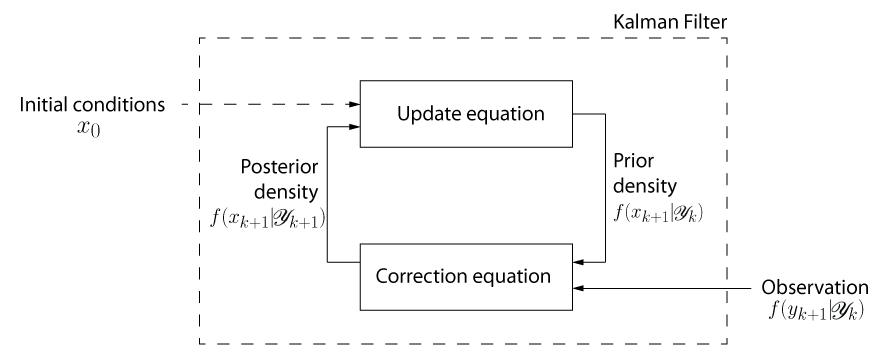
\includegraphics[width=.9\textwidth]{kalmanDiag.png}
	\caption{Ongoing Kalman filter cycle.}
\end{figure}

%Defining
%$$E[x_{k+1}|\filtrationObs{k}]=\hat{x}_{k+1}^-=\hat{x}_{k+1|k}$$
%$$E[x_{k}|\filtrationObs{k}]=\hat{x}_{k}^+=\hat{x}_{k|k}$$

%$$P_k^+=P_{k|k}=E[(x_k-\hat{x}_k^+)(x_k-\hat{x}_k^+)^T|\filtrationObs{k}]$$
%$$P_k^-=P_{k|k-1}=E[(x_k-\hat{x}_k^-)(x_k-\hat{x}_k^-)^T|\filtrationObs{k-1}]$$

The \emph{update equation} is responsible for projecting one step forward in time (in an unbiased fashion) the current state and error covariance estimates to obtain the prior estimates for the next time step.\\
\\
The \emph{correction equation} is responsible for incorporating a new measurement into the prior estimate to obtain the posterior estimate.\\
\\
The Kalman filter generates new state estimates as new observations becomes available, thus opening the possibility of real-time estimation. As a by-product, the filter generates the estimation error covariance matrix $P_{k+1}$, which measures the uncertainty in the estimate.
\\
%The Kalman filter estimates a process by using a form of feedback control. The filter estimates the process state at some time and then obtains feeback in the form of noisy observations. 

\begin{remark}
$P_k$ (and similarly $P_k^-$) can be seen as the covariance matrix of the posterior (prior) estimation error $e_k=x_k-\hat{x}_k$ (respectively $e_k^-=x_k-\hat{x}_k^-$), or the covariance matrix of the random variable $x_k$ conditioned on \filtrationObs{k}.
\end{remark}


%The Kalman filter recursively conditions the current estimate on all of the past measurements.

%Once such a conditional probability density function is propagated, the "optimal" estimate can be defined. Possible choices would include (i) the mean (ii) the mode or (iii) the median. A Kalman filter perfoms this conditional probability density propagation for problems in which the system can be described through a linear model and in which system and measurement noises are white and Gaussian. Under these three restrictions, the mean, mode and median coincide.

%the classical approach to doing this via model calibration typically requires that considerable amounts of data be collected and assimilated before the model can be used. 









\subsection{Application to Pair Trading}
To illustrate the use of the Kalman filter in a quantitative trading strategy setting, we will develop a short example inspired from \emph{statistical arbitrage} - see Dunis et al. (2010), Ajay Jasra (2011) or Helliott et al. (2005). \\

\emph{Pair trading} was pioneered by Gerry Bamberger and later by Nunzio Tartaglia's quantitative group at Morgan Stanley in the 1980s. The strategy involves forming a portfolio of two \emph{co-integrated} stocks whose relative pricing is away from its \emph{equilibrium} state. It is assumed that over time they will move back to a rational equilibrium (mean revert) and therefore weightning appropriately the number of stocks held should result in a profit which will be a function of the \emph{spread}.\\% (the difference between the two prices).\\
\\
We give the following preliminary definitions.
%(i. e. $E[|X_k|^2]< \infty$)
%\footnote{See lecture notes from  Bingham (2011).}
\begin{definition} A process $\{X_k\}$ is said to be \emph{strictly stationary}, if its finite-dimentional distributions are invariant under time-shifts - that is, for all $k \in \measure{N}$ and $\tau \in \measure{N}$ (called the \emph{lag}), $\{X_{k},...,X_{k+n}\}$ and $\{X_{k+\tau},...,X_{k+n+\tau}\}$ have the same distribution
\begin{equation*}
F(X_{k},...,X_{k+n})=F(X_{k+\tau},...,X_{k+n+\tau})
\end{equation*}
where $F(.)$ is the joint cumulative distribution function.
\end{definition}

%\begin{definition} A square integrable process $\{X_k\}$ (i. e. $E[|X_k|^2]< \infty$) is said to be \emph{weakly stationary} (or \emph{second-order stationary}), if for each $k \in N$,$E[X_k]$ and $Cov(X_k, X_{k+\tau})$ are independend of k.
%\end{definition}

%\footnotemark[\value{footnote}]
\begin{definition} A process $\{X_k\}$ is said to be \emph{weakly stationary}, if for each $k \in 
\measure{N}$, its mean $E[X_k]=\mu$ is constant over time and it covariance $Cov(X_k, X_{k+\tau})=\gamma(\tau)$ independs only on the lag $\tau$ and not on the time of $k$.
\end{definition}

\begin{remark}
Because only the first two moments of the stochastic process have to be defined and independent of the time, this process is also referred to as being \emph{second-order stationary} or \emph{covariance stationary}.
\end{remark}

\begin{remark}
A strictly stationary process is always weakly stationary. The converse is false in general but true for a normally distributed processes.
\end{remark}

We deduce that a stationary process has a clear tendency to return to a constant value over time (no trend).

\begin{definition} A process ${X_k}$ is said to be \emph{integrated of order one}, $I(1)$, if $\{X_k\}$ is non-stationary, but $\{ X_k-X_{k-1}\}$ is stationary.
\end{definition}

Introduced by Engle and Granger (1987), co-integration is a measure of the long-term dependencies in stochastic processes. 

\begin{definition}\footnote{See Banerjee et al. (2003) for a complete presentation.} Two processes $\{X_k\}$, $\{Y_k\}$ are said to be \emph{co-integrated} if they are both $I(1)$ and there exist $\beta \in \measure{R}$ such that the \emph{spread} $Y_k-\beta X_k$ is stationary in the weak sense.
\end{definition}

The figure below illustrate clearly co-integrated processes\footnote{Source data: http://finance.yahoo.com}, the two \emph{move} together.

\begin{figure}[h!]
	\centering
	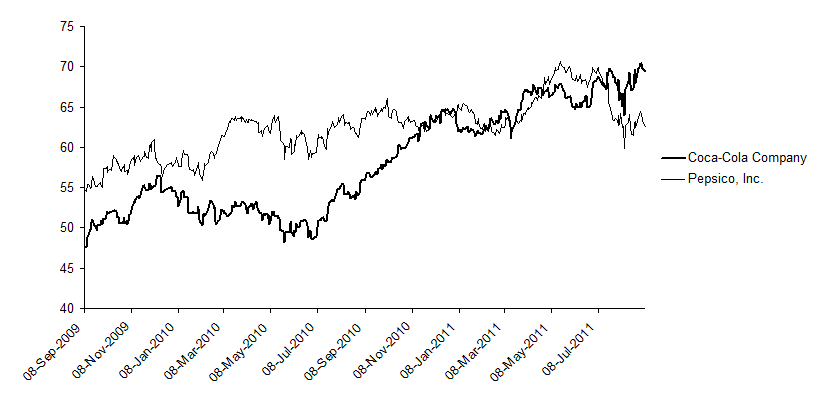
\includegraphics[width=.9\textwidth]{PepsiCoca.png}
	\caption{Adjusted daily closing prices of The Coca-Cola Company \\(NYSE: KO) and Pepsico, Inc. (NYSE: PEP) from 08-Sept-2011 to 06-Sept-2011.}
\end{figure}

\begin{remark}
Other potentially co-integrated pairs includes:\\
\begin{itemize}\itemsep0pt \addtolength{\itemsep}{-1\baselineskip}
\item Wal-Mart (WMT) and Target Corporation (TGT),\\
\item Dell (DELL) and Hewlett-Packard (HPQ),\\
\item Ford (F) and General Motors (GM).
\end{itemize}
\end{remark}
{\tiny .}
%\begin{figure}[h!]
%	\centering
%	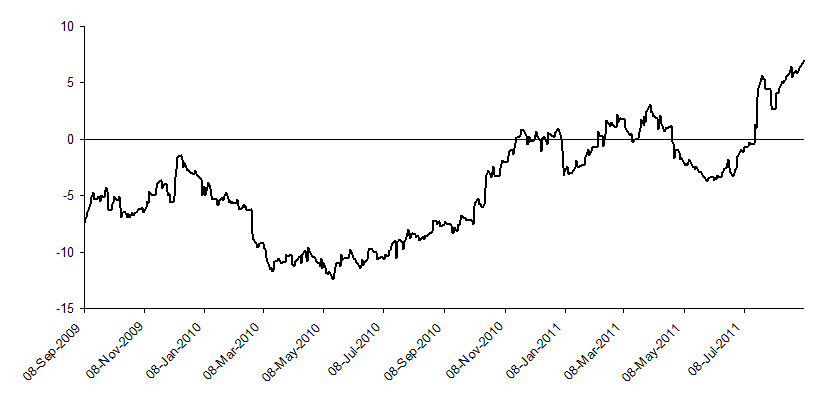
\includegraphics[width=.9\textwidth]{spreadPepsiCoca.png}
%	\caption{The spread is used to trigger buy or sell orders.}
%\end{figure}

The strategy consists of forming a corresponding pair of stocks $(x, y)$ from the same industry (as they face similar systematic risks) and then evaluate whether the pair is co-integrated in the sample period \footnote{The main methods of testing for co-integration are the \emph{Engle-Granger} (1987), the \emph{Johansen procedure} (1988,1991) and the \emph{Phillips-Ouliaris Cointegration Test}. These tests assume that the cointegrating vector remains constant during the period of study.}. \\
\\
Subsequently, the parameter $\beta$ is estimated using the Kalman filter given the following state-space model
\begin{align*}
\beta_{k+1}&=\beta_k+w_k\\
y_{k}&=x_k\beta_k+v_k
\end{align*}
where $v_k \sim N(0, P)$ and $w_k \sim N(0, Q)$ are independent Gaussian white noises.\\
\\
Following Theorem \ref{thm:kalman}, the solution is given by
\begin{equation*}
\hat{\beta}_{k+1}=\hat{\beta}_{k}+K_{k+1}(y_{k+1}-x_k\hat{\beta}_k)
\end{equation*}

\begin{equation*}
P_{k+1}=(I-K_{k+1}x_{k+1})P^-_{k+1}
\end{equation*}
where the Kalman gain is 
\begin{equation*}
K_{k+1}=P^-_{k+1}x_{k+1}^T(x_{k+1}P^-_{k+1}x_{k+1}^T+R)^{-1}
\end{equation*}
and
\begin{equation*}
P^-_{k+1}=P_k+Q.
\end{equation*}

\begin{figure}[h!]
	\centering
	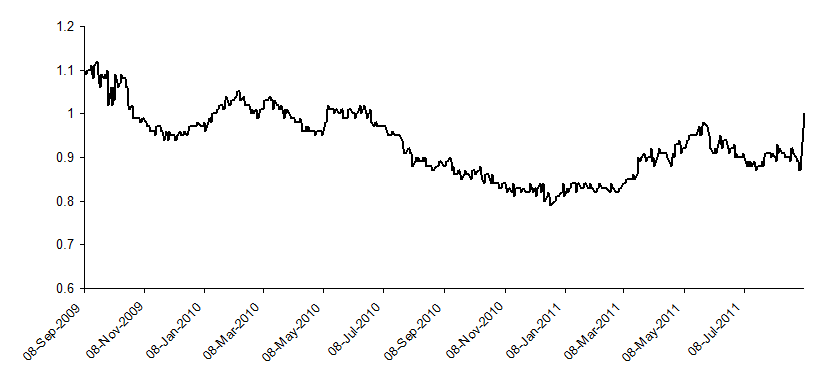
\includegraphics[width=.9\textwidth]{beta.png}
	\caption{Estimated $\beta_k$ of The Coca-Cola Company \\(NYSE: KO) and Pepsico, Inc. (NYSE: PEP) from 08-Sept-2011 to 06-Sept-2011. \\$Q=0.003$, $R=1$, $\beta_0=1$ and $P_0=1$.\\(See appendix \ref{app:pairTrading} for the source code.)}
\end{figure}

%\footnote{See appendix \ref{app:pairTrading} form the source code.}

%$Q=cov(w_k)$ and $R=cov(v_k)$ can be estimated using the maximum likelihood.\\


\begin{tabbing}Bec\=ause of its stationarity, the spread will mean revert to a constante $\mu$ over time:\\
\> (i) if $y_k-\beta_k x_k>\mu$ buy $\beta_k$ of $x_k$ and short-sell one unit of $y_k$,\\
\>(ii) if $y_k-\beta_k x_k<\mu$ buy one unit of $y_k$ and short-sell $\beta_k$ of $x_k$.\\
\end{tabbing}

This strategy is \emph{market neutral} meaning that it is profitable regardless of the market price direction. \\
\\
However simplistic this strategy seems to be at first glance, it requires leverage to be truly profitable. And if the mean revertion rate is not high enough, the position will be too costly to hold on to.
\\
%How do we find co-integrated stocks?







%\subsection{The Kalman Filter with Correlated Noises}
%So far, our derivation of the Kalman filter assumed that the process noise $w_k$ and measurement noise $v_k$ were uncorrelated - that is we assumed that $E[w_kv_k^T]=0$ for all $k$. We will show how correlated process and measurement noise changes the Kalman filter equations.
%Suppose that we have a system given by 


%See Ma et al.(), D. Simon (2006) or Dover et al. (1979) (p105).


%\begin{equation}
%E\left( \begin{bmatrix}w_k\\ v_k\\x_0 \end{bmatrix} 
%\begin{bmatrix}w_k^T & v_k^T & x_0^T & 1 \end{bmatrix} \right)
%=\begin{bmatrix}
%Q_k & S_k & 0 & 0\\ 
%S_k^T & R_k & 0 & 0\\
%0 & 0 & P_0 & x_0
%\end{bmatrix}
%\end{equation}


%\begin{remark}
%One obtains the equations encountered earlier by setting $S_k=0$.
%\end{remark}

%~Later we will relax (). 







\newpage
\section{Drift Estimation Problem and the Kalman Filter}\label{sec:app}
%\subsection{Statistical Parameters Estimation}
We recall from the risk-neutral analysis in chapter \ref{sec:riskn} that our objective is to estimate the unknown drift function
\begin{equation}
\mu_k=(r-q)+\lambda_k\sigma
\end{equation}
where
\begin{equation}
\lambda_{k+1} = \lambda_k + \kappa(\bar{\lambda}-\lambda_k)\Delta t +\sigma_\lambda \Delta W.
\end{equation}
We say that the drift function $\mu_k$ is \emph{parametric} and we are left with four parameters (see table \ref{table:params}) that we need to estimate in order to recover $\mu_k$ from the observations.
\begin{table}[h!]
  \begin{center}
    \begin{tabular}{ c p{3cm} p{5cm} }
    \hline
		Parameter & Framework & Estimation Method\\ \hline
		$\lambda_k$ & Bayesian & Kalman filter\\
		%$\sigma$ & Model based & Implied volatility \\ %Newton's Method
		$\kappa,\bar{\lambda},\sigma_\lambda$ & Classical & Maximum likelihood\\ %$\theta=(\kappa,\bar{\lambda},\sigma_\lambda)$
    \hline
    \end{tabular}
  \end{center}
  \caption{Parameter Estimation.}\label{table:params}
\end{table}

In this section we will make use of the Kalman filter derived in chapter \ref{sec:kalmanFilter} to estimate $\lambda_k$. The remaining parameters $\kappa,\bar{\lambda}$ and $\sigma_\lambda$ will be estimated in chapter \ref{sec:est} using the \emph{maximum likelihood estimator}.








\subsection{The State-Space Equations}
In order to cast equation \eqref{eq:sys4} into the \textit{state space} model \eqref{eq:linstate} and \eqref{eq:linobs}, we observe from equation \eqref{eq:deltaW} that $\Delta W =\sqrt{\Delta t}.\epsilon$ where $\epsilon \sim N(0,1)$. Therefore equations \eqref{eq:sys4} can be written

%\begin{equation}
%\begin{matrix}
%	\begin{array}{lcrcrcr}
%		\lambda_{k+1} & = & \lambda_k &+& \kappa(\bar{\lambda}-\lambda_k)\Delta t & + & \sigma_\lambda \sqrt{\Delta} \\
%	\end{array}\\
%	\left\{ \begin{array}{lcrcrcr}
%				s_{k+1} & = & s_k &+& (r-q+\sigma\lambda_k-\frac{\sigma^2}{2}) \Delta t & + & \sigma  \sqrt{\Delta t}.\epsilon \\ 
%				f_{k+1} & = & f_k &+& (\sigma\lambda_k-\frac{\sigma^2}{2}) \Delta t & + & \sigma  \sqrt{\Delta t}.\epsilon \\ 
%				c_{k+1} & = & c_k &+& (r+\sigma_c\lambda_k-\frac{\sigma_c^2}{2})\Delta t &+& \sigma_c \sqrt{\Delta t}.\epsilon \\
%	        \end{array} \right. 
%\end{matrix}
%\end{equation}

\begin{equation}\label{eq:sys5}
\left\{ \begin{array}{lcrcrcr}
			\lambda_{k+1} & = & \lambda_k &+& \kappa(\bar{\lambda}-\lambda_k)\Delta t & + & \sigma_\lambda \sqrt{\Delta t}.\epsilon_k\\
			s_{k+1} & = & s_k &+& (r-q+\sigma\lambda_k-\frac{\sigma^2}{2}) \Delta t & + & \sigma  \sqrt{\Delta t}.\epsilon_k \\ 
			f_{k+1} & = & f_k &+& (\sigma\lambda_k-\frac{\sigma^2}{2}) \Delta t & + & \sigma  \sqrt{\Delta t}.\epsilon_k \\ 
			c_{k+1} & = & c_k &+& (r+\sigma_c\lambda_k-\frac{\sigma_c^2}{2})\Delta t &+& \sigma_c \sqrt{\Delta t}.\epsilon_k 
        \end{array} \right. .
\end{equation}







\subsubsection{The State Transition Equation}

%Writting $X_k=\lambda_k$ and and $\Delta W =\sqrt{\Delta t}.\epsilon$ where $\epsilon \sim N(0,1)$, the equation () gives us
%\begin{align*}
%X_{k+1} &=X_k+\kappa(\bar{\lambda}-X_k)\Delta t+\sigma_\lambda \Delta W %\notag\\
%&=\kappa \bar{\lambda} \Delta t+(1-\kappa \Delta t)Y_n+\sigma_\lambda \sqrt{\Delta t}\epsilon\\
%&= a+BX_k+R\epsilon_k \text{(State Transition Equation)}
%\end{align*}
Writting $X_k=\lambda_k$ for the state variable, the equation (\ref{eq:sys5}a) gives us the \textit{state transition equation}
\begin{equation}\label{eq:driftstate}
\boxed{X_{k+1}= a+BX_k+R\epsilon_k} %\text{(State Transition Equation)}
\end{equation}
where %$a=\kappa \bar{\lambda} \Delta t$, $B=1-\kappa \Delta t$, $R=\sigma_\lambda \sqrt{\Delta t}$.
\begin{equation}
\left\{ \begin{array}{ll}
          a & = \kappa \bar{\lambda} \Delta t \\ 
          B & = 1-\kappa \Delta t \\ 
          R & = \sigma_\lambda \sqrt{\Delta t}
        \end{array} \right. 
\end{equation}
are scalar constants.






\subsubsection{The Observation Equation}
There are three different observations related to the same state variable $X_k$ namely 
\begin{equation}
\left\{ \begin{array}{lcrcrcr}
			\Delta s_{k} & = & (r-q-\frac{\sigma^2}{2}) \Delta t & + & \sigma \Delta t X_k & + & \sigma  \sqrt{\Delta t}.\epsilon_k \\ 
			\Delta f_{k} & = & -\frac{\sigma^2}{2} \Delta t & + & \sigma \Delta t X_k & + & \sigma  \sqrt{\Delta t}.\epsilon_k \\ 
			\Delta c_{k} & = & (r-\frac{\sigma_c^2}{2})\Delta t & + & \sigma_c \Delta t X_k & + & \sigma_c \sqrt{\Delta t}.\epsilon_k 
        \end{array} \right. .
\end{equation}
As a result, we will allow for a vector valued observation $Y$ such that
\begin{equation}
Y_k=d_k+D_kX_k+H_k\epsilon_k
\end{equation}
where
\begin{equation}
Y_k=\begin{bmatrix}
\Delta s_k\\ 
\Delta f_k\\ 
\Delta c_k
\end{bmatrix}, 
d_k=\begin{bmatrix}
(r-q-\frac{\hat{\sigma_k}^2}{2})\Delta t\\ 
-\frac{\hat{\sigma_k}^2}{2}\Delta t\\ 
(r-\frac{\hat{\sigma_{c,k}}^2}{2})\Delta t
\end{bmatrix},
H_k=\begin{bmatrix}
\hat{\sigma_k}\sqrt{\Delta t}\\ 
\hat{\sigma_k}\sqrt{\Delta t}\\ 
\hat{\sigma_{c,k}}\sqrt{\Delta t}
\end{bmatrix},
D_k=H_k\sqrt{\Delta t}.
\end{equation}

%(Financial_Econometrics_Modeling__Market_Microstructure__Factor_Models_and_Financial_Risk_Measures.pdf)
%The availability of large, high-frequency financial data sets potentially provides a rich source of information about  asset-price dynamics. Intra-daily return data have the potential to provide very accurate estimates of the underlying. These  measures, however, have been shown to be sensitive to market microstructure noise inherent in the observed asset prices. 
In addition to the system noise $\epsilon_k$, we will also assume the existance of a \textit{market microstructure noise} term $Q_k\eta_k$ where $\eta_k \sim N(0,1)$. The market microstructure noise arise from the impact that the financial intermediaries linking buyers and sellers (such as brokers, market makers, ...) has on the market. These market participants are subject to certain rules that each exchange and national legislation impose on them, called the \textit{market structure}. The market structure affects the price formation process both spatially and temporally in the form of bid-ask spread and nonsynchronicity of observed data. An introduction to the general idea of market microstructure can be found in O'Hara (1997). Although the structural forms of financial markets are different around the world, we will follow Bhar, Chiarella and Runggaldier (2004) and assumed a weigtning factor of the form $Q_k = \begin{bmatrix} 0.001\\ 0.001\\ 0.001 \end{bmatrix}$ which reflects a typical bid-ask spread.

Consequently, the observation equation can be written
\begin{equation}\label{eq:driftobs}
\boxed{Y_k=d_k+D_kX_k+v_k}
\end{equation}
where
\begin{equation}
v_k=H_k\epsilon_k+Q_k\eta_k.
\end{equation}
\begin{remark}\label{rem:corrnoise}
We observe that we are in the case where there is correlation between the system noise and observation noise
\footnote{For two matrices A and B we have the following properties of transpose: $(A+B)^T=A^T+B^T$ and $(AB)^T=B^TA^T.$}
\begin{equation}
%\m{G}_k=E[\m{\epsilon}_k\m{v}_k^T]=\begin{bmatrix} H_k^1 & H_k^2 & H_k^3 \end{bmatrix}
G_k=E[\m{\epsilon}_k\m{v}_k^T]=\begin{bmatrix} \hat{\sigma_k}\sqrt{\Delta t} & \hat{\sigma_k}\sqrt{\Delta t} & \hat{\sigma_{c,k}}\sqrt{\Delta t} \end{bmatrix}=H_k^T.
\end{equation}
\end{remark}









\subsection{The Kalman Filtering Solution}
We introduce the following common notations used by Bhar, Chiarella and Runggaldier (2004) - see table 2, along with the parameters dimension - see table 3.
\begin{table}[h!]
  \begin{center}
    \begin{tabular}{ l l p{8.3cm} }
    \hline
		 &  & Definition\\ \hline
		$X_{i|j}$ & $E[X_{i}|\filtrationObs{j}]$ & Expectation of $X_{i}$ based on observations up to time $j$.\\
		$P_{i|j}$ & $cov(X_{i}|\filtrationObs{j})$ & Covariance of $X_i$ based on observations up to time $j$.\\
		$F_{k+1}$ & $cov(y_{k+1}|\filtrationObs{k})$ & Covariance of the observations.\\
%		$X_{k+1|k}$ & $E[X_{k+1}|\filtrationObs{k}]$ & Expectation of $X_{k+1}$ based on observations up to time k.\\
%		$X_{k+1|k+1}$ & $E[X_{k+1}|\filtrationObs{k+1}]$ & Expectation of $X_{k+1}$ based on observations up to time k+1.\\
%		$X_{k|k}$ & $E[X_{k}|\filtrationObs{k}]$ & Expectation of $X_{k}$ based on observations up to time k.\\
%		$P_{k+1|k}$ & $cov(X_{k+1}|\filtrationObs{k})$ & \\
%		$P_{k+1|k+1}$ & $cov(y_{k+1}|\filtrationObs{k+1})$ & \\
%		$F_{k+1}$ & $cov(y_{k+1}|\filtrationObs{k})$ & \\
    \hline
    \end{tabular}
  \end{center}
  \caption{Summary of the notations.}
\end{table}

\begin{table}[h!]
  \begin{center}
    \begin{tabular}{ p{6cm} p{3cm}}
    \hline
		Parameter & Dimension\\ \hline
		$X_{k|k}$, $X_{k+1|k}$, $X_{k+1|k+1}$, \\$P_{k+1|k}$, $P_{k+1|k+1}$, \\$a_k$, $B$, $R$, $\epsilon_k$, $\eta_k$ & 1x1\\ \hline
		$P^{yx}_k$, $Y_k$, $d_k$, $H_k$, $D_k$, $v_k$, $Q_k$, $\theta$ & 3x1\\ \hline
		$P^{xy}_k$, $G_k$, $K_{k}$ & 1x3\\ \hline
		$F_k, V_k$ & 3x3\\
    \hline
    \end{tabular}
  \end{center}
  \caption{Parameters dimension.}
\end{table}


The Kalman filter solution for the state-space equations \eqref{eq:driftstate} and \eqref{eq:driftobs} described above is summarized in the following theorem.

\begin{thm}\label{thm:driftKal}
The optimal filter for the state space \eqref{eq:driftstate}, \eqref{eq:driftobs} consists of the \emph{update equations}
\begin{equation}
\left\{ \begin{array}{ll}
			X_{k+1|k}=a+BX_{k|k}\\
			P_{k+1|k}=BP_{k|k}B^T+RR^T
        \end{array} \right. 
\end{equation}
and the \emph{correction equations}
\begin{equation}
\left\{ \begin{array}{ll}
			X_{k+1|k+1}&=X_{k+1|k}+K_{k+1}(Y_{k+1}-D_{k+1}X_{k+1|k}-d_{k+1})\\
			P_{k+1|k+1}&=(1-K_{k+1}D_{k+1})P_{k+1|k}+K_{k+1}G^T_{k+1}R
        \end{array} \right. 
\end{equation}
where
\begin{equation}
			K_{k+1}=(P_{k+1|k}D^T_{k+1}+RG_{k+1})F^{-1}_{k+1}
\end{equation}
is the Kalman gain and			
\begin{equation}
F_{k+1}=D_{k+1}P_{k+1|k}D_{k+1}^T+D_{k+1}RG_{k+1}+G_{k+1}^TR^TD_{k+1}^T+H_{k+1}H_{k+1}^T+Q_{k+1}Q_{k+1}^T
\end{equation}
is the covariance of the observations provided that $F^{-1}_{k+1}$ exists\footnote{We may replace $F^{-1}_{k+1}$ by its pseudo-inverse.}.
\end{thm}



\begin{proof}
The proofs of the Kalman filter provided in the chapter \ref{sec:kalmanFilter} assumed uncorelation between the model and the observation noises. Therefore following remark \ref{rem:corrnoise}, we need to derive theorem \ref{thm:driftKal} taking into account this new fact.\\
%\begin{equation}
%P(X_{k+1}|\filtrationObs{k+1}) = \frac{P(Y_{k+1}|X_{k+1})P(X_{k+1}|\filtrationObs{k})}{P(Y_{k+1}|\filtrationObs{k})} .
%\end{equation} 
\\
Following section \ref{proof:kal2}, we need to identify the three density functions $P(Y_{k+1},X_{k+1}|\filtrationObs{k})$, $P(X_{k+1}|\filtrationObs{k})$ and $P(Y_{k+1}|\filtrationObs{k})$ in order to recover $P(X_{k+1}|\filtrationObs{k+1})$ from lemma \ref{lem:kal2}.

%The prior density of $X_{k+1}$ is given by
(i) The update density is defined as
$$P(X_{k+1}|\filtrationObs{k})=N(X_{k+1|k},P_{k+1|k})$$
with the expectation given by
\begin{align*}
X_{k+1|k}&=E[X_{k+1}|\filtrationObs{k}]\\
&=a+BE[X_k|\filtrationObs{k}]\\ 
&=a+BX_{k|k}.
\end{align*}
The variance is given by
\begin{align*}
P_{k+1|k}&=E[(X_{k+1}-X_{k+1|k})(X_{k+1}-X_{k+1|k})^T|\filtrationObs{k}]\\
\end{align*}
with 
\begin{align*}
X_{k+1}-X_{k+1|k}&=(a+BX_k+R\epsilon_k)-(a+BX_{k|k})\\
&=B(X_k-X_{k|k})+R\epsilon_k.
\end{align*}
Therefore
\begin{align*}
P_{k+1|k}=&E[B(X_k-X_{k|k})(B(X_k-X_{k|k}))^T|\filtrationObs{k}]+\\
&E[B(X_k-X_{k|k})(R\epsilon_k)^T|\filtrationObs{k}]+\\
&E[(R\epsilon_k)(B(X_k-X_{k|k}))^T|\filtrationObs{k}]+\\
&E[(R\epsilon_k)(R\epsilon_k)^T|\filtrationObs{k}]\\
%
=&BE[(X_k-X_{k|k})(X_k-X_{k|k})^T|\filtrationObs{k}]B^T+\\
&BE[(X_k-X_{k|k})\epsilon_k^T|\filtrationObs{k}]R^T+\\
&RE[\epsilon_k(X_k-X_{k|k})^T|\filtrationObs{k}]B^T+\\
&RE[\epsilon_k\epsilon_k^T|\filtrationObs{k}]R^T.\\
\end{align*}

Observing that, $$E[(X_k-X_{k|k})(X_k-X_{k|k})^T|\filtrationObs{k}]=P_{k|k},$$ 
$$E[(X_k-X_{k|k})\epsilon_k^T|\filtrationObs{k}]=0,$$
$$E[\epsilon_k(X_k-X_{k|k})^T|\filtrationObs{k}]=0,$$
$$E[\epsilon_k\epsilon_k^T|\filtrationObs{k}]=1.$$
We get
\begin{equation*}
P_{k+1|k}=BP_{k|k}B^T+RR^T.
\end{equation*}
\\
(ii) The observation density is given by
$$P(Y_{k+1}|\filtrationObs{k})=N(E[Y_{k+1}|\filtrationObs{k}],F_{k+1})$$
with expectation given by
\begin{align*}
E[Y_{k+1}|\filtrationObs{k}]&=d_{k+1}+D_{k+1}E[X_{k+1}|\filtrationObs{k}]\\
&=d_{k+1}+D_{k+1}X_{k+1|k}.
\end{align*}
The variance is given by
\begin{align*}
F_{k+1}=E[(Y_{k+1}-Y_{k+1|k})(Y_{k+1}-Y_{k+1|k})^T|\filtrationObs{k}]
\end{align*}
with 
\begin{align*}
Y_{k+1}-Y_{k+1|k}&=(d_{k+1}+D_{k+1}X_{k+1}+v_{k+1})-(d_{k+1}+D_{k+1}X_{k+1|k}+E[v_{k+1}|\filtrationObs{k}])\\
&=D_{k+1}(X_{k+1}-X_{k+1|k})+v_{k+1}.
\end{align*}
Therefore
\begin{align*}
F_{k+1}=&E[D_{k+1}(X_{k+1}-X_{k+1|k})(D_{k+1}(X_{k+1}-X_{k+1|k}))^T|\filtrationObs{k}]+\\
&E[D_{k+1}(X_{k+1}-X_{k+1|k})v_{k+1}^T|\filtrationObs{k}]+\\
&E[v_{k+1}(D_{k+1}(X_{k+1}-X_{k+1|k}))^T|\filtrationObs{k}]+\\
&E[v_{k+1}v_{k+1}^T|\filtrationObs{k}]\\
%
=&D_{k+1}E[(X_{k+1}-X_{k+1|k})(X_{k+1}-X_{k+1|k})^T|\filtrationObs{k}]D_{k+1}^T+\\
&D_{k+1}E[(X_{k+1}-X_{k+1|k})v_{k+1}^T|\filtrationObs{k}]+\\
&E[v_{k+1}(X_{k+1}-X_{k+1|k})^T|\filtrationObs{k}]D_{k+1}^T+\\
&E[v_{k+1}v_{k+1}^T|\filtrationObs{k}]
\end{align*}
with
%\begin{align*}
%E[(X_{k+1}-X_{k+1|k})(X_{k+1}-X_{k+1|k}))^T|X_k]=P_{k+1|k}
%\end{align*},
\begin{align*}
E[v_{k+1}v_{k+1}^T|\filtrationObs{k}]=&E[(H_{k+1}\epsilon_{k+1}+Q_{k+1}\eta_{k+1})(H_{k+1}\epsilon_{k+1}+Q_{k+1}\eta_{k+1})^T|\filtrationObs{k}]\\
=&H_{k+1}E[\epsilon_{k+1}\epsilon_{k+1}^T|\filtrationObs{k}]H_{k+1}^T+\\
&H_{k+1}E[\epsilon_{k+1}\eta_{k+1}^T|\filtrationObs{k}]Q_{k+1}^T+\\
&Q_{k+1}E[\eta_{k+1}\epsilon_{k+1}^T|\filtrationObs{k}]H_{k+1}^T+\\
&Q_{k+1}E[\eta_{k+1}\eta_{k+1}^T|\filtrationObs{k}]Q_{k+1}^T+\\
%
=&H_{k+1}H_{k+1}^T+Q_{k+1}Q_{k+1}^T\\
\end{align*}
and
\begin{align*}
E[(X_{k+1}-X_{k+1|k})v_{k+1}^T|\filtrationObs{k}] &= E[(B(X_k-X_{k|k})+R\epsilon_k)v_{k+1}^T|\filtrationObs{k}]\\
%&=B(E[X_k|X_k]-X_{k|k})+RE[\epsilon_k|X_k]\\
&=RE[\epsilon_kv_{k+1}^T|\filtrationObs{k}]=RG_{k+1}.
\end{align*}

%\begin{align*}
%E[X_{k+1}-X_{k+1|k}|X_k] &= E[B(X_k-X_{k|k})+R\epsilon_k|X_k] from ()\\
%&=B(E[X_k|X_k]-X_{k|k})+RE[\epsilon_k|X_k]\\
%&=RE[\epsilon_k|X_k]
%\end{align*}
%(computed earlier in update equations)

Combining gives
\begin{align*}
F_{k+1}
%=&D_{k+1}P_{k+1|k}D_{k+1}^T+\\
%&D_{k+1}E[R\epsilon_k v_{k+1}^T|X_k]+\\
%&E[v_{k+1}(R\epsilon_k)^T|X_k]D_{k+1}^T+\\
%&H_{k+1}H_{k+1}^T+Q_{k+1}Q_{k+1}^T\\
%
%=&D_{k+1}P_{k+1|k}D_{k+1}^T+\\
%&D_{k+1}RE[\epsilon_k v_{k+1}^T|X_k]+\\
%&E[v_{k+1}\epsilon_k^T|X_k]R^TD_{k+1}^T+\\
%&H_{k+1}H_{k+1}^T+Q_{k+1}Q_{k+1}^T\\
%
=&D_{k+1}P_{k+1|k}D_{k+1}^T + D_{k+1}RG_{k+1} + G_{k+1}^TR^TD_{k+1}^T + H_{k+1}H_{k+1}^T+Q_{k+1}Q_{k+1}^T.
\end{align*}

(iii) The joint density of the state and observation at time $k+1$ given prior knowledge is
$$P(X_{k+1}, Y_{k+1}|\filtrationObs{k})$$%=N(E[Y_{k+1}|\filtrationObs{k}],F_{k+1})$$

%For $P_{k+1}^{xy}$
%P_{k+1}^{xy}
\begin{align*}
cov(X_{k+1}, Y_{k+1}|\filtrationObs{k})&=E[(X_{k+1}-X_{k+1|k})(Y_{k+1}-Y_{k+1|k})^T|\filtrationObs{k}]\\
&=E[(X_{k+1}-X_{k+1|k})(D_{k+1}(X_{k+1}-X_{k+1|k})+v_{k+1})^T|\filtrationObs{k}]\\
&=E[(X_{k+1}-X_{k+1|k})((X_{k+1}-X_{k+1|k})^TD_{k+1}^T+v_{k+1}^T)|\filtrationObs{k}]\\
&=P_{k+1|k}D_{k+1}^T+E[(X_{k+1}-X_{k+1|k})v_{k+1}^T|\filtrationObs{k}]\\
&=P_{k+1|k}D_{k+1}^T+RG_{k+1}
\end{align*}

(iv) We finally deduce the transpose of the covariance of the joint density $P(X_{k+1}, Y_{k+1}|\filtrationObs{k})^T$,

%For $P_{k+1}^{yx}$
%\begin{align*}
%P_{k+1}^{yx}=\left(P_{k+1}^{xy}\right)^T=D_{k+1}P_{k+1|k}^T+R^TG_{k+1}^T
%\end{align*}

\begin{align*}
cov(X_{k+1}, Y_{k+1}|\filtrationObs{k})^T=D_{k+1}P_{k+1|k}^T+R^TG_{k+1}^T.
\end{align*}

%For $P_{k+1}^{xx}$
%\begin{align*}
%P_{k+1}^{xx}=P_{k+1|k}
%\end{align*}
(v) Making use of lemma \eqref{lem:kal2} complete the proof.
\end{proof}








%\subsection{reconciliation}


%\textbf{Proposition}: Conditional multivariate normal distribution\\
%If X and Y are two jointly normal vectors of respective dimensions $p$ and $q$ with $p+q=n$
%$$P(X,Y)=N\left(
%\begin{bmatrix} \bar{X}\\ \bar{Y} \end{bmatrix}
%, \begin{bmatrix}
%P_{xx} & P_{xy}\\ 
%P_{yx} & P_{yy}
%\end{bmatrix}\right)$$
%then 
%$$P(X|Y)=N\left( \bar{X}+P_{xy}P_{yy}^{-1}(Y-\bar{Y}), P_{xx}-P_{xy}P_{yy}^{-1}P_{yx} \right).$$
%\textbf{Proof}: See proof in the appendix.
%\\
%\\
%The joint distribution of the update $X$ and the observation $Y$ at $k+1$ is given by
%$$P(X_{k+1},Y_{k+1})=N\left(
%\begin{bmatrix} X_{k+1|k}\\ Y_{k+1|k} \end{bmatrix}
%, \begin{bmatrix}
%P^{xx}_{k+1} & P^{xy}_{k+1}\\ 
%P^{yx}_{k+1} & P^{yy}_{k+1}
%\end{bmatrix}\right).$$
%According to Theorem x (see proof in the appendix), it follows that the posterior density of $X_{k+1}$ given the observation vector $\mathbf{Y}_{k+1}$ is 
%$$P(X_{k+1}|Y_{k+1})=N(X_{k+1|k+1},P_{k+1|k+1})$$
%$$X_{k+1|k+1}=X_{k+1|k}+P^{xy}_{k+1}(P^{yy}_{k+1})^{-1}(Y_{k+1}-Y_{k+1|k})$$
%$$P_{k+1|k+1}=P^{xx}_{k+1}+P^{xy}_{k+1}(P^{yy}_{k+1})^{-1}P^{yx}_{k+1}$$
%where
%\begin{equation}
%\boxed{
%	\left\{ \begin{array}{ll}
%	          X_{k+1|k+1}&=X_{k+1|k}+P^{xy}_{k+1}(P^{yy}_{k+1})^{-1}(Y_{k+1}-Y_{k+1|k}) \\ 
%	\\
%	          P_{k+1|k+1}&=P^{xx}_{k+1}-P^{xy}_{k+1}(P^{yy}_{k+1})^{-1}P^{yx}_{k+1}.
%	        \end{array} \right. 
%}
%\end{equation}








\subsection{Discussion}
%It is important to ask what, if anything, can be gained from fitering the data. Can the state be determined from the data? It turns out that the answer to this question is related to the system model itself. If little is gained from filtering, then we should consider remodeling the system. How well the state is known is measure by the estimation error covariance matrix $P$.

It is important to ask what, if anything, can be gained from fitering the data. How well the state is known is measured by the estimation error covariance $P_{k+1|k}=E[(X_{k+1}-X_{k+1|k})(X_{k+1}-X_{k+1|k})^T|\filtrationObs{k}]$. If little is gained from filtering, then we should consider remodeling the system \eqref{eq:sys4}. It should be noted that $P_{k+1|k}$ also depends on the initial condition $P_0$ and does not reflect the uncertainty in the estimate of the filtering alone.








\newpage
\section{Parameter Estimation using Maximum Likelihood}\label{sec:est}
We have discussed Bayesian estimators in section \ref{sec:opfilt}. We will show in this section that the non-time-dependent parameters $\theta=\begin{bmatrix} \kappa & \bar{\lambda} & \sigma_\lambda \end{bmatrix}$ can be estimated using the \emph{Maximum Likelihood Estimator }(MLE).\\ 

Contrary to Bayesian estimators where the parameters are regarded as random variables, in non-Bayesian setting the sought paramters are considered as fixed and the \emph{Maximum Likelihood Estimator} (MLE) is a common choice of estimator.

%With parametric estimation, the parameters are no longer regarded as random variables. Instead, the sought parameters are regarded as fixed but unknown. 

% In a non-Bayesian setting (i.e. when the paramters are considered as fixed and not random variables) the \emph{Maximum Likelihood Estimator} (MLE) is a common choice.

%$\theta=(\kappa,\bar{\lambda},\sigma_\lambda)$ 
\begin{definition}
The \emph{likelihood function} is given by
\begin{equation}
L(\theta)=P(y|\theta)
\end{equation}
where $P(\theta|y)$ is regarded as a function of the parameters $\theta$.

\end{definition}

\begin{definition}
The maximum likelihood estimator $\hat{\theta}_{ML}$ is the estimator that maximizes the likelihood function $L(\theta)$
\begin{equation}
\hat{x}_{ML}(y)=\arg\max_{\theta} L(\theta)
\end{equation}
\end{definition}
{\tiny .}
%The likelihood function is the basis for Bayesian statistics.  

\begin{remark}
As for the \emph{Maximum a Posteriori} (MAP), the MLE estimator need not exist nor be unique.
\end{remark}
{\tiny .}

Therefore given the observations $\filtrationObs{N}$, the parameter vector $\theta$ corresponding to the density most likely generating the observation is chosen. \\
\\
We recall that the observations $Y_i$ are independent and normally distributed (i.e. $Y\sim N(Y_{k+1|k},F_{k+1})$). The likelihood function is given by
\begin{align*}
L(\theta)&=P(\theta|\filtrationObs{N})=P(\theta|Y_1)\cdots P(\theta|Y_{N})=\prod_{k=0}^{N-1}P(\theta|Y_{k+1})\\%\\
&=\prod_{k=0}^{N-1}\frac{1}{(2\pi)^{3/2}|F_{k+1}|^{1/2}}e^{-\frac{1}{2}(Y_{k+1}-Y_{k+1|k})^TF_{k+1}^{-1}(Y_{k+1}-Y_{k+1|k})}\\
&=\frac{1}{(2\pi)^{3N/2}}\prod_{k=0}^{N-1}\frac{1}{|F_{k+1}|^{1/2}}e^{-\frac{1}{2}(Y_{k+1}-Y_{k+1|k})^TF_{k+1}^{-1}(Y_{k+1}-Y_{k+1|k})}.
\end{align*}

Maximizing the logarithm of the likelihood function (called \textit{log-likelihood}) is equivalent to maximizing the likelihood function as log(.) is monotonous, therefore
\begin{align*}
l(\theta)=log(L(\theta))&=-\frac{3N}{2}log(2\pi) + \sum_{k=0}^{N-1}log\left( \frac{1}{|F_{k+1}|^{1/2}}e^{-\frac{1}{2}(Y_{k+1}-Y_{k+1|k})^TF_{k+1}^{-1}(Y_{k+1}-Y_{k+1|k})} \right)\\
%
&=-\frac{3N}{2}log(2\pi) + \sum_{k=0}^{N-1}\left( -\frac{1}{2}log|F_{k+1}|-\frac{1}{2}(Y_{k+1}-Y_{k+1|k})^TF_{k+1}^{-1}(Y_{k+1}-Y_{k+1|k}) \right) \\
%
&=-\frac{3N}{2}log(2\pi) - \frac{1}{2}\sum_{k=0}^{N-1}log|F_{k+1}|-\frac{1}{2}\sum_{k=0}^{N-1}(Y_{k+1}-Y_{k+1|k})^TF_{k+1}^{-1}(Y_{k+1}-Y_{k+1|k}).
\end{align*}
%With $Y_{k+1}-Y_{k+1|k}=D_{k+1}(X_{k+1}-X_{k+1|k})+v_{k+1}$ (see ())
The standard analytical method of finding the MLE is to take the first partial derivatives of the
log-likelihood with respect to each parameter $\theta_i$. Therefore from here, we will resort to numerical methods to find the roots of $\frac{\partial l}{\partial \theta_i}$ and deduce the best approximation of $\hat{\theta}_{ML}$.




%% REAL DATA SECTION
%\newpage
%\section{Misc.}
%\subsubsection{Continuous Contracts}
%Forward and Option markets are comprised of individual contracts, each with a pre-determined life-span. At any stage, the market consists of a number of contracts, or "delivery months", that have expiry dates stretching out into the future. As one contract expires, another is listed for trading, and so the cycle continues. The only way that a long-term continuous history of Soyoil prices can be examined is to access a record of cash market prices.

%It is possible to join the individual contracts together in a way as to represent their history. But it must be borne in mind that the result will merely be a representation of that history, or a computation, that is handled by a particular algorithm.

%S\&P500 index: a common proxy for the market portfolio
%The  average  real  return  on  six-month commercial paper, a proxy for the risk-free interest rate










\newpage
\section{Discussion}


%According to Girsanov's theorem, $\lambda(t)$ is the link between the market measure \measure{P} and the risk-neutral measure \measure{Q}. 

%Assumptions: parametric form/risk-neutral/r=cst/$\sigma$=cst/Uniformly spaced time intervals will be assumed.\\

It may be argue that the assumptions inherent of this approach may seems too restrictive for practical applications. On one hand, we hypothesized that the assets on the market assumed a parametric form driven by non-arbitrage arguments. The Black-Scholes model is indeed an elegant model but it does not perform very well in practice. It is well known that stock prices jump on occasions and do not always move in the smooth manner predicted by the geometric Brownian motion model. Stock prices also tend to have fatter tails than those predicted by this model.\\
\\
The simplifying assumption of constant interest rate must also be acknowledged. A tremendous amount of research are currently taking place to model the yield curve accurately. Including such model would have necessarily increase the complexity of our approach and should be considered as further improvement.
\\


%The main drawback to Kalman filtering is its reliance on linearity: The theory requires it, but real-world problems don't always play by the rules.

On the other hand, because of its real-time recursive processing and its easily implemented algorithm, the Kalman filter will continue to play a very important role in finance. Bearing in mind that the Kalman filter is limited by its assumptions (linearity of the state-space equations and normality of the noises), numerous nonlinear filtering methods along its line have been developed to overcome its limitations. As an example, the \emph{extended Kalman Filter} is an important result in non-linear filtering.\\
\\
%The ability of the Kalman filter to be used to predict data has proven to be a very useful function in systematic trading. 


The more generic non-parametric approach seems more appealing. This is an essentially a more difficult problem being in general infinite-dimensional - see M. H. Davis and Steven I. Marcus [18] for an introduction. There is an extensive literature on non-parametric estimation for the drift in diffusion processes, see Ian W. McKeague (1989), Isao Shoji (2003), etc.\\
\\

%We present a very brief overview of the literature concerning drift estimation. 
%put our study in perspective with other inference problems for stochastic diffusion processes.
%Generally we can classify the literature of parameters estimation for diffusion processes into i) parametric, ii) non-parametric and further i) Baysian, ii) classical, depending on the way the unknown parameters are treated. 





%Parametric estimation is particularly usefull when the system dynamics is well understood. It fully specifies the model

%semi-parametric where the model is partially specified.

%there is a diversity of techniques used, extended kalman, kernel density estimator

%In Chapt 2, stochastic filtering is reviewed with emphasis on Baysian methods. Under linear Gaussian assumption, the Kalman filter will be derived within the Bayesian framework. %subsequently.




%As pointed out by A. Bain and D. Crisan (2009), a discrete time process can be viewed as a special case of a continuous time process with jumps at fixed times. However, it is not necessarily effective to do so since it is much easier and more transparent to study the discrete case directly.












\emph{Quantitative trading}, also known as \emph{algorithmic trading}, now accounts for a large portion of the world trading volume. It is the trading of securities based strictly on the buy and sell decisions of automated computer algorithms. The question arise as to how the instantaneous drift information can be used in investment decision-making. Suppose we monitor continuously the market, we want to be able to detect as quickly as possible a change in the drift estimated. An investor would find such information interesting so then he could adjust his investments according to the market regimes. In conjuction with other engineering areas, such as \emph{pattern recognition} in signal processing or \emph{machine learning} in computer science, further  synergies could be developed.\\
\\
Nevertheless, even if the model described here gives some interesting results, it is my belief that the explanation and prediction power stays very low and cannot be used for an investment purpose.\\
\\
However, according to Jansen and Hagenaars (2006) Bayesian methods hold great promises for model calibration. Characteristically, complex models draw their information from diverse sources: observations at several spatial and temporal scales, experiments with sub-models, information from literature, etc. Bayesian methods may bring conceptual clarity in the calibration of complex models because they enable combination of heterogeneous information about parameter values accompanied by an indication of their accuracy. In addition, assumptions may be used as prior information. 



%rithms. 


%The algorithms are calibrated against historical data.

%of quantifiable strategy







%Kalman smoother
%Regime switching model




\newpage
APPENDIX
\appendix
\section{The Black's Formula}\label{appBlack}
%Since Fischer Black and Myron Scholes made a major breakthrough in option pricing with their paper "The pricing of options and corporate liabilities" (1970), the Black-Scholes model has been considered as the most significant and fundamental approach to pricing financial derivatives, which explored the new era of model-based mathematical pricing.

\begin{prop}\label{prop:bs_}
On a stochastic basis $(\Omega, \filtration{t}, P)$ with $t \in [0, T]$ live a risky asset $S$ and a riskless bond $B$ such that,
\begin{subequations}
\begin{align}
dS_t&=\mu S_tdt+\sigma S_tdW_t\label{eq:stockDynBis}\\
dB_t&=rB_tdt\label{eq:bondDynBis}.
\end{align}
\end{subequations}
The parameters $\mu$, $\sigma$, $r$ are constante and the filtration \filtration{t} is the sigma-field generated by a standard one-dimensional Brownian motion \process{W} such that 
\begin{equation*}
\filtration{t}=\sigma\{W_t\}.
\end{equation*}
The \emph{Black-Scholes formula} is given by
\begin{equation}
C_0=S_0e^{-qT}N(d_1)-Ke^{-rT}N(d_2)
\end{equation}
where
\begin{equation}
d_1=\donebis
\end{equation}
and
\begin{equation}
d_2=d_1-\sigma \sqrt{T}.
\end{equation}
\end{prop}

\begin{proof}
The Black-Scholes formula can be derived from either the martingale pricing approach or the replicating strategy/partial differential equation (PDE) approach. While the original derivation from Fischer Black and Myron Scholes in \emph{The pricing of options and corporate liabilities} (1970) was based on PDE, the martingale pricing approach is more general and tractable.\\
\\
The argument goes as follow. Under the Risk-neutral measure \measure{Q}, the discounted option payoff must be a Martingale,
\begin{align*}
C_0&=E^\measure{Q}\left[\frac{(S_T-K)^+}{e^{rT}}\right]\\
&=E^\measure{Q}\left[(S_T-K)\I{S_T \geq K}e^{-rT}\right]\\
&=E^\measure{Q}[\tilde{S}_T\I{S_T \geq K}]-Ke^{-rT}E^\measure{Q}[\I{S_T \geq K}].
\end{align*}
where $\tilde{S}_T=S_Te^{-rT}$.
A straightforward use of \Ito's lemma on the equations \eqref{eq:stockDynBis} and \eqref{eq:bondDynBis} yields
\begin{align*}
S_t&=S_0e^{(\mu-q-\frac{\sigma^2}{2})t+\sigma W_t}\\
B_t&=B_0e^{rt}.
\end{align*}
Therefore
\begin{equation*}
\tilde{S}_T=S_Te^{-rT}=S_0e^{(r-q-\frac{\sigma^2}{2})T+\sigma W_T^\measure{Q}}e^{-rT}=S_0e^{-(q+\frac{\sigma^2}{2})T+\sigma W_T^\measure{Q}}.
\end{equation*}
\\
Let us first look at the second expectation,
\begin{align*}
E^\measure{Q}[\I{S_T \geq K}]&=\measure{Q}(S_T \geq K)\\
&=\measure{Q}\left(S_0e^{\left( r-q-\frac{\sigma^2}{2}\right)T+\sigma W_T^\measure{Q}} \geq K\right)\\
&=\measure{Q}\left(W_T^\measure{Q} \geq \frac{ln\left( \frac{K}{S_0}\right)-\left( r-q-\frac{\sigma^2}{2}\right)T}{\sigma}\right).\\
\end{align*}
As $W_T^\measure{Q}$ is normally distributed with zero mean, taking advantage of the symmetry gives
$$\measure{Q}\left(Z^\measure{Q} \leq \dtwo\right)=N(d_2)$$
where $N(x)$ is the standard cumulative normal distribution
$$N(x)=\stdcumnormal{x}$$
and 
$$d_2=\dtwo.$$
Let's now look at the first expectation
\begin{align*}
E^\measure{Q}[\tilde{S}_T\I{S_T \geq K}]&=S_0e^{-qT}E^\measure{Q}\left[e^{-\frac{\sigma^2}{2}T+\sigma W_T^\measure{Q}} \I{S_T \geq K} \right].\\
\end{align*}
Let us define the measure 
$$\girsanov{R}{-\frac{\sigma^2}{2}T+\sigma W_T^\measure{Q}}{Q}$$
under which
$$E^\measure{Q}\left[e^{-\frac{\sigma^2}{2}T+\sigma W_T^\measure{Q}} \I{S_T \geq K} \right]=E^\measure{R}\left[\I{S_T \geq K} \right].$$
The \emph{Girsanov theorem} tells us that $W_t^\measure{R}=W_t^\measure{Q}-\sigma t$ is a Brownian motion under \measure{R}.
Using the same argument as earlier under \measure{R} instead of \measure{Q} we obtain
\begin{align*}
\measure{R}(S_T \geq K)&=\measure{R}\left(S_0e^{\left( r-q-\frac{\sigma^2}{2}\right)T+\sigma W_T^\measure{Q}} \geq K\right)\\
&=\measure{R}\left(S_0e^{\left( r-q+\frac{\sigma^2}{2}\right)T+\sigma (W_T^\measure{Q}-\sigma T)} \geq K\right)\\
&=\measure{R}\left(S_0e^{\left( r-q+\frac{\sigma^2}{2}\right)T+\sigma W_T^\measure{R}} \geq K\right)\\
&=\measure{R}\left(W_T^\measure{R} \geq \frac{ln\left( \frac{K}{S_0}\right)-\left( r-q+\frac{\sigma^2}{2}\right)T}{\sigma}\right)\\
&=\measure{R}\left(Z^\measure{R} \leq \donebis \right)\\
&=N(d_1).\\
\end{align*}

Therefore
\begin{align*}
C_0&=E^\measure{Q}[\tilde{S}_T\I{S_T \geq K}]-Ke^{-rT}E^\measure{Q}[\I{S_T \geq K}]\\
&=S_0e^{-qT}E^\measure{R}\left[\I{S_T \geq K} \right]-Ke^{-rT}E^\measure{Q}[\I{S_T \geq K}]\\
%&=S_0e^{-qT}N(d_1)-Ke^{-rT}N(d_2).
\end{align*}
giving the Black-Scholes formula.\\
\\
Finally we observe that
\begin{align*}
d_1-\sigma \sqrt{T}&=\donebis -\sigma \sqrt{T}\\
&=\frac{ln\left( \frac{S_0}{K}\right)+\left( r-q+\frac{\sigma^2}{2}\right)T-\sigma^2 T}{\sigma\sqrt{T}}\\
&=\dtwo \\
&=d_2.
\end{align*}
\end{proof}

%\begin{remark}
%It is worth mentioning that the Black-Scholes model is a complete model and so every derivative security is attainable or replicable. In particular, this means that every security can be priced uniquely. Completeness follows from the fact that the EMM \measure{Q} is unique: the only possible choice for % t was ? t = (� - r)/s.
%\end{remark}

A slightly more general model can be derived when the price process start at time $t$ instead of $0$.

%created by shifting the original process in time by replacing the maturity $T$ by the time-to-maturity $T-t$ for the option price at time $t$ we get

\begin{cor}\label{cor:bs}
Under the same assumptions as in proposition \ref{prop:bs_}, the \emph{Black-Scholes formula} is alternatively given over $[t,T]$ by
\begin{equation}\label{eq:bs}
C_t=e^{-q(T-t)}S_tN(d_1)-e^{-r(T-t)}KN(d_2)
%&=F_tB_tN(d_1)-B_tKN(d_2)
%&=B_t[F_tN(d_1)-KN(d_2)]
\end{equation}
where
\begin{align}
d_1=\frac{ln\left( \frac{S_t}{K}\right)+\left( r-q+\frac{\sigma^2}{2}\right)(T-t)}{\sigma\sqrt{T-t}}
\end{align}
and 
\begin{align}
d_2=d_1-\sigma\sqrt{T-t}.
\end{align}
\end{cor}

\begin{proof}
For $h>0$,
\begin{align*}
S_{t+h}&=S_0e^{(\mu-q-\frac{\sigma^2}{2})(t+h)+\sigma W_{t+h}}\\
&=\left( S_0e^{(\mu-q-\frac{\sigma^2}{2})t+\sigma W_{t}} \right) \left( e^{(\mu-q-\frac{\sigma^2}{2})h+\sigma W_{t+h}-\sigma W_{t}} \right).\\
%&=S_te^{(\mu-q-\frac{\sigma^2}{2})h+\sigma (W_{t+h}- W_{t})}
\end{align*}
Identifying the the first term as $S_t$ and defining $u=t+h>0$ we get
\begin{align*}
S_{u}&=S_te^{(\mu-q-\frac{\sigma^2}{2})(u-t)+\sigma (W_{u}- W_{t})}.
\end{align*}

\begin{lem}
Let $h>0$, if the $W$ is a standard Brownian motion, then the process $B_t=W_{t+h}-W_h$ is also a standard Brownian motion independent of $(W_t)_{0\leq t \leq h}$.
\end{lem}

%\begin{proof}
%\end{proof}

\begin{remark}
The \emph{strong Markov property} is an extension of the \emph{reborn} property of the previous lemma from fixed times $h$ to random \emph{stopping times} $\tau$. 
%For a stopping time $\tau$, the process x dened by X (t) = W ( + t),W ( ) is a Brownian motion, indep en-dent of the path of W up to time  . 
\end{remark}


Therefore for $t\leq u \leq T$
%\sim W_{u-t}
%B_u=
$$W_u-W_t \sim N(0, u-t)$$
is independent of $t$ over $[t,T]$. And following identical steps as in proposition \ref{prop:bs_} but with all expectations conditioned on $\filtration{t}=\sigma\{S_t\}$ complete the proof.
\end{proof}

\begin{prop}
The \emph{Black's formula} is given by
\begin{equation}\label{eq:black} %(1976)
C_t=B_t[F_tN(d_1)-KN(d_2)]
\end{equation}
where 
\begin{equation}
F_t=S_te^{(r-q)(T-t)}
\end{equation}
is the \emph{forward price} at time $t$ for delivery at time $T$,
\begin{equation}
B_t=e^{-r(T-t)}
\end{equation} 
the \emph{discount factor},

\begin{equation}
d_1%&=\frac{ln\left( \frac{S_t}{K}\right)+\left( r-q+\frac{\sigma^2}{2}\right)(T-t)}{\sigma\sqrt{T-t}}\\
%&=\frac{ln\left( \frac{S_0e^{(r-q)(T-t)}}{K}\right)+ \frac{\sigma^2}{2}(T-t)}{\sigma\sqrt{T-t}}\\
=\frac{ln\left( \frac{F_t}{K}\right)+ \frac{\sigma^2}{2}(T-t)}{\sigma\sqrt{T-t}}
\end{equation}
and
\begin{equation}
d_2=d_1-\sigma\sqrt{T-t}.\\
%&=\frac{ln\left( \frac{F_t}{K}\right)- \frac{\sigma^2}{2}(T-t)}{\sigma\sqrt{T-t}}.
\end{equation}
\end{prop}

\begin{proof}
The proof is straightforward from corollary \ref{cor:bs}. 
%we observe that

\end{proof}










\newpage
%the following proof was intendended to be used ...
\section{Conditional Multivariate Normal Distribution}\label{app:MultiNormal}
\begin{prop}\label{prop:MultiNormal} %Conditional Multivariate Normal Distribution\\
If X and Y are two jointly normal vectors of respective dimensions $p$ and $q$ with $p+q=n$ such that
$$P(X,Y)=N\left(
E\left( \begin{bmatrix} X\\ Y \end{bmatrix} \right)
, \Sigma = \begin{bmatrix}
\Sigma_{xx} & \Sigma_{xy}\\ 
\Sigma_{yx} & \Sigma_{yy}
\end{bmatrix}\right)$$
then 
$$P(X|Y)=N\left( E[X|Y], Var[X|Y] \right)$$
with
\begin{equation*}
\left\{ 
\begin{array}{rl}
E[X|Y]&=E[X]+\Sigma_{xy}\Sigma_{yy}^{-1}(Y-E[Y])\\
\\
Var[X|Y]&=\Sigma_{xx}-\Sigma_{xy}\Sigma_{yy}^{-1}\Sigma_{yx}
\end{array} \right. .
\end{equation*}
The converse is also true.
\end{prop}

\begin{proof}
Note that the symmetry $\Sigma^T=\Sigma$ of the covariance matrix implies that $\Sigma_{xx}$ and $\Sigma_{yy}$ are symmetric, while $\Sigma_{xy}^T=\Sigma_{yx}$.\\
\\
The joint multivariate normal distribution can be written as the following
$$P(X,Y)=Ce^{-\frac{1}{2}Q(X,Y)}\\$$
where
$$Q(X,Y)=\left(\begin{bmatrix} X\\ Y \end{bmatrix}-E\left( \begin{bmatrix} X\\ Y \end{bmatrix} \right)\right)^T
\Sigma^{-1}
\left(\begin{bmatrix} X\\ Y \end{bmatrix}-E\left( \begin{bmatrix} X\\ Y \end{bmatrix} \right)\right)$$
and
$$C=\frac{1}{(2\pi)^{n/2}|\Sigma|^{1/2}}.$$

If we can find the terms $C_1$, $C_2$, $Q_1(X,Y)$ and $Q_2(Y)$ such that %(\Sigma_{xx})
\begin{align*}
P(X,Y)&=\left( C_1e^{-\frac{1}{2}Q_1(X,Y)}\right) \left( C_2e^{-\frac{1}{2}Q_2(Y)} \right)\\
&=N(X,b,A).N(E[Y],\Sigma_{yy})
\end{align*}
for some vector $b$ and matrix $A$, 
we can then identify the expression with the \textit{product rule of probability}
%$$P(X|Y)=\frac{P(X,Y)}{P(Y)}$$
$$P(X,Y)=P(X|Y)P(Y).$$

It will be convenient to work with the inverse of the covariance matrix
$$\Lambda=\Sigma^{-1}$$ and its partitioned form
$$\Lambda=\begin{bmatrix}
\Lambda_{xx} & \Lambda_{xy}\\ 
\Lambda_{yx} & \Lambda_{yy}
\end{bmatrix}.$$

Substituing $\Lambda$ in the expression of $Q(X,Y)$ yields

\begin{align*}
Q(X,Y)=&\left(\begin{bmatrix} X\\ Y \end{bmatrix}-E\left( \begin{bmatrix} X\\ Y \end{bmatrix} \right)\right)^T
\Lambda
\left(\begin{bmatrix} X\\ Y \end{bmatrix}-E\left( \begin{bmatrix} X\\ Y \end{bmatrix} \right)\right)\\
%
=&\begin{bmatrix} X-E[X]\\ Y-E[Y] \end{bmatrix}^T%\begin{bmatrix} (X-E[X])^T & (Y-E[Y])^T \end{bmatrix}
\begin{bmatrix} \Lambda_{xx} & \Lambda_{xy}\\ \Lambda_{yx} & \Lambda_{yy} \end{bmatrix}
\begin{bmatrix} X-E[X]\\ Y-E[Y] \end{bmatrix}\\
%
%&=\begin{bmatrix} (X-E[X])^T & (Y-E[Y])^T \end{bmatrix}%\begin{bmatrix} X-E[X]\\ Y-E[Y] \end{bmatrix}^T
%\begin{bmatrix} \Lambda_{xx}(X-E[X]) & \Lambda_{xy}(Y-E[Y])\\ \Lambda_{yx}(X-E[X]) & \Lambda_{yy}(Y-E[Y]) \end{bmatrix}\\
%
=&(X-E[X])^T\Lambda_{xx}(X-E[X])+(X-E[X])^T\Lambda_{xy}(Y-E[Y])+\\
&(Y-E[Y])^T\Lambda_{yx}(X-E[X])+(Y-E[Y])^T\Lambda_{yy}(Y-E[Y])
\end{align*}
Because the inverse of a symmetric matrix is also symmetric, we see that $\Lambda_{xx}$ and $\Lambda_{yy}$ are symmetric, while $\Lambda_{xy}^T=\Lambda_{yx}$. Therefore the third term (of dimension one) can be written

\begin{align*}
(Y-E[Y])^T\Lambda_{yx}(X-E[X])&=\left[ (X-E[X])^T\Lambda_{xy}(Y-E[Y]) \right]^T\\
&=(X-E[X])^T\Lambda_{xy}(Y-E[Y])
\end{align*}
giving
\begin{align*}
Q(X,Y)=&(X-E[X])^T\Lambda_{xx}(X-E[X])\\
&+2(X-E[X])^T\Lambda_{xy}(Y-E[Y])\\
&+(Y-E[Y])^T\Lambda_{yy}(Y-E[Y]).
\end{align*}

%$$E[X|Y]=E[X]-\Lambda_{xx}^{-1}\Lambda_{xy}(Y-E[Y])$$
%$$Var[X|Y]=\Lambda_{xx}^{-1}$$

It should be stressed that for instance $\Lambda_{xx}$ is not simply given by the inverse of $\Sigma_{xx}$. In fact, the relation between the inverse of a partitioned matrix and the inverses of its partitions is given by the following lemma,
%To identify $\Lambda_{xx}$, $\Lambda_{xy}$ and $\Lambda_{yy}$ we will make use of the following lemma.

\begin{lem}
The inverse of a non-singular partitioned matrix $A$ is given by
%\Sigma^{-1}=
$$\begin{bmatrix}
A_{11} & A_{12}\\ 
A_{21} & A_{22}
\end{bmatrix}^{-1}=
\begin{bmatrix}
M & -MA_{12}A_{22}^{-1}\\ 
-A_{22}^{-1}A_{21}M & A_{22}^{-1}+A_{22}^{-1}A_{21}MA_{12}A_{22}^{-1}
\end{bmatrix}$$
where 
$$M=\left( A_{11}-A_{12}A_{22}^{-1}A_{21} \right)^{-1}.$$
%$$M^{-1}= \Sigma_{11}-\Sigma_{12}\Sigma_{22}^{-1}\Sigma_{21}$$ 
$M^{-1}$ is known as the \emph{Schur complement} of $A^{-1}$ with respect to $A_{22}$.
\end{lem}
\begin{proof}
Consider an $n \times n$ matrix $A$ partitioned as
$$A=\begin{bmatrix}
A_{11} & A_{12}\\ 
A_{21} & A_{22}
\end{bmatrix}$$
The inverse matrix $B=A^{-1}$ can also be divided partitioned as
$$
B=A^{-1}=\begin{bmatrix}
B_{11} & B_{12}\\ 
B_{21} & B_{22}
\end{bmatrix}$$
It follows that
$$AA^{-1}=AB=I_n$$ and
\begin{align*}
\begin{bmatrix}
A_{11} & A_{12}\\ 
A_{21} & A_{22}
\end{bmatrix}
\begin{bmatrix}
B_{11} & B_{12}\\ 
B_{21} & B_{22}
\end{bmatrix}
%&=\begin{bmatrix}
%A_{11}B_{11}+A_{12}B_{21} & A_{11}B_{12}+A_{12}B_{22}\\ 
%A_{21}B_{11}+A_{22}B_{21} & A_{21}B_{12}+A_{22}B_{22}
%\end{bmatrix}
&=\begin{bmatrix}
I_{p} & 0\\ 
0 & I_{q}
\end{bmatrix}.
\end{align*}
Therefore,
\begin{equation}
\left\{ \begin{array}{rl}
	A_{11}B_{11}+A_{12}B_{21} &=I_p \\ 
	A_{11}B_{12}+A_{12}B_{22}&=0 \\ 
	A_{21}B_{11}+A_{22}B_{21}&=0\\
	A_{21}B_{12}+A_{22}B_{22}&=I_q
\end{array} \right. 
\Leftrightarrow
\left\{ \begin{array}{rl}
	B_{11}&=A_{11}^{-1}-A_{11}^{-1}A_{12}B_{21} \\ 
	B_{12}&=-A_{11}^{-1}A_{12}B_{22} \\ 
	B_{21}&=-A_{22}^{-1}A_{21}B_{11}\\
	B_{22}&=A_{22}^{-1}-A_{22}^{-1}A_{21}B_{12}
\end{array} \right. 
\end{equation}
Substituting (3)$\rightarrow$(1) to obtain $B_{11}$ and (2)$\rightarrow$(4) to obtain $B_{22}$ we get
\begin{equation}
\left\{ \begin{array}{rl}
	B_{11}&=\left( A_{11}-A_{12}A_{22}^{-1}A_{21} \right)^{-1}\\ 
	B_{12}&=-A_{11}^{-1}A_{12}\left( A_{22}-A_{21}A_{11}^{-1}A_{12} \right)^{-1} \\ 
	B_{21}&=-A_{22}^{-1}A_{21}\left( A_{11}-A_{12}A_{22}^{-1}A_{21} \right)^{-1}\\
	B_{22}&=\left( A_{22}-A_{21}A_{11}^{-1}A_{12} \right)^{-1}
\end{array} \right. 
\end{equation}
Equivalently, $BA=I_n$ gives the following expression

%correct but removed conciseness
%\begin{equation}
%\left\{ \begin{array}{rl}
%	B_{11}A_{11}+B_{12}A_{21} &=I_p \\ 
%	B_{11}A_{12}+B_{12}A_{22}&=0 \\ 
%	B_{21}A_{11}+B_{22}A_{21}&=0\\
%	B_{21}A_{12}+B_{22}A_{22}&=I_q
%\end{array} \right. 
%\Leftrightarrow
%\left\{ \begin{array}{rl}
%	B_{11}&=A_{11}^{-1}-B_{12}A_{21}A_{11}^{-1}\\ 
%	B_{12}&=-B_{11}^{-1}A_{12}A_{22}^{-1}\\ 
%	B_{21}&=-B_{22}A_{21}A_{11}^{-1}\\
%	B_{22}&=A_{22}^{-1}-B_{21}A_{12}A_{22}^{-1}
%\end{array} \right. 
%\end{equation}

\begin{equation}
\left\{ \begin{array}{rl}
	B_{11}&=\left( A_{11}-A_{12}A_{22}^{-1}A_{21} \right)^{-1}\\ 
	B_{12}&=-\left( A_{11}-A_{12}A_{22}^{-1}A_{21} \right)^{-1}A_{12}A_{22}^{-1}\\
	B_{21}&=-\left( A_{22}-A_{21}A_{11}^{-1}A_{12} \right)^{-1}A_{21}A_{11}^{-1}\\
	B_{22}&=\left( A_{22}-A_{21}A_{11}^{-1}A_{12} \right)^{-1}
\end{array} \right. .
\end{equation}

Defining $B_{11}=M$ we can write
\begin{equation*}
\left\{ \begin{array}{rl}
	B_{11}&=M\\ 
	B_{12}&=-MA_{12}A_{22}^{-1}\\ 
	B_{21}&=-A_{22}^{-1}A_{21}M\\
	B_{22}&=\left( A_{22}-A_{21}A_{11}^{-1}A_{12} \right)^{-1}
\end{array} \right. .
\end{equation*}

We will make use of the following lemma to express $B_{22}$ as a function of $M$.
\begin{lem}
\begin{equation}
(A-CBD)^{-1}=A^{-1}+A^{-1}C(B^{-1}-DA^{-1}C)^{-1}DA^{-1}
\end{equation}
\end{lem}
\begin{proof}
\begin{align*}
&(A-CBD)(A^{-1}+A^{-1}C(B^{-1}-DA^{-1}C)^{-1}DA^{-1})\\
=&(A-CBD)A^{-1}+(A-CBD)A^{-1}C(B^{-1}-DA^{-1}C)^{-1}DA^{-1}\\
=&I-CBDA^{-1}+(C-CBDA^{-1}C)(B^{-1}-DA^{-1}C)^{-1}DA^{-1}\\
=&I-CBDA^{-1}+CB(B^{-1}-DA^{-1}C)(B^{-1}-DA^{-1}C)^{-1}DA^{-1}\\
=&I-CBDA^{-1}+CBDA^{-1}=I\\
\end{align*}
\end{proof}
Therefore,
\begin{equation*}
	B_{22}=A_{22}^{-1}+A_{22}^{-1}A_{21}MA_{12}A_{22}^{-1}
\end{equation*}
which complete the proof.
%TODO$B_{12}=-A_{11}^{-1}A_{12}(A_{22}^{-1}+A_{22}^{-1}A_{21}MA_{12}A_{22}^{-1})=...=-MA_{12}A_{22}^{-1}$\\

%If $A$ is symmetric, $B_{12}=B_{21}^T=(-A_{22}^{-1}A_{21}M)^T$
\end{proof}

From the above lemma, we deduce the following expression
%\begin{align*}
%\Lambda_{xx}&=\left( \Sigma_{xx}-\Sigma_{xy}\Sigma_{yy}^{-1}\Sigma_{yx} \right)^{-1}\\
%\Lambda_{xy}&=-\left( \Sigma_{xx}-\Sigma_{xy}\Sigma_{yy}^{-1}\Sigma_{yx} \right)^{-1}\Sigma_{xy}\Sigma_{yy}^{-1}\\
%
%\Lambda_{yy}&=\Sigma_{yy}^{-1}+\Sigma_{yy}^{-1}\Sigma_{yx}\left( \Sigma_{xx}-\Sigma_{xy}\Sigma_{yy}^{-1}\Sigma_{yx} %\right)^{-1}\Sigma_{xy}\Sigma_{yy}^{-1}
%\end{align*}
\begin{equation*}
\left\{ \begin{array}{rl}
\Lambda_{xx}&=\left( \Sigma_{xx}-\Sigma_{xy}\Sigma_{yy}^{-1}\Sigma_{yx} \right)^{-1}\\
\Lambda_{xy}&=-\left( \Sigma_{xx}-\Sigma_{xy}\Sigma_{yy}^{-1}\Sigma_{yx} \right)^{-1}\Sigma_{xy}\Sigma_{yy}^{-1}\\
%
\Lambda_{yy}&=\Sigma_{yy}^{-1}+\Sigma_{yy}^{-1}\Sigma_{yx}\left( \Sigma_{xx}-\Sigma_{xy}\Sigma_{yy}^{-1}\Sigma_{yx} \right)^{-1}\Sigma_{xy}\Sigma_{yy}^{-1}
\end{array} \right. 
\end{equation*}

giving 

\begin{align*}
Q(X,Y)&=(X-E[X])^T\left( \Sigma_{xx}-\Sigma_{xy}\Sigma_{yy}^{-1}\Sigma_{yx} \right)^{-1}(X-E[X])\\
&-2(X-E[X])^T\left( \left( \Sigma_{xx}-\Sigma_{xy}\Sigma_{yy}^{-1}\Sigma_{yx} \right)^{-1}\Sigma_{xy}\Sigma_{yy}^{-1} \right)(Y-E[Y])\\
&+(Y-E[Y])^T\left( \Sigma_{yy}^{-1}+\Sigma_{yy}^{-1}\Sigma_{yx}\left( \Sigma_{xx}-\Sigma_{xy}\Sigma_{yy}^{-1}\Sigma_{yx} \right)^{-1}\Sigma_{xy}\Sigma_{yy}^{-1} \right)(Y-E[Y])\\
%
&=(X-E[X])^T\left( \Sigma_{xx}-\Sigma_{xy}\Sigma_{yy}^{-1}\Sigma_{yx} \right)^{-1}(X-E[X])\\
&-2(X-E[X])^T \left( \Sigma_{xx}-\Sigma_{xy}\Sigma_{yy}^{-1}\Sigma_{yx} \right)^{-1}\left(\Sigma_{xy}\Sigma_{yy}^{-1} (Y-E[Y])\right)\\
&+\left((Y-E[Y])^T \Sigma_{yy}^{-1}\Sigma_{yx}\right)\left( \Sigma_{xx}-\Sigma_{xy}\Sigma_{yy}^{-1}\Sigma_{yx} \right)^{-1}\left( \Sigma_{xy}\Sigma_{yy}^{-1} (Y-E[Y])\right)\\
&+(Y-E[Y])^T\Sigma_{yy}^{-1}(Y-E[Y]).
\end{align*}
We define the last term as $Q_2(Y)=(Y-E[Y])^T\Sigma_{yy}^{-1}(Y-E[Y])$ and observe that:

\begin{lem}
For any vector $u$ and $v$ of dimension $p$ and a symmetric matrix $A=A^T$ of dimension $p$-by-$p$
\begin{equation*}
u^TAu-2u^TAv+v^TAv=(u-v)^TA(u-v).
\end{equation*}
\end{lem}
\begin{proof}
\begin{align*}
u^TAu-2u^TAv+v^TAv&=u^TAu-u^TAv-u^TAv+v^TAv\\
&=u^TA(u-v)-(u-v)^TAv.\\
\end{align*}
Using the symmetry of $A=A^T$ and observing that $(u-v)^TAv$ is of dimension one, the last term can be written
\begin{equation*}
(u-v)^TAv=(v^TA(u-v))^T=v^TA(u-v).
%(u-v)^TA(u-v)\\
\end{equation*}
Finally, factoring by $A(u-v)$ on the right side completes the proof.
\end{proof}

Therefore
$$Q=Q_1(X,Y)+Q_2(Y)$$
with
$$Q_1(X,Y)=(X-b)^TA^{-1}(X-b),$$
$$b=E[X]+\Sigma_{xy}\Sigma_{yy}^{-1}(Y-E[Y]),$$
$$A=\Sigma_{xx}-\Sigma_{xy}\Sigma_{yy}^{-1}\Sigma_{yx}.$$

Now for $C$ we will make use of the following lemma.\\
\begin{lem}
The determinant of a partitioned symmetric matrix is given by\\
\begin{align*}
|A|=\begin{vmatrix}
A_{11} & A_{12} \\ 
A_{21} & A_{22}
\end{vmatrix}
=&|A_{22}|.|A_{11}-A_{12}A_{22}^{-1}A_{12}^T|.\\
%=&|A_{11}|.|A_{22}-A_{12}^TA_{11}^{-1}A_{12}| %correct but irrelevant here
\end{align*}
\end{lem}
\begin{proof}
Observe that 
\begin{align*}
[A]=\begin{bmatrix}
A_{11} & A_{12} \\ 
A_{21} & A_{22}
\end{bmatrix}
=&\begin{bmatrix}
A_{11} & 0 \\ 
A_{12}^T & I
\end{bmatrix}
\begin{bmatrix}
I & A_{11}^{-1}A_{12} \\ 
0 & A_{22}-A_{12}^TA_{11}^{-1}A_{12}
\end{bmatrix}\\
%
=&\begin{bmatrix}
I & A_{12} \\ 
0 & A_{22}
\end{bmatrix}
\begin{bmatrix}
A_{11}-A_{12}A_{22}^{-1}A_{12}^T & 0\\ 
A_{22}^{-1}A_{21} & I
\end{bmatrix}.
\end{align*}
From the following properties of matrix determinant
$$|AB|=|A|.|B|$$
and
$$
\begin{vmatrix}
B & 0 \\ 
C & D
\end{vmatrix}=
\begin{vmatrix}
B & C \\ 
0 & D
\end{vmatrix}=
|B|.|D|
$$
the lemma is proved.
\end{proof}
Therefore
$$|\Sigma |=|\Sigma_{yy}|.|A|$$
and 
\begin{align*}
C&=\frac{1}{(2\pi)^{(p+q)/2}|\Sigma_{yy}|^{1/2}|A|^{1/2}}\\
%&=\frac{1}{(2\pi)^{q/2}|A|^{1/2}}.\frac{1}{(2\pi)^{p/2}|\Sigma_{yy}|^{1/2}}\\
&=C_1.C_2
\end{align*}
with
$$C_1=\frac{1}{(2\pi)^{q/2}|A|^{1/2}},$$
$$C_2=\frac{1}{(2\pi)^{p/2}|\Sigma_{yy}|^{1/2}}.$$

As $$C_1e^{-\frac{1}{2}Q_1(X,Y)}=N(X,b,A)$$
and $$C_2e^{-\frac{1}{2}Q_2(Y)}=N(E[Y],\Sigma_{yy})$$
we deduce that $E[X|Y]=b$ and $Var[X|Y]=A$ which complete the proof.
\end{proof}







\newpage
\section{Conditional Univariate Normal Distribution}\label{app:UniNormal}
\begin{prop}\label{prop:UniNormal} % Conditional Bivariate Normal Distribution\\
If $x$ and $y$ are two jointly distributed normal random variables
$$P(x,y)=N\left(
E\left( \begin{bmatrix} x\\ y \end{bmatrix} \right)
, \begin{bmatrix}
var(x) & cov(x,y)\\ 
cov(x,y) & var(y)
\end{bmatrix}\right)$$
%$$P(x,y)=N\left(
%E\left( \begin{bmatrix} x\\ y \end{bmatrix} \right)
%, \begin{bmatrix}
%\sigma_{x}^2 & \sigma_{xy}\\ 
%\sigma_{xy} & \sigma_{y}^2
%\end{bmatrix}\right)$$
then 
$$P(x|y)=N\left( E[x|y], var(x|y) \right)$$
with
\begin{equation*}
\left\{ 
\begin{array}{rl}
E[x|y]&=E[x]+\frac{cov(x,y)}{var(y)}(y-E[y]))\\
%E[x|y]&=E[x]+\frac{\sigma_{xy}}{\sigma_y^2}(y-E[y]))\\
\\
var(x|y)&=var(x)-\frac{cov(x,y)^2}{var(y)}
%var(x|y)&=\sigma_{x}^2-\frac{\sigma_{xy}^2}{\sigma_{y}^2}
\end{array} \right.
\end{equation*}
\end{prop}

\begin{proof}
The proof is straightforward from proposition \ref{prop:MultiNormal} for $p=q=1$.
%This is the unidimensional case of proposition (). See proof of the multivariate case.
\end{proof}

\begin{cor}
Defining the Pearson's correlation coefficient $\rho=\frac{cov(x,y)}{\sqrt{var(x)}\sqrt{var(y)}}$
we obtain
\begin{equation*}
\left\{ 
\begin{array}{rl}
E[x|y]&=E[x]+\rho(y-E[y])\frac{\sqrt{var(x)}}{\sqrt{var(y)}}\\
\\
var(x|y)&=var(x)(1-\rho^2)
\end{array} \right.
\end{equation*}
\end{cor}

\begin{cor}
If $x$ and $y$ are two jointly distributed normal random variables of the form
\begin{equation*}
\left\{ 
\begin{array}{rlr}
y&=x+\sigma_y\epsilon&\epsilon \sim N(0,1) \\
\\
x&=E[x]+\sigma_x\delta&\delta \sim N(0,1)
\end{array} \right.
\end{equation*}
with $\epsilon$ and $\delta$ uncorrelated random variables.
Then
\begin{equation*}
\left\{ 
\begin{array}{rl}
E[x|y]&=\frac{\sigma_y^2}{\sigma_x^2+\sigma_y^2}E[x]+\frac{\sigma_x^2}{\sigma_x^2+\sigma_y^2}y\\
\\
var(x|y)&=\frac{\sigma_x^2\sigma_y^2}{\sigma_y^2+\sigma_x^2}
\end{array} \right.
\end{equation*}
\end{cor}

\begin{proof}
We observe that
$$E[y]=E[x].$$
Using the \textit{law of total variance} we get
$$Var(y)= E[Var(y|x)]+Var(E[y|x])=\sigma_y^2+\sigma_x^2.$$
And by definition of the covariance
\begin{align*}
Cov(x,y)&=E[(x-E[x])(y-E[y])]\\
&=E[(x-E[x])(y-E[x])]\\
&=E[(\sigma_x\delta)(\sigma_x\delta+\sigma_y\epsilon)]\\
&=\sigma_x^2E[\delta^2]+\sigma_x\sigma_yE[\epsilon\delta]\\
&=\sigma_x^2.
\end{align*}
Therefore, using proposition \ref{prop:UniNormal} gives
\begin{equation*}
\left\{ 
\begin{array}{rl}
E[x|y]&=E[x]+\frac{\sigma_x^2}{\sigma_x^2+\sigma_y^2}(y-E[x]))\\
\\
var(x|y)&=\sigma_x^2-\frac{\sigma_x^4}{\sigma_y^2+\sigma_x^2}
\end{array} \right.
\end{equation*}
which complet the proof.
\end{proof}








\newpage
\section{Pair Trading Example Simulation (Matlab)}\label{app:pairTrading}
\lstinputlisting[language=C]{../code/examples/pair_trading.m}






\newpage
\section{Example From Classical Mechanics}\label{sec:meca}
\subsection{Preliminaries}
The \emph{acceleration} is defined by
$$a(t)=\frac{dv}{dt}.$$
The \emph{velocity} is defined by
$$v(t)=\frac{dx}{dt}$$
%The postion is defined by
%$$x(t)=\frac{dx}{dt}$$
where $x(t)$ is the \emph{position}.\\
\\
For constant acceleration
\begin{align*}
\int_0^T a dt&=v(T)-v(0)\\
%a[t]_0^T&=v(T)-v(0)\\
v(T)&=v(0)+aT,
\end{align*}
and
\begin{align*}
\int_0^T v(t) dt&=x(T)-x(0)\\
\int_0^T (v(0)+at) dt&=x(T)-x(0)\\
[v(0)t+\frac{1}{2}at^2]_0^T&=x(T)-x(0)\\
x(T)&=x(0)+v(0)T+\frac{1}{2}aT^2.
\end{align*}








\subsection{A Guided Example}
To illustrate the use of the Kalman filter in a straightforward and familiar situation we will develop an example inspired from Maybeck (1979). \\
%\emph{Static Estimation problem}\\
%Suppose you are lost in a large city so you do not know your true location $x$ at any given time (we assume a one-dimensional location for simplicity). At time $k$, you estimate your position to be $y_1$ with a precision such that the variance involved is $\sigma^2_{y_1}$. You can therefore establish the condition probability of $x$ at time $k$ conditioned on your estimation, $f(x|y_1)$ (graph). Based on this conditional density, the best estimate of $x$ is $$\hat{x}_k=y_1$$ and the variance of the error in the estimate is $$\sigma^2_x(t_1)=\sigma^2_{y_1}$$

%\emph{Dynamic Estimation problem}\\
Suppose you are lost in a large city so you do not know your true location $x_t$ at any given time (we assume a one-dimensional location for simplicity). 
%You travel some time before taking another measurement.
While looking for your way around, you are traveling at a constant velocity $u_t$ defined according to the law of classical mechanics as the derivative of the position $x_t$ with respect to time $t$ 
$$\frac{dx_t}{dt}=u_t.$$
To account for model error, first-order approximation, etc we introduce an additive Gaussian noise $w_t$ such that
$$\frac{dx_t}{dt}=u_t+w_t.$$
Discretizing the SDE using the Euler-Maruyama scheme as show in section \ref{sec:EM} we obtain
\begin{equation}\label{eq:motion}
x_{k+1}=x_k+u_k\Delta t+\Delta w_k
\end{equation}
where $\Delta w_k=w((k+1)\Delta t)-w(k\Delta t)$, $w \sim N(0,\sigma_w^2)$.
This is our \textit{state transition equation} where $x$ is acting as the state variable.\\
\\
According to our model of motion \eqref{eq:motion}, the prior estimate at time $k+1$ given the filtration $\filtrationObs{k}=\sigma\{y_k\}$, written $\hat{x}_{k+1}^-$, is
$$\hat{x}_{k+1}^-=E[x_{k+1}|\filtrationObs{k}].$$
Therefore
\begin{equation}\label{eq:motionupdateexp}
\hat{x}_{k+1}^-=E[x_k+u_k\Delta t+\Delta w_k|\filtrationObs{k}]=\hat{x_k}+u_k\Delta t
\end{equation}
with variance
\begin{align}\label{eq:motionupdatecov}
(\sigma_{k+1}^-)^2&=E[(x_{k+1}-\hat{x}_{k+1}^-)^2|\filtrationObs{k}] \notag\\
&=E[(x_{k}+v_k\Delta t+\Delta w_k)-(\hat{x}_{k}+v_k\Delta t))^2|\filtrationObs{k}] \notag\\
&=E[(x_{k}-\hat{x}_{k})^2+2(x_{k}-\hat{x}_{k})\Delta w_k+(\Delta w_k)^2|\filtrationObs{k}] \notag\\
&=\sigma_x^2+\sigma_w^2.
\end{align}
\eqref{eq:motionupdateexp} and \eqref{eq:motionupdatecov} constitute our \textit{update equations} (also called \textit{prediction equations}). \\
\begin{figure}[h!]
	\centering
	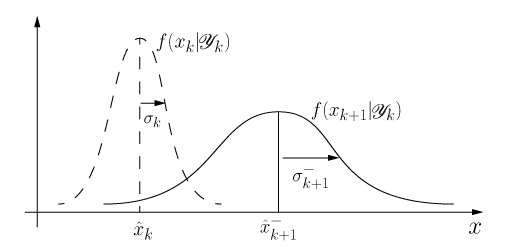
\includegraphics[width=.5\textwidth]{example_propagation.png}
	\caption{Density propagation.}
\end{figure}

You now observe your position at regular intervals $\Delta t$ with a noisy sensor that we will model as follow.
\begin{equation}\label{eq:motionobs}
y_k=x_k+v_k
\end{equation}
where $v \sim N(0,\sigma_v^2)$.
\eqref{eq:motionobs} is our \textit{observation equation}. We will asume a unique source of measurement for simplicity.
The random variables $\Delta w_k$ and $v_k$ represent respectively the model and measurement noise and are assumed to be independent of each other (both assumed to have a constant distribution for simplicity).\\
%, and with normal probability distribution:
%\begin{align*}
%w^x&\sim N(0,\sigma^x)\\
%w^y&\sim N(0,\sigma^y)\\
%\end{align*}
\\
At this point, we have two Gaussian densities containing information available for estimating your position $x_k$. One encompassing all the information before the measurement $N(\hat{x}_{k+1}^-,(\sigma_{k+1}^-)^2)$, and the other being the information provided by the measurement itself $N(x_{k+1},\sigma_v^2)$. As shown in proposition \ref{prop:UniNormal} from appendix \ref{app:UniNormal}, the combined density is Gaussian with mean
\begin{align}\label{eq:motionCorrExp}
\hat{x}_{k+1}&=\frac{(\sigma_{k+1}^-)^2}{(\sigma_{k+1}^-)^2+\sigma_v^2} \hat{x}_{k+1}^-+\frac{\sigma_v^2}{(\sigma_{k+1}^-)^2+\sigma_v^2}y_{k+1} \notag\\
&=\hat{x}_{k+1}^-+K_{k+1}(y_{k+1}-\hat{x}_{k+1}^-)
\end{align}
and variance
\begin{align}\label{eq:motionCorrVar}
\sigma_{k+1}^2&=\frac{(\sigma_{k+1}^-)^2\sigma_v^2}{(\sigma_{k+1}^-)^2+\sigma_v^2} \notag \\
&=(\sigma_{k+1}^-)^2-K_{k+1}(\sigma_{k+1}^-)^2
\end{align}
with 
$$K_{k+1}=\frac{(\sigma_{k+1}^-)^2}{(\sigma_{k+1}^-)^2+\sigma_v^2}$$ called the \textit{Kalman gain} and $(y_{k+1}-\hat{x}_{k+1}^-)$ is called the \textit{measurement innovation} or \textit{residual}. 
\\
\begin{remark}
The first term in equation \eqref{eq:motionCorrExp} is the state estimate at time $k+1$. This would be the state estimate if we didn't have a measurement. %In other words, the state estimate propagates in time just like the state vector. 
The second term is called the correction term, and it represents how much to correct the propagated estimate due to the observation.
\end{remark}

\begin{remark}
Note that, from \eqref{eq:motionCorrVar}, $\sigma_{k+1} \leq \sigma^-_{k+1}$ and $\sigma_{k+1} \leq \sigma_v$, which means that the uncertainty in the estimate of position has been reduced by combining the information $y_{k+1}$.
\end{remark}
%Note that, from ()
%\begin{equation}
%\lim_{\sigma_v^2 \to +\infty}K_{k+1}=0 \Rightarrow 
%\left\{ \begin{array}{lcrcr}
%          \hat{x}_{k+1}=\hat{x}_{k+1}^-  \\ 
%          \sigma_{k+1}^2=(\sigma_{k+1}^-)^2 \\ 
%        \end{array} \right. 
%\end{equation}
%This means that we will put little confidence in a very noisy observation and would therefore weight it lightly. Alternatively,
%\begin{equation}
												%\lim_{\sigma_w^2 \to +\infty}(\sigma_{k+1}^-)^2=\sigma_x^2 \Rightarrow 
%\lim_{\sigma_w^2 \to +\infty}K_{k+1}=1 \Rightarrow 
%\left\{ \begin{array}{lcrcr}
%          \hat{x}_{k+1}=y_{k+1}  \\ 
%          \sigma_{k+1}^2=0 \\ 
%        \end{array} \right. 
%\end{equation}
%In that case we are not certain of the ouput of the state model and therefore would weight the measurement heavily.

\begin{remark}
The state vector has two values at any given time $k$, that is the the prior value $x_k^-$ (predicted value before the update) and the posterior value $x_k$ (the corrected value after the update).
\end{remark}

The \textit{model equation} \eqref{eq:motion} along with the \textit{observation equation} \eqref{eq:motionobs} constitute the \textit{linear state space model}. The equations \eqref{eq:motionCorrExp} and \eqref{eq:motionCorrVar} characterising recursively the posterior density $N(\hat{x}_{k+1}, \sigma_{k+1}^2)$ defines the Kalman filter.
\\
\\
\begin{figure}[h!]
	\centering
	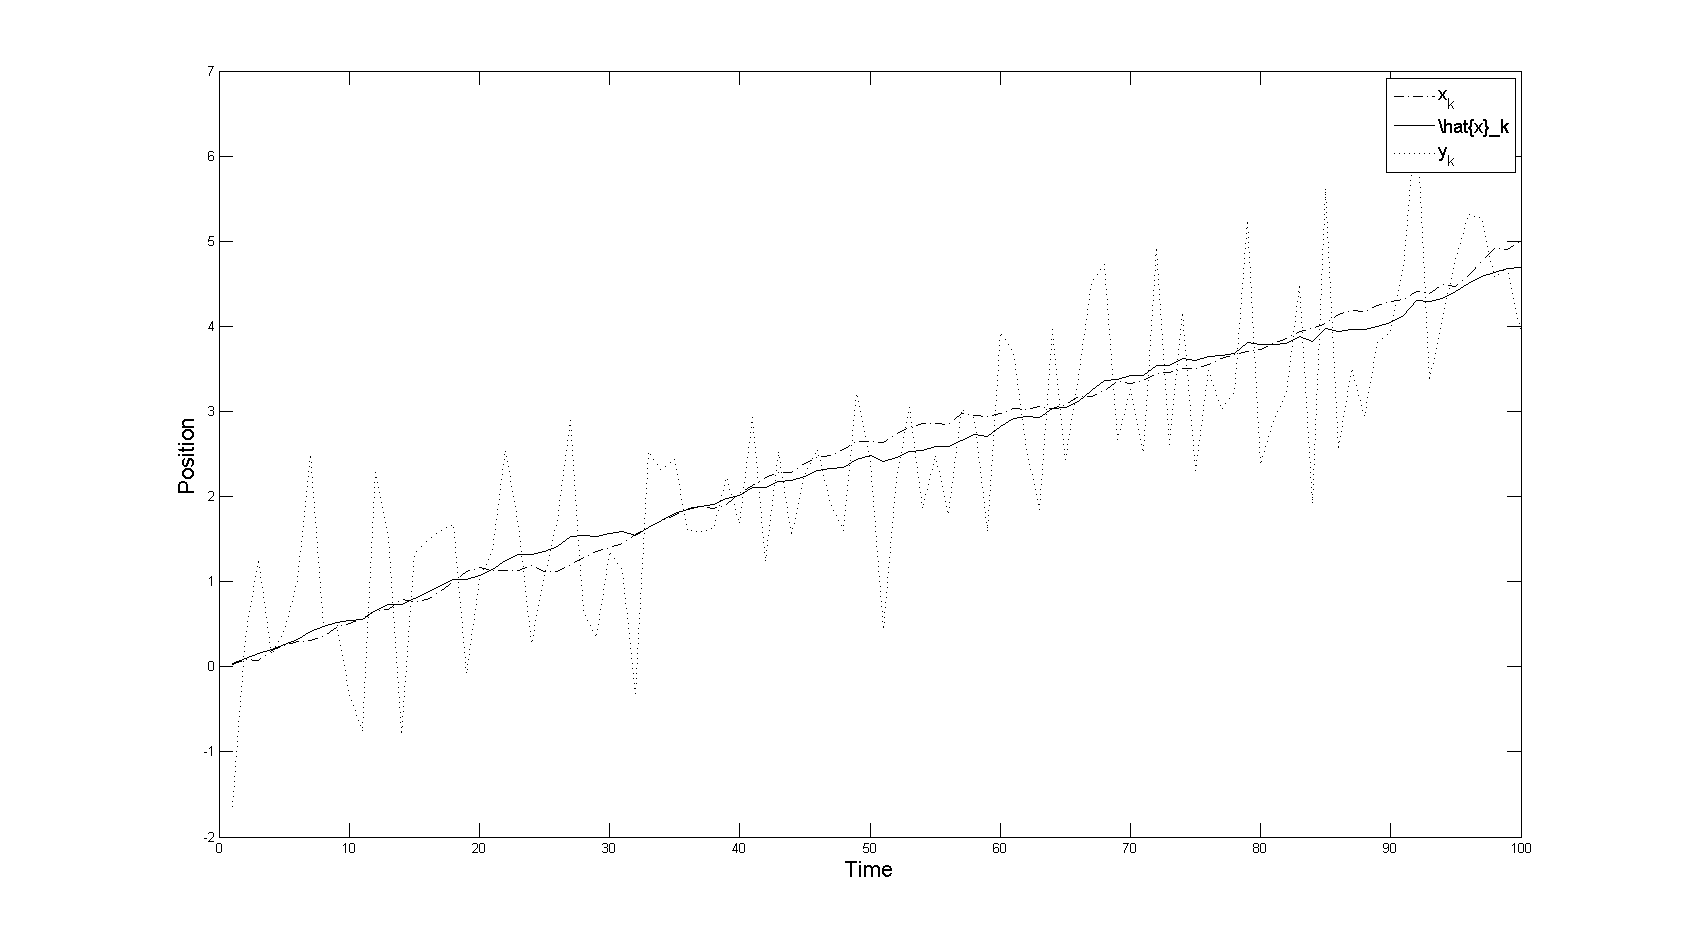
\includegraphics[width=1.1\textwidth]{example_TS.png}
	\caption{Estimated position}
	\caption*{Parameters: $T=1$, $dt=1/100$; Volatilities: $\sigma_w=0.3\%$, $\sigma_v=1$; Initial conditions: $x_0=0$, $y_0=0$}
\end{figure}

\begin{table}[h!]
  \begin{center}
    \begin{tabular}{ c  c  p{10cm} }
    \hline
		 & & Definition\\ \hline
		$x_k$ & & State (one-dimensional location).\\
		$u_k$ & & Speed.\\
		$w_k$ & & Process noise.\\
		$y_k$ & & Measurement.\\
		$v_k$ & & Measurement noise.\\
		$\hat{x}^-_k$ & $\hat{x}_{k|k}$ & Prior estimate of $x_k$, conditioned on all prior measurements except the one at time $k$.\\
		$(\sigma_{k}^-)^2$ & & Prior variance of $x_k$.\\
		$\hat{x}_k$ & $\hat{x}^+_k$ & Posterior estimate of $x_k$, conditioned on all available measurements at time $k$.\\
		$\sigma_{k}^2$ & & Posterior variance of $x_k$.\\
    \hline
    \end{tabular}
  \end{center}
  \caption{Notations.}
\end{table}






\newpage
\subsection{Matlab Algorithm}
\lstinputlisting[language=C]{../code/examples/kalmanPosition.m}




%\subsection{Matrix}
%In our case, there are different observations related to the same state variable.
%We will allow for a vector valued observation.
%\begin{equation*}
%p(y|x)=p(y_1, y_2|x)=p(y_1|x)p(y_2|x)
%\end{equation*}




\newpage
\section{Drift Estimation Simulation}
\subsection{Main Function}
\lstinputlisting[language=C]{../code/main/main.m}







\subsection{Price Simulation}
%We will be using the Euler-Maruyama method to simulate $\lambda(t)$. The remaining process will as they have no closed form solutions
The following algorithm is simulating the following processes
\begin{equation*}
%\boxed{
\left\{ \begin{array}{lcrcrcr}
			\lambda_{k+1} & = & \lambda_k &+& \kappa(\bar{\lambda}-\lambda_k)\Delta t & + & \sigma_\lambda \Delta W_k\\
          S_{k+1} & = & S_{k} & + & (r-q+\sigma\lambda_k)S_k \Delta t & + & \sigma S_k \Delta W_k \\ 
          F_{k+1} & = & F_{k} & + & \sigma\lambda_k F_k \Delta t & + & \sigma F_k \Delta  W_k \\ 
          C_{k+1} & = & C_{k} & + & (r+\sigma_c\lambda_k)C_k \Delta t & + & \sigma_c C_k \Delta  W_k 
        \end{array} \right. 
%}
\end{equation*}
and save them on file.
\lstinputlisting[language=C]{../code/main/simulate.m}





\subsection{Implied Volatility}
\lstinputlisting[language=C]{../code/main/implied_vol.m}





\subsection{Kalman Filtering Estimation}
\lstinputlisting[language=C]{../code/main/estimate.m}





\newpage
\section{References}

1. Finite Difference Methods, course notes, M. Davis.\\
\\
2. Mathematical Option pricing, course notes, C. Barnet. \\
\\
3. Estimation of Diffusion Parameters by Nonparametric Drift Function Model, Isao Shoji. \\
\\
4. Nonparametric state estimation of diffusion process, Isao Shoji.\\
\\
5. Approximating a Diffusion by a Hidden Markov Model, I. Kontoyiannis, S.P. Meyn, 2009.\\
\\
6. Bond pricing in a hidden Markov model of the short rate, Camilla Landen, 2000.\\
\\
7. Filtering Equity Risk Premia from Derivative Prices, Ramaprasad Bhar , Carl Chiarella and Wolfgang Runggaldier, 2001.\\
\\
8. On estimation of volatility for short time series of stock prices, Nikolai Dokuchaev, 2010.\\
\\
9. Recursive Bayesian Estimation: Navigation and Tracking Applications, Niclas Bergman, 1999.\\
\\
10. An Algorithmic Introduction to Numerical Simulation of Stochastic Differential Equations, Desmond J. Higham, 2001.\\
\\
11. Market microstructure theory, Maureen O'Hara, Wiley-Blackwell, 1997.\\
\\
12. Implied Volatility: Statics, Dynamics, and Probabilistic Interpretation, Roger W. Lee, 2002.\\
\\
13. Martingale methods in financial modeling, Marek Musiela and Marek Rutkowski.\\
\\
14. The calculation of implied variances from the Black-Scholes model, S. Manaster, G. Koehler, 1982.\\
\\
%(very good)
15. Bayesian Statistics for evaluation Research - An Introduction, William E. Pollard, 1986.\\
\\
16. Nonparametric Estimation of Trends in Linear Stochastic Systems, Ian W. McKeague, Tiziano Tofoni, 1989. \\%also: Statistical Inference in stochastic Process, N.U. Prabhu, I.V. Basawa, [book]
\\
17. Stochastic processes and filtering theory, Jazwinski, Andrew H., 1970.\\
\\
18. An Introduction To Nonlinear Filtering, M. H. Davis, Steven I. Marcus, .\\
\\
19. Calibration in a Bayesian modelling framework, Michiel J.W. Jansen, Thomas J. Hagenaars, 2006.\\
\\
20. Bayesian Filtering: From Kalman Filters to Particle Filters and Beyond, Zhe Chen, 2003.\\
\\
21. Maximum Likelihood Estimates Of Linear Dynamic Systems, H. E. Rauch, 1965.\\
\\
22. A Bayesian Approach to Problems in Stochastic Estimation and Control, Y.C. Ho and R.C. K. Lee, 1964.\\
\\
23. An application of the Kalman Filter: Pairs Trading (lecture notes), Ajay Jasra, 2011.\\
\\
24. Statistical Arbitrage and High-Frequency Data with Application to Eurostoxx 50 Equities, Dunis, Giorgioni, Laws, Rudy, 2010.\\
\\
25. Pairs Trading, R. J. Helliott, J. Van Der Hoek, W. P. Malcolm, 2005.\\
\\
26. Adaptive Kalman Filter for Noise Identification, M.Oussalah, J. De Schutter, 2003. \\
\\
27. Analysis of Kalman Filter with Correlated Noises under Different Dependence, L. Ma, H. Wang, J. Chen, .\\
\\
28. Optimal State Estimation,  D. Simon, 2006.\\
\\
29. Optimal Filtering, B.D.O Anderson, J.B.Moore, 1979.\\
\\
30. An Ornstein-Uhlenbeck Framework for Pairs Trading, S. Rampertshammer, 2007.\\
\\
%very good
31. Understanding the Kalman Filter, R. J. Meinhold, N. D. Singpurwall, 1983.\\
\\
32. Admissible Strategies in Semimartingale Portfolio Selection, S. Biagini, A. Cerny, 2011.\\
\\
33. Statistical Inference from Sampled Data for Stochastic Processes, B. L. S. Prakasa Rao, 1988.\\
\\
34. Stochastic models, estimation, and control, Volume 1, Peter S. Maybeck, 1979.
\end{document}




Recall that 
\begin{equation}
N(x)=P(X \leq x)=\int_{- \infty}^{x}\phi(u)du=\int_{- \infty}^{x}\frac{1}{\sqrt{2\pi}}e^{-\frac{u^2}{2}}du.
\end{equation}

\begin{equation}
\frac{d N(x)}{d x}=\frac{1}{\sqrt{2\pi}}e^{-\frac{x^2}{2}}.
\end{equation}

Now $X=\mu+\sigma Z$% \Rightarrow Z=\frac{X-\mu}{\sigma}$

\begin{align*}
N(x)&=P(X \leq \mu+\sigma Z)=P(Z \leq \frac{x-\mu}{\sigma})\\
&=\int_{- \infty}^{\frac{x-\mu}{\sigma}}\phi(u)du=\int_{- \infty}^{\frac{x-\mu}{\sigma}}\frac{1}{\sqrt{2\pi}}e^{-\frac{u^2}{2}}du\\
&=N(z).
\end{align*}

%\begin{equation}
%N(z)=P(Z \leq \frac{x-\mu}{\sigma})=\int_{- \infty}^{\frac{x-\mu}{\sigma}}\phi(u)du=\int_{- \infty}^{\frac{x-\mu}{\sigma}}\frac{1}{\sqrt{2\pi}}e^{-\frac{u^2}{2}}du.
%\end{equation}

\begin{align*}
\frac{d N(x)}{d x}=&\frac{d}{dx}N(z)\\
&=\frac{d z}{d x}\frac{d N(z)}{d z}\\
&=\frac{1}{\sigma}\phi(z)\\
&=\frac{1}{\sigma\sqrt{2\pi}}e^{-\frac{1}{2}\left( \frac{x-\mu}{\sigma}\right)^2}.
\end{align*}
